% !BIB TS-program = biber

\RequirePackage[l2tabu,orthodox]{nag}

% TODO: decide if one-sided/two-sided
%\documentclass[headsepline,footsepline,footinclude=false,fontsize=11pt,paper=a4,listof=totoc,bibliography=totoc,BCOR=12mm,DIV=12]{scrbook} % two-sided
\documentclass[headsepline,footsepline,footinclude=false,oneside,fontsize=11pt,paper=a4,listof=totoc,bibliography=totoc]{scrbook} % one-sided

% TODO: change citation style in settings
\PassOptionsToPackage{table,svgnames,dvipsnames}{xcolor}

\usepackage[utf8]{inputenc}
\usepackage[T1]{fontenc}
\usepackage[sc]{mathpazo}
\usepackage[ngerman,american]{babel}
\usepackage[autostyle]{csquotes}
\usepackage[%
  backend=biber,
  url=false,
  style=alphabetic,
  maxnames=4,
  minnames=3,
  maxbibnames=99,
  giveninits,
  uniquename=init]{biblatex} % TODO: adapt citation style
\usepackage{graphicx}
\usepackage{scrhack} % necessary for listings package
\usepackage{listings}
\usepackage{lstautogobble}
\usepackage{tikz}
\usepackage{pgfplots}
\usepackage{pgfplotstable}
\usepackage{booktabs}
\usepackage[final]{microtype}
\usepackage{caption}
\usepackage[printonlyused]{acronym}
\usepackage[hidelinks]{hyperref} % hidelinks removes colored boxes around references and links
\AtBeginDocument{%
	\hypersetup{
		pdftitle=\getTitle,
		pdfauthor=\getAuthor,
	}
}
\usepackage{ifthen}

\addto\extrasamerican{
	\def\lstnumberautorefname{Line}
	\def\chapterautorefname{Chapter}
	\def\sectionautorefname{Section}
	\def\subsectionautorefname{Subsection}
	\def\subsubsectionautorefname{Subsubsection}
}

\addto\extrasngerman{
	\def\lstnumberautorefname{Zeile}
}

% Themes
\ifthenelse{\equal{\detokenize{dark}}{\jobname}}{%
  % Dark theme
  \newcommand{\bg}{black} % background
  \newcommand{\fg}{white} % foreground
  \usepackage[pagecolor=\bg]{pagecolor}
  \color{\fg}
}{%
  % Light theme
  \newcommand{\bg}{white} % background
  \newcommand{\fg}{black} % foreground
}

\bibliography{bibliography}

\setkomafont{disposition}{\normalfont\bfseries} % use serif font for headings
\linespread{1.05} % adjust line spread for mathpazo font

% Add table of contents to PDF bookmarks
\BeforeTOCHead[toc]{{\cleardoublepage\pdfbookmark[0]{\contentsname}{toc}}}

% Define TUM corporate design colors
% Taken from http://portal.mytum.de/corporatedesign/index_print/vorlagen/index_farben
\definecolor{TUMBlue}{HTML}{0065BD}
\definecolor{TUMSecondaryBlue}{HTML}{005293}
\definecolor{TUMSecondaryBlue2}{HTML}{003359}
\definecolor{TUMBlack}{HTML}{000000}
\definecolor{TUMWhite}{HTML}{FFFFFF}
\definecolor{TUMDarkGray}{HTML}{333333}
\definecolor{TUMGray}{HTML}{808080}
\definecolor{TUMLightGray}{HTML}{CCCCC6}
\definecolor{TUMAccentGray}{HTML}{DAD7CB}
\definecolor{TUMAccentOrange}{HTML}{E37222}
\definecolor{TUMAccentGreen}{HTML}{A2AD00}
\definecolor{TUMAccentLightBlue}{HTML}{98C6EA}
\definecolor{TUMAccentBlue}{HTML}{64A0C8}

% Settings for pgfplots
\pgfplotsset{compat=newest}
\pgfplotsset{
  % For available color names, see http://www.latextemplates.com/svgnames-colors
  cycle list={TUMBlue\\TUMAccentOrange\\TUMAccentGreen\\TUMSecondaryBlue2\\TUMDarkGray\\},
}

% Settings for lstlistings
\lstset{%
  basicstyle=\ttfamily,
  columns=fullflexible,
  autogobble,
  keywordstyle=\bfseries\color{TUMBlue},
  stringstyle=\color{TUMAccentGreen},
  captionpos=b
}


% TODO: change thesis information
\newcommand*{\getUniversity}{Technische Universität München}
\newcommand*{\getFaculty}{Informatics}
\newcommand*{\getDegree}{Informatics}
\newcommand*{\getSchool}{Computation, Information and Technology}
\newcommand*{\getTitle}{An Approach to Coreference Resolution and Formula Grounding for Mathematical Identifiers using Large Language Models}
\newcommand*{\getTitleGer}{Ein Ansatz zur Auflösung von Koreferenzen und zur Ermittlung von Formeln für mathematische Symbole mit Hilfe von Large Language Models}
\newcommand*{\getAuthor}{Aamin Dev}
\newcommand*{\getDoctype}{Bachelor's Thesis}
\newcommand*{\getSupervisor}{Prof. Dr. Georg Groh, Prof. Dr. Yusuke Miyao}
\newcommand*{\getAdvisor}{Miriam Anschütz, Takuto Asakura}
\newcommand*{\getSubmissionDate}{2023-09-15}
\newcommand*{\getSubmissionLocation}{Garching bei. München}

\begin{document}

% Set page numbering to avoid "destination with the same identifier has been already used" warning for cover page.
% (see https://en.wikibooks.org/wiki/LaTeX/Hyperlinks#Problems_with_Links_and_Pages).
\pagenumbering{alph}
\begin{titlepage}
  % HACK for two-sided documents: ignore binding correction for cover page.
  % Adapted from Markus Kohm's KOMA-Script titlepage=firstiscover handling.
  % See http://mirrors.ctan.org/macros/latex/contrib/koma-script/scrkernel-title.dtx,
  % \maketitle macro.
  \oddsidemargin=\evensidemargin\relax
  \textwidth=\dimexpr\paperwidth-2\evensidemargin-2in\relax
  \hsize=\textwidth\relax

  \centering

  \IfFileExists{logos/tum-\fg.pdf}{%
    \includegraphics[height=20mm]{logos/tum-\fg.pdf}
  }{%
    \vspace*{20mm}
  }

  \vspace{5mm}
  {\huge\MakeUppercase{School of \getSchool{} --- \getFaculty{}} \par}

  \vspace{5mm}
  {\large\MakeUppercase{\getUniversity{}} \par}

  \vspace{15mm}
  {\Large \getDoctype{} in \getDegree{} \par}

  \vspace{10mm}
  {\huge\bfseries \getTitle{} \par}

  \vspace{10mm}
  {\LARGE \getAuthor{}}

  \IfFileExists{logos/faculty-\fg.pdf}{%
    \vfill{}
    \includegraphics[height=20mm]{logos/faculty-\fg.pdf}
  }{}
\end{titlepage}


\frontmatter{}

\begin{titlepage}
  \centering

  \IfFileExists{logos/tum.png}{%
    
\includegraphics[height=20mm]{logos/tum.png}
  }{%
    \vspace*{5mm}
  }

  \vspace{5mm}
  {\huge\MakeUppercase{School of \getSchool{} --- \getFaculty{}} \par}

  \vspace{5mm}
  {\large\MakeUppercase{\getUniversity{}} \par}

  \vspace{15mm}
  {\Large \getDoctype{} in \getDegree{} \par}

  \vspace{10mm}
  {\huge\bfseries \getTitle{} \par}

  \vspace{10mm}
  {\huge\bfseries \foreignlanguage{ngerman}{\getTitleGer{}} \par}

  \vspace{5mm}
  \begin{tabular}{l l}
    Author:          & \getAuthor{}         \\
    Supervisor:      & \getSupervisor{}     \\
    Advisor:         & \getAdvisor{}        \\
    Submission Date: & \getSubmissionDate{} \\
  \end{tabular}

  \IfFileExists{logos/faculty-\fg.pdf}{%
    \vfill{}
    \includegraphics[height=20mm]{logos/faculty-\fg.pdf}
  }{}
\end{titlepage}

\thispagestyle{empty}
\vspace*{0.8\textheight}
\noindent
I confirm that this \MakeLowercase{\getDoctype{}} is my own work and I have documented all sources and material used.

\vspace{15mm}
\noindent
\getSubmissionLocation{}, \getSubmissionDate{} \hspace{50mm} \getAuthor{}

\cleardoublepage{}

\addcontentsline{toc}{chapter}{Acknowledgments}
\thispagestyle{empty}

\vspace*{20mm}

\begin{center}
    {\usekomafont{sectioning}\usekomafont{section} Acknowledgments}
\end{center}

\vspace{10mm}

%TODO: Acknowledge
TODO: Acknowledge supervisors, advisors, family, friends.

\cleardoublepage{}

\chapter{\abstractname}

%TODO: Abstract

\microtypesetup{protrusion=false}
\tableofcontents{}
\microtypesetup{protrusion=true}

\mainmatter{}

% !TeX root = ../main.tex
% Add the above to each chapter to make compiling the PDF easier in some editors.

\chapter{Introduction}\label{chapter:introduction}

\section{Section}
Citation test~\parencite{asakura2020towards}.

\chapter{Related Work}\label{chapter:related_work}

Mathematical Language Processing (MLP) is a burgeoning area of research, focusing on the complexities of understanding, annotating, and disambiguating mathematical text. This chapter critically reviews seminal papers that have significantly influenced this domain, contextualising our current study.

\section{Understanding Mathematical Text and Formulae}

The early work by \citet{grigore2009towards} is a foundational study in mathematical language processing. Grigore emphasised the importance of linguistic context in deciphering mathematical formulae, primarily focusing on symbolic expressions within mathematical narratives. While this work laid the groundwork, it did not delve into automation or using machine-learning models for annotation.

Building upon this, the MLP project by \citet{pagael2014mathematical} introduced a novel approach employing \ac{POS} tag-based distances to estimate the probabilities of identifier-definition relationships. This approach contrasts with traditional pattern-matching techniques, offering a more nuanced understanding of mathematical identifiers. However, it still relies on manual intervention for accurate results.

Most recently, \citet{meadows2022survey} extended the discourse by advocating using transformer models like GPT for formula retrieval. Meadows emphasised the role of informal mathematical text in quantitative reasoning, opening the door for more automated approaches. Unlike our study, Meadows' research focuses not on annotation automation but on formula retrieval.

\section{Foundational Frameworks and Automation}

The pioneering work by \citet{asakura2020towards} is a cornerstone. Asakura and colleagues introduced MioGatto, a cutting-edge annotation tool that anchors or grounds mathematical formulae. Their work highlights the importance of MLP in deciphering STEM manuscripts, but it does not explore the automation of the annotation process, which is the focal point of our study.

\citet{ding2022gpt} and \citet{schubotz2017evaluating} collectively highlight the potential of automation in data annotation. Ding specifically focuses on the role of GPT-3 in reducing annotation overheads but does not delve into the evaluation metrics or the semantic accuracy of the annotations. Schubotz, on the other hand, sets the stage for automated extraction frameworks for mathematical identifier definitions but does not employ \ac{LLMs} for this purpose.

\citet{alexeeva2020mathalign} extend this discourse by introducing machine reading techniques for extracting mathematical concepts. Their rule-based strategy aligns \LaTeX \space representations with textual counterparts, offering a more structured but less flexible approach than our data-driven methodology.

\section{The Role of Large Language Models (LLMs) and Pre-trained Frameworks}

The advent of pre-trained models like "MathBERT" \citep{peng2021mathbert} and the evaluation of GPT-3.5 \citep{he2023annollm} mark significant milestones. MathBERT is fine-tuned for decoding mathematical formulae and emphasises the importance of context. However, it is not designed for annotating mathematical identifiers, which is the primary focus of our study.

The research on GPT-3.5 evaluates its efficacy as a robust annotator and questions its potential to replace traditional crowdsourced methods. While this work aligns closely with our study, it does not provide a comprehensive evaluation using metrics like CoNLL or semantic accuracy, which are central to our research.

\section{Summary}

The body of work reviewed here offers a comprehensive landscape of the challenges and innovations in MLP. These cornerstone studies provide invaluable insights and reveal gaps our research aims to fill. As the field evolves, our study builds upon these foundational works, introducing automation and comprehensive evaluation metrics to advance the domain of mathematical identifier annotation.

\chapter{Methodology}\label{chapter:methods}

This chapter describes the methodology employed in this research, encompassing three core stages: 1) pre-processing of mathematical identifiers, 2) dictionary construction, and 3) association of individual IDs to description (annotation) instances. The process uses \LaTeX ML utilities and explores the capabilities of \ac{LLMs} to automate the annotation of mathematical identifiers. Here, we present the transitions from source materials to machine-readable formats and from dictionary formulation to final annotation. The entire code is available at \url{https://github.com/babyygemperor/grounding-of-formulae}.

Before delving into the specifics, it is crucial to understand the structure of \\ MioGatto\footnote{\url{https://github.com/wtsnjp/MioGatto/}} \citep{asakura2021miogatto}, the tool we aim to automate. MioGatto contains three core files: 
\begin{enumerate}
    \item \texttt{source.html}—a pre-processed HTML file suitable for web rendering of the given paper, illustrated in Figure \ref{fig:miogatto-sources}
    \item \texttt{mcdict.json}—a JSON file containing a list of dictionary of possible descriptions for each identifier (Figure \ref{fig:miogatto-data}a), 
    \item \texttt{anno.json}—another JSON file that holds each identifier's index of the chosen description (Figure \ref{fig:miogatto-data}b).
\end{enumerate}

The generation of these three files corresponds to the three first sections in this chapter. 
Section \ref{sec:pre-processing} focuses on creating \texttt{source.html}. 
Section \ref{sec:dic-generation} covers the generation of \texttt{mcdict.json}, and Section \ref{sec:annotation} addresses \texttt{anno.json}. The three core files are interlinked by IDs generated during pre-processing. The structure of the JSON files is depicted in Figure \ref{fig:miogatto-data}.

%% Maybe this figure should also show the "web rendering" described above for increased readability.
\begin{figure}[htpb]
  \centering
    \begin{minipage}{1\textwidth}
      \lstinputlisting[language=html]{sources/source.html}
    \end{minipage}
  \caption[LaTeXML Pre-processing]{HTML format of "A Logic of Expertise" \citep{singleton2021logic} obtained after transforming the \LaTeX \space source using \LaTeX ML. This machine-readable format serves as the basis for dictionary generation and annotation in MioGatto.}\label{fig:miogatto-sources}
\end{figure}

\begin{figure}[htpb]
  \centering
  \subfloat[mcdict.json]{
    \begin{minipage}{1\textwidth}
      \lstinputlisting[language=python]{sources/mcdict.json}
    \end{minipage}
  }
  \quad 
  \subfloat[anno.json]{
    \begin{minipage}{1\textwidth}
      \lstinputlisting[language=python]{sources/anno.json}
    \end{minipage}
  }
  \caption[LaTeXML Preprocessing]{JSON file structure in MioGatto. The dictionary file contains a list of mathematical identifiers (keys) and their possible descriptions (values). The annotation file holds the index of the chosen description for each identifier.}\label{fig:miogatto-data}
\end{figure}

\section{Pre-processing}\label{sec:pre-processing}

Initially, we considered parsing the \LaTeX \space code directly via GPT-based LLMs, owing to their frequent training on \LaTeX \space documents. \LaTeX \space has a more decent semantic layer to mathematical identifiers than ASCII Math and offers efficiency in token usage (see Definition~\ref{def:token}) and complexity compared to MathML. To illustrate the effectiveness of different encodings, Table \ref{fig:ascii-math} displays various representations of identical formulae, comparing \LaTeX, ASCII Math, and MathML (XML) regarding readability and token count.


\begin{figure}[htpb]
  \centering
  \begin{lstlisting}[language=python]
{    
    "$\\equiv$": "Logical equivalence operator",
    "$\\phi$": "A formula in the language $\\cL$",
    "$\\cL$": "Language of expertise and soundness",
    "$\\prop$": "Countable set of propositional variables",
    "$\\univ$": "Universal modality",
    "$\\orr$": "Disjunction operator",
    "$\\subseteq$": "Subset or equal to",
    "$\\in$": "Element of a set",
    "$\\cap$": "Intersection of two sets",
    "$\\subseteq$": "Subset or equal to",
    "$\\emptyset$": "Empty set",
    "$\\sat$": "Satisfaction relation",
    "$\\neg$": "Negation operator",
    "$\\and$": "Conjunction operator",
    "$\\|\phi\\|_M$": "Set of states where $\\phi$ is true in model $M$",
    "$\\forall$": "Universal quantifier"
}
  \end{lstlisting}
  \caption[GPT Dictionary from LaTeX]{Dictionary generated by GPT-3.5 using \LaTeX \space as the source demonstrating LLMs ability to generate a comprehensive and well-structured dictionary of mathematical identifiers and their descriptions.}\label{fig:latex-dict}
\end{figure}

While \LaTeX \space yielded a high-quality dictionary in our initial experiments, a challenge emerged in mapping the keys of the generated \LaTeX \space dictionary to their rendered instances in the final annotation. This necessitated an array of complex heuristics to convert the dictionary generated using \LaTeX \space as source (Figure \ref{fig:latex-dict}) to a MioGatto dictionary (Figure \ref{fig:miogatto-data}a). Converting complex \LaTeX \space equations to ASCII Math would have alleviated the heuristics issue, but it was deemed infeasible due to ASCII Math's limitations of expressing rich content. This also led us to rule out directly ingesting XML because of the prohibitive token count and because \ac{LLMs} lacked training on XML, leading them to generate nonsensical outputs. Consequently, we opted for a pre-processing step to retrieve the identifiers in a format that removed the need for intricate heuristics.


\LaTeX ML\footnote{\url{https://math.nist.gov/~BMiller/LaTeXML/}} \citep{ginev2011latexml} served as the tool of choice for this pre-processing step. The rationale behind this conversion is clear: HTML stands as the source view for further processing with MioGatto and formula grounding. Quite conveniently, \LaTeX ML automatically identifies mathematical symbols and embeds them in an \lstinline{<mi>} tag, making the output machine-readable. We subsequently transform the HTML into our variant of ASCII Math with the following command.

\begin{lstlisting}[language=bash]
latexmlc --preload=[nobibtex,ids,mathlexemes,localrawstyles]latexml.sty
     --format=html5 --pmml --cmml --mathtex --nodefaultresources 
     --dest=<output HTML file> <input TeX file>
\end{lstlisting}

While this format conveys less information than \LaTeX, the robust capabilities of LLMs compensate for this limitation, yielding comparable results. After the HTML generation, MioGatto's pre-processing tool runs to create a template for the dictionary and annotations with the following command: 
  \begin{lstlisting}[language=bash]
    python -m tools.preprocess <HTML file>
  \end{lstlisting}



\begin{table}[htpb]
  \centering
  \subfloat[Quadratic Equation]{%
    \begin{tabular}{llr}
      \hline
      Encoding & Formula & Tokens\\
      \hline
      \LaTeX & \( x = \frac{-b \pm \sqrt{b^2 - 4ac}}{2a} \) & 24 \\
      ASCII Math & \texttt{x = (-b +/- sqrt\{b\^{}2 - 4ac\})/(2a)} & 23 \\
      XML & Shown in Appendix \ref{app:xml_quadratic} & 387 \\
      \hline
    \end{tabular}
  }
  \quad 
  \subfloat[Ampere's Circuit Law]{%
    \begin{tabular}{llr}
      \hline
      Encoding & \begin{tabular}[t]{@{}l@{}}Formula\end{tabular} & Tokens\\
      \hline
      \LaTeX & \( \oint_C \vec{B}\circ \mathrm{d}\vec{l} = \mu_0 \left( I_{\text{enc}} + \varepsilon_0 \frac{\mathrm{d}}{\mathrm{d} t} \int_S \vec{E} \circ \hat{n}\; \mathrm{d} a \right) \) & 84 \\
      ASCII Math & \begin{tabular}[t]{@{}l@{}}\texttt{oint\_C (B . dl)=mu\_0*(I\_\{enc\} +} \\ \texttt{eps\_0 * d/dt * int\_S (E . n\_\{hat\}) da)}\end{tabular} & 42 \\
      XML & Shown in Appendix \ref{app:xml_ampere} & 929 \\
      \hline
    \end{tabular}
  }
  \caption[Token Usages]{Token usages of three different types of encoding (\LaTeX, ASCII Math, and XML).}
  \label{fig:ascii-math}
\end{table}



\section{Dictionary Generation}\label{sec:dic-generation}

Transforming raw HTML data into a comprehensive dictionary required several different tactics. Initial attempts included \ac{POS} tagging. It seemed convenient as, in most academic texts, identifier definitions are placed either before or after the identifier's first introduction.

For instance, within the excerpt from the paper "A Logic of Expertise" by  \citet{singleton2021logic} as shown in Figure \ref{fig:POS_right}, "$\mathsf{Prop}$" is introduced and immediately followed by its definition "\textit{A countable set of propositional variables}".

\begin{figure}[htpb]
  \centering
  \begin{tabular}{c}
  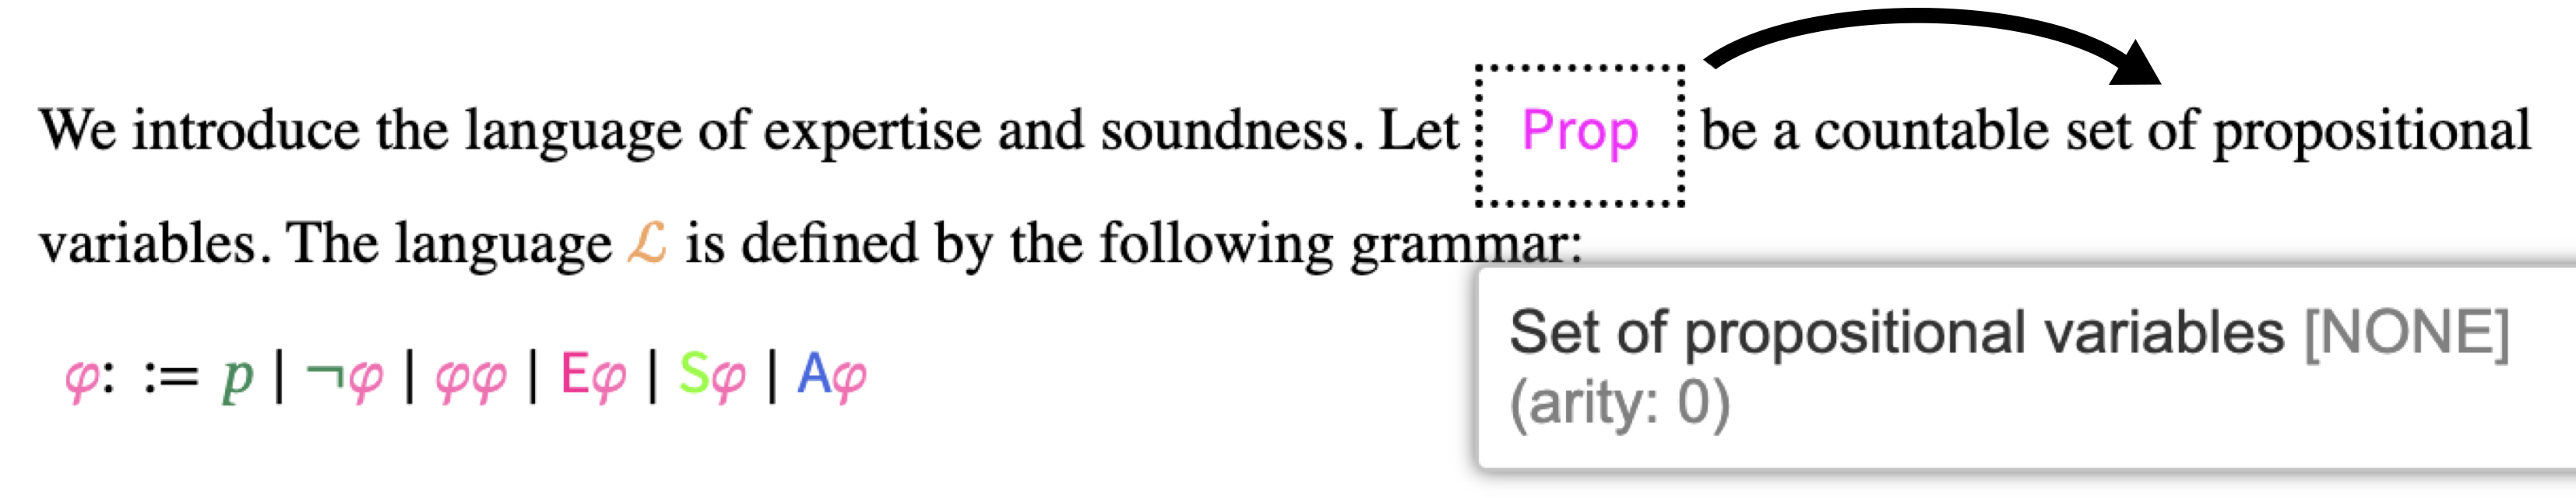
\includegraphics[width=14cm]{images/POS_right.png}
  \end{tabular}
  \caption[POS Tagging Right]{Screenshot of MioGatto showing the paper "A Logic of Expertise" with description to the right of the identifier Prop.}\label{fig:POS_right}
\end{figure}

Similarly in Figure \ref{fig:POS_left}, `$\mathcal{L}$` is described as "$language$" immediately prior to its mention.

\begin{figure}[htpb]
  \centering
  \begin{tabular}{c}
  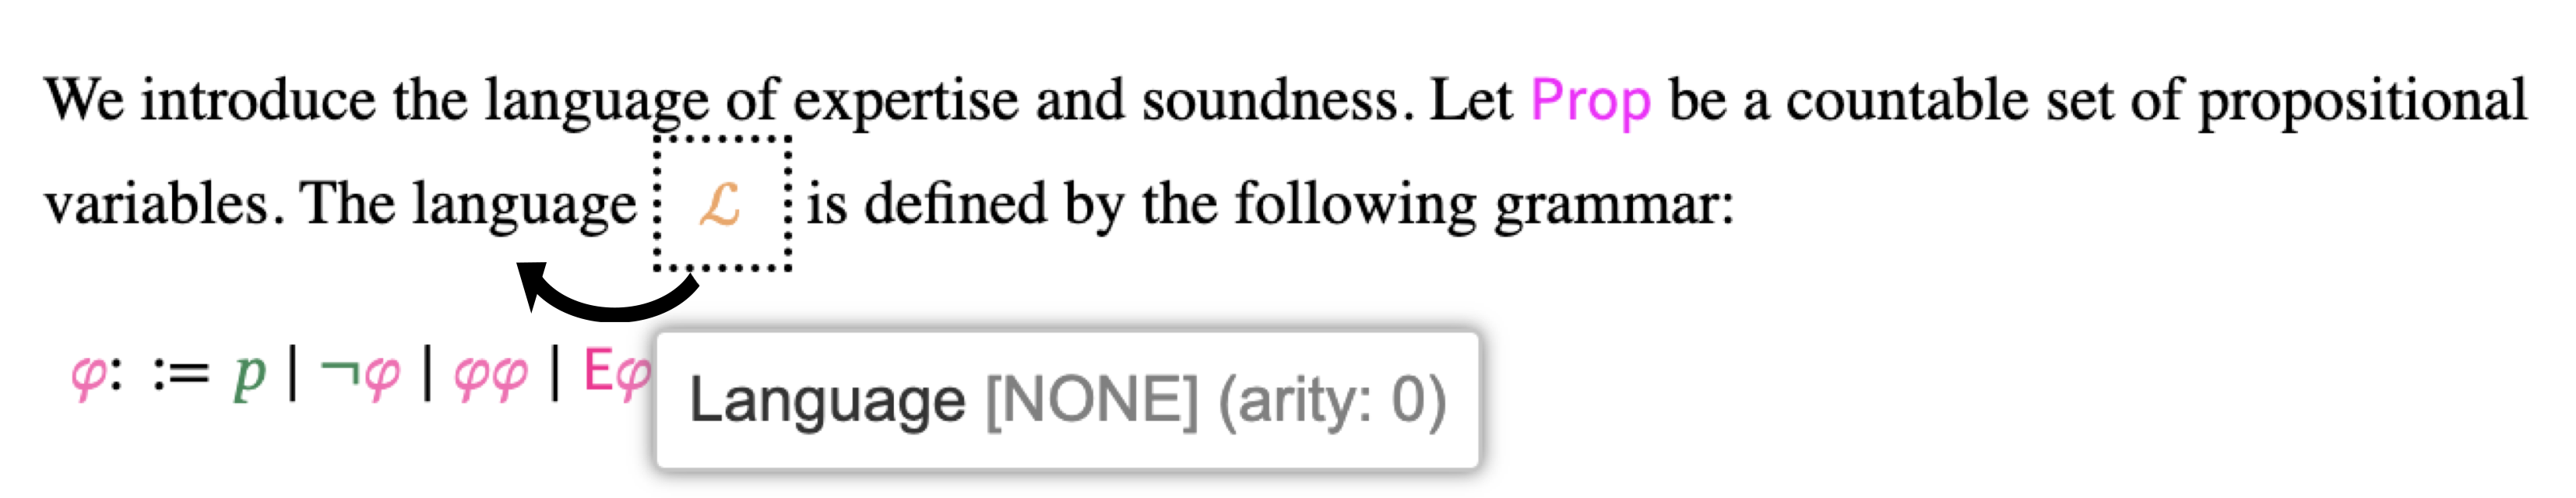
\includegraphics[width=14cm]{images/POS_left.png}
  \end{tabular}
  \caption[POS Tagging Left]{Screenshot of MioGatto showing the paper "A Logic of Expertise" with description to the left of the identifier L.}\label{fig:POS_left}
\end{figure}

While seemingly effective for cases like these, this pattern only works for some cases. In several instances across academic works, the definition does not directly proceed or follow the identifier, making POS tagging less fruitful. Take, for example, the snippet shown in Figure~\ref{fig:POS_failed} from the same paper mentioned earlier. Here, our mathematical understanding identifies "$X$" as a set, which is not readily inferred by POS tagging or formal grammar alone.

\begin{figure}[htpb]
  \centering
  \begin{tabular}{c}
  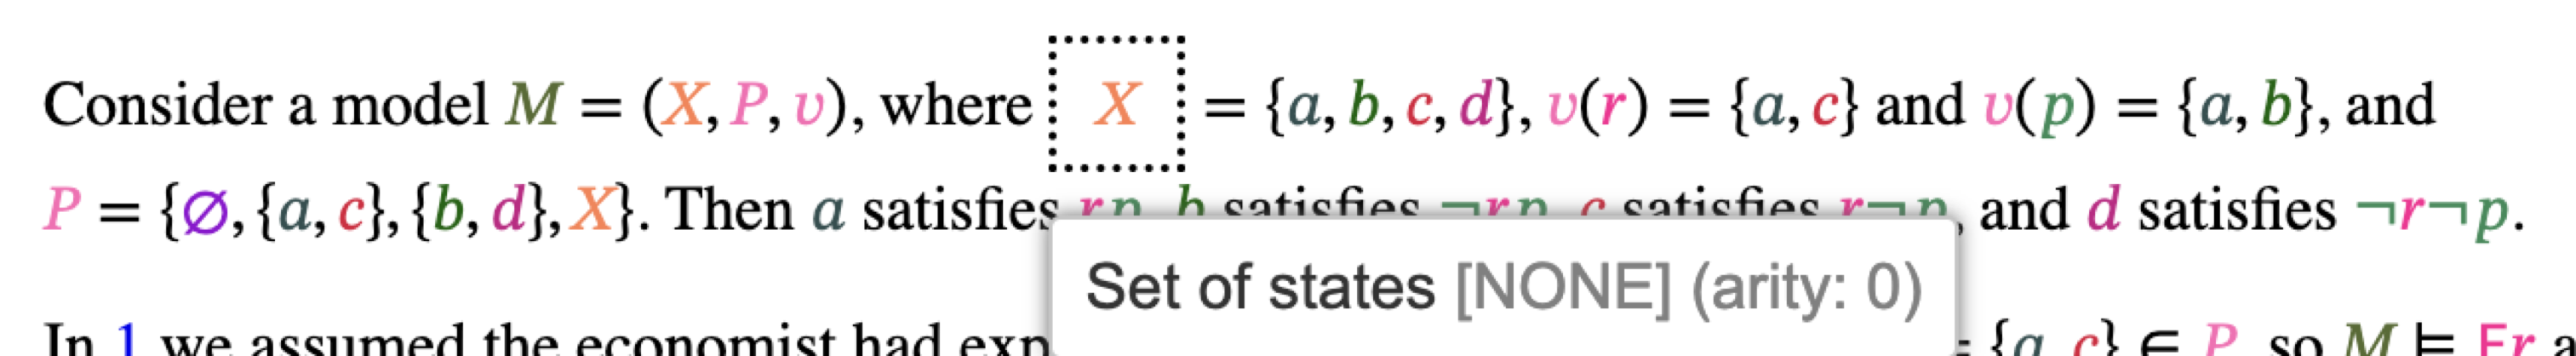
\includegraphics[width=14cm]{images/POS_failed.png}
  \end{tabular}
  \caption[POS Tagging Left]{Screenshot of MioGatto showing the paper "A Logic of Expertise" without a possible POS Tagging.}\label{fig:POS_failed}
\end{figure}

\begin{figure}[htpb]
  \centering
  \begin{tabular}{c}
  \begin{lstlisting}[language=python]
    {
        "P": [
            "Expertise set"
            "Set of properties P1, P2, P3",
            "Mapping to RP"
            "Set of all unions of equivalence classes"
        ],
        "M": [
            "Expertise model",
            "Model"
            "S5 model",
            "Non-augmented model obtained from N' by dropping the RA'
             component"
        ], 
        "p": "Proposition",
        "r": [
            "Economic recovery proposition",
            "Report proposition"
        ],
        "s", "Source"
        "L": "Language of expertise and soundness"
    }
  \end{lstlisting}
  \end{tabular}
  \caption[Response from Main Prompt for Dictionary Generation]{Response JSON from GPT using the prompt for dictionary generation containing the keys as the mathematical identifiers and the values as their possible respective definitions.}\label{fig:dic_response}
\end{figure}

This complexity led to exploring the capabilities of \ac{LLMs} like GPT-3.5 from OpenAI. While LLMs were generally designed as chat models and not specifically for mathematical text or dictionary generation, preliminary trials proved promising. Upon feeding a paragraph of text to the model through OpenAI's API, it returned a well-formatted dictionary (Figure \ref{fig:dic_response}) that was highly usable for annotation. However, an obstacle emerged that the model's context window is limited. Most of the papers we tested were (at least) 20-40 thousand tokens long, and the context window of the LLMs is not big enough to accommodate this (see Table~\ref{tab:token_counts}).
%% Better text? "20-40 thousand tokens" or "20k-40k tokens"
%% Rune: Define Tokens as roughly equivalent to the Number of Words. 

\begin{table}[h]
    \centering
    \begin{tabular}{lrr}
        \hline
        Model & Context Window (Tokens) & Chunks Size (Tokens)\\
        \hline
        GPT-3.5-turbo & 4096 & 1750 \\
        GPT-3.5-16k-turbo & 16384 & 2000 \\
        GPT-4 & 8192 & 4000 \\
        \hline
    \end{tabular}
    \caption{Token counts for different models}
    \label{tab:token_counts}
\end{table}

To deal with the overflow issue, each paper was divided into smaller chunks, approximately half the size of the respective model's context window. The context window varies for different \ac{NLP} models as well, and the chosen sizes of chunks are shown in Table \ref{tab:token_counts}. This adjustment accounted for the tokens generated by the API and made allowances for the length of our prompts. The token count was carefully reduced for GPT-3.5-16k-turbo because the model tended to generalise the description of the identifiers when there were many occurrences in larger chunk sizes.

After dividing the paper into smaller overlapping chunks, they are used as inputs to the OpenAI API iteratively to generate a dictionary associated explicitly with each chunk. The chunks were carefully constructed so they did not fragment paragraphs and thus maintained the integrity of any crucial contextual information. Furthermore, to mitigate context loss when transitioning from one chunk to another, the generated dictionary was looped back into the prompt, which ensured the LLM maintained awareness of the other possible definitions of the identifiers. The system prompt (see Definition~\ref{def:prompt}) (Figure~\ref{fig:prompt_dic_system}) was meticulously designed, through experimentation, to provide the best possible results. After the system prompt, an example of the desired dictionary format was presented, as shown in Figure \ref{fig:prompt_dic_example}. Considering this approach involves neither zero-shot learning nor one-shot/few-shot learning, we call it  'half-shot learning'. 

\begin{figure}[htpb]
  \centering
  \begin{tabular}{c}
  \begin{lstlisting}[language=python]
    {'role': 'system',
    'content': 'You are a helpful research assistant tasked with converting
    long paragraphs into a Python dictionary. The goal is to identify and 
    classify each individual mathematical symbol, variable, and identifier 
    in the text marked between "<||>". The dictionary should store the 
    identifiers as keys and their corresponding definitions as values 
    in an array format. '}
  \end{lstlisting}
  \end{tabular}
  \caption[System Prompt for Dictionary Generation]{System prompt for dictionary generation instructing the LLM to convert long paragraphs into a Python dictionary, emphasising the need to identify and classify each mathematical identifier.}\label{fig:prompt_dic_system}
\end{figure}

\begin{figure}[htpb]
  \centering
  \begin{tabular}{c}
  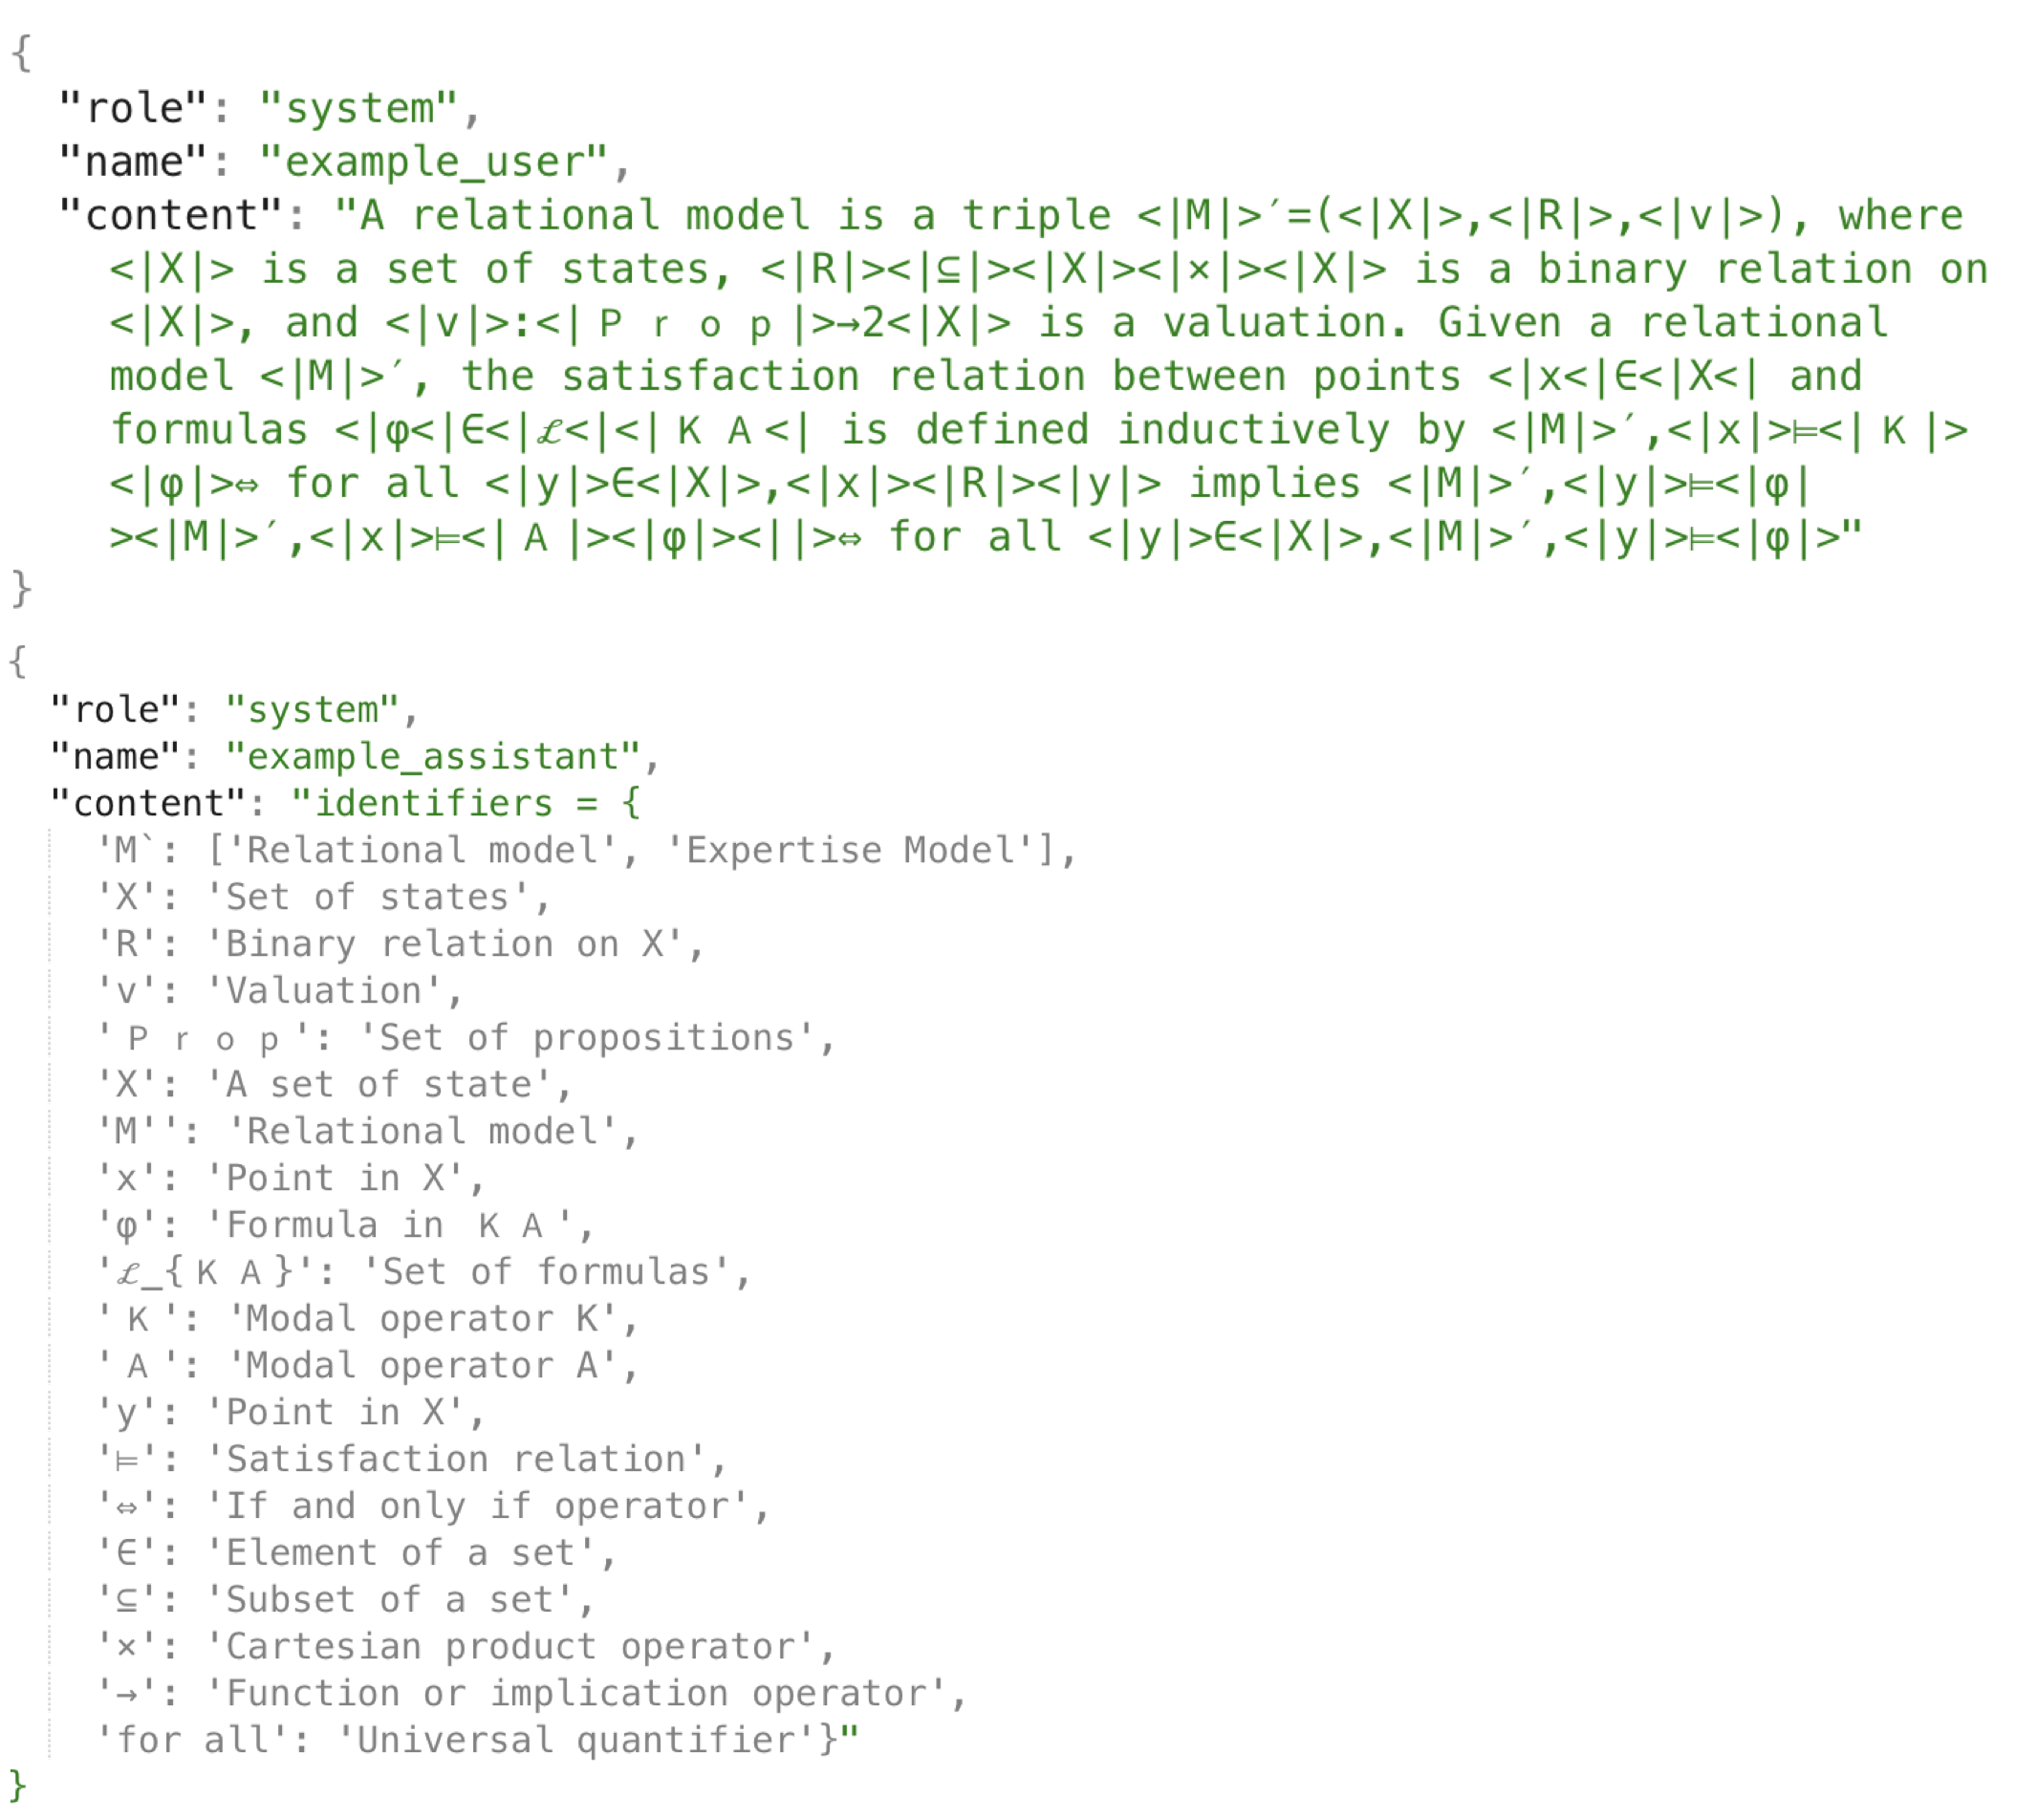
\includegraphics[width=14cm]{images/Prompt_dict_example.png}
  \end{tabular}
  \caption{An example of the desired dictionary format provided in the prompt for dictionary generation guiding the LLM to produce a dictionary with mathematical identifiers as keys and their possible descriptions as values serving as a template for the LLM, facilitating the generation of a MioGatto-compatible dictionary.}\label{fig:prompt_dic_example}
\end{figure}

The prompt containing the chunks (Figure~\ref{fig:prompt_dic}) is then forwarded to the next stage. The previously generated dictionary is attached as supplementary context to help deal with the token limit context window.
% context - contend - content is somewhat confusing.
However, if the prompt is excessively long, the previous dictionary is omitted, and this scenario is the only occurrence of context loss from one iteration to another. The chunk is submitted, and the response received is parsed and incorporated into the master dictionary. This procedure is repetitively enacted until all the chunks have passed through the LLM and a comprehensive master dictionary is generated. This essential JSON dictionary (Figure \ref{fig:dic_response}) then gets converted into a MioGatto-compatible dictionary (Figure \ref{fig:miogatto-data}a) using basic mapping techniques.

\begin{figure}[htpb]
  \centering
  \begin{tabular}{c}
  \begin{lstlisting}[language=python]
    {'role': 'system',
    'content': 'Given is already a pre-existing dictionary. 
    Your job is to extend this dictionary. Do not remove
    any pre-existing definitions from this dictionary.  \n'
    + dictionary[index] + '. 
    If there is nothing to mention, reply with an empty dictionary'},
    {'role': 'user', 'content': 'Generate a Python dictionary for the 
    the following text:' 
    + chunk + 
    'Only consider the mathematical identifiers inside "<||>"
    for the dictionary. 
    Do not consider any other identifier other than those marked.
    Consider all the identifiers individually, and do not skip
    any identifier, mention all the identifiers inside 
    "<||>" in your dictionary. Do not include the angle 
    brackets in your dictionary."}
  \end{lstlisting}
  \end{tabular}
  \caption[Main Prompt for Dictionary Generation]{Main prompt for dictionary generation instructing the LLM to convert the given chunks into a Python dictionary expanding the pre-existing dictionary as extra context.} \label{fig:prompt_dic}
\end{figure}


\section{Association of ID to Description Occurrence}\label{sec:annotation}

To annotate instances of identifiers with appropriate descriptions, we again employed \ac{LLMs} to select suitable annotations. We designed specific prompts to optimise the LLM's performance. Figure \ref{fig:prompt_anno_system} shows the system prompt used for this purpose. We set the temperature to 0 to ensure consistency and to avoid hallucination for the annotations.
%% I am not sure 0 ensures no hallucination! Sometimes, the most probable next token is a hallucination. (If the paper looks more like a previously trained-on paper than the new exclusive thing it is, the intersection might be a "non-existing" hallucination, no?

To enable annotation by the LLM, we slightly modified the generated dictionary to include additional information. The LLM receives the identifier to annotate, a dictionary of potential annotations (including possible affixes), and the context (Figure \ref{fig:prompt_anno_main}b). The context consists of approximately 75 tokens to the left and 25 to the right of the identifier. For GPT-4, we used 40 tokens to the left and 10 to the right to reduce computational costs without noticeably sacrificing quality.

Based on this information, the LLM selects the most suitable annotation. The whole context for the annotation is presented in Figure \ref{fig:prompt_anno_main}. This process is repeated for all identifiers. If an identifier has already been annotated, its description serves as context for subsequent identifiers within the same context window (See Figure \ref{fig:prompt_anno_main} where in context the definition of E is known due to the previous iteration where that identifier as annotated). This process is advantageous for long paragraphs of identifiers but can also lead to cascading errors if an identifier is misannotated. Special consideration is given to identifiers whose affixes match those in the dictionary. If an identifier has only one possible description, it is automatically selected, reducing the computational load on the LLM.

\begin{figure}[htpb]
  \centering
  \begin{lstlisting}[language=python]
    {
        "role": "system",
        "content": "You are a professional annotator API. Your job is to 
        select a fitting annotation from a dictionary for a mathematical
        identifier."
    }
  \end{lstlisting}
  \caption[System Prompt for Annotation]{System prompt for associating the identifiers to their descriptions instructing the LLM to pick a suitable definition.}\label{fig:prompt_anno_system}
\end{figure}

\begin{figure}[htpb]
  \centering
  \subfloat[User Prompt]{
    \begin{minipage}{1\textwidth}
      \lstinputlisting[language=python]{sources/user_prompt.py}
    \end{minipage}
  }
  \quad 
  \subfloat[User Prompt's Variables]{
    \begin{minipage}{1\textwidth}
      \lstinputlisting[language=python]{sources/user_prompt_var.py}
    \end{minipage}
  }
  \caption[User Prompt for Annotation]{Main prompt for associating the identifiers to their descriptions instructing the LLM to select the suitable index of the definition within the given context.}\label{fig:prompt_anno_main}
\end{figure}

\section{Utilising Open Source LLMs}

We experimented with Open Source LLMs upon successfully leveraging GPT models for automating formula annotations. It is essential to recognise that OpenAI's models, including GPT-3.5 with 175B parameters and the GPT-4 rumoured to have over 1.8T parameters (almost two trillion), outstrip most open-source variants, which generally max out at around 70B (billion) parameters. However, GPT models are designed for general-purpose tasks, whereas our focus is primarily instructional. We hypothesised that "instruct" models could offer comparable performance.

Initial tests with falcon-40b-instruct\footnote{\url{https://huggingface.co/tiiuae/falcon-40b-instruct}} \citep{falcon40b, refinedweb, xu2023baize}, a high-ranking model on the Hugging Face leaderboard\footnote{\url{https://huggingface.co/spaces/HuggingFaceH4/open_llm_leaderboard}} \citep{jain2022hugging}, were unsuccessful due to its limited context window. Moreover, many LLMs struggled to generate a well-formatted JSON suitable to our needs. After evaluating multiple alternatives, we selected Superhot models \citep{chen2023extending}. These models offer extended context windows compatible with our over 1,000 token prompts. We also chose quantised models for improved efficiency while retaining high performance\footnote{\url{https://medium.com/@developer.yasir.pk/quantized-large-language-model-e80bdcb81a52}}. Specifically, we used \href{https://huggingface.co/TheBloke/Vicuna-33B-1-3-SuperHOT-8K-GPTQ}{vicuna-33b}\footnote{\url{https://huggingface.co/TheBloke/Vicuna-33B-1-3-SuperHOT-8K-GPTQ}}~\citep{zheng2023judging}, and \href{https://huggingface.co/TheBloke/StableBeluga2-70B-GPTQ}{StableBeluga2}\footnote{\url{https://huggingface.co/TheBloke/StableBeluga2-70B-GPTQ}}~\citep{StableBelugaModels, touvron2023llama, mukherjee2023orca}, a fine-tuned model of LLaMa and LLaMa-2 respectively. \href{https://huggingface.co/TheBloke/StableBeluga2-70B-GPTQ}{StableBeluga2} was the top-ranked model on the Hugging Face leaderboard at the time of selection.

We reduced the chunk sizes to 750 tokens without noticeably sacrificing quality to adapt to the slower token generation rate and potentially smaller comprehension capabilities. Although the prompts remained identical, we modified their structure from JSON to plain text to suit the transformer models better (see Figure~\ref{fig:open-source-prompt-structure}). 

These open-source LLMs occasionally produced repetitive or incomplete JSONs, necessitating an extension of our dictionary generation approach to handle such irregularities. The transformer settings were:\\
\texttt{temperature=0.5, max\_new\_tokens=512,} \texttt{ repetition\_penalty=1.05}.\\
All other settings remained consistent with previous configurations.

\begin{figure}[htpb]
  \centering
  \begin{lstlisting}
### SYSTEM: <system message>
### USER: <example user message>
### ASSISTANT: <example assistant output>
### USER: <actual user message>
### ASSISTANT:
  \end{lstlisting}
  \caption[System Prompt for Annotation]{System prompt used for dictionary generation with open-source LLMs instructing the LLM to generate a Python dictionary for the given text.}\label{fig:open-source-prompt-structure}
\end{figure}

\section{Setup for the Experiments}

Experiments were conducted on 40 academic papers using OpenAI's LLMs and our selected open-source models. The papers were chosen by \citet{asakura2022building}. Due to the stochastic nature of LLMs, on rare occasions, multiple runs had to be performed to obtain reliable results. The open-source models were computationally intensive despite being quantised, requiring up to 80GB of \ac{VRAM}. We used cloud \ac{GPU}s for their affordability and ease of setup. Specifically, experiments involving open-source LLMs were executed on \href{https://runpod.io}{runpod.io} with the following configurations:

\begin{itemize}
    \item Vicuna-33b: 1x NVidia L40 (48GB VRAM), 250GB RAM, 32vCPU at \$0.69/h
    \item StableBeluga2: 1x NVidia A100 SXM (80GB VRAM), 251GB RAM, 16vCPU at \$1.84/h
\end{itemize}

\section{Evaluation Metrics}

To rigorously evaluate the different models' performance, we employ two primary metrics: 1) CoNLL Score \citep{pradhan2012conll}, and 2) Semantic Accuracy.

\subsection{CoNLL Score}
The CoNLL score serves as a standard quantitative measure for evaluating the quality of coreference resolution. We calculated this metric using the human-annotated papers generated by \citet{asakura2022building} as the ground truth using CorefUD Scorer\footnote{\url{https://github.com/ufal/corefud-scorer}}. Traditional CoNLL scoring focuses solely on the quality of the coreference clusters—i.e., how well the model groups referring expressions together. However, it does not account for the semantic accuracy of the annotation behind these coreferent items, leading to potential issues in interpretability. For instance, Figure \ref{fig:coreference} illustrates that correctly identifying "Bob" and "he" as part of the same coreference cluster would result in a high CoNLL score. However, if the annotation erroneously labels them as "Alice," semantic integrity is lost, necessitating an additional metric.

\begin{figure}[htpb]
  \centering
  \begin{minipage}{\textwidth}
    \centering
    
\includegraphics[width=14cm]{images/coreference.png}
    \caption[Example for coreference]{Example of Coreference Clustering where "Bob" and "he" are one entity \citep{asakura2022building}\footnotemark}
    \label{fig:coreference}
  \end{minipage}
\end{figure}
\footnotetext{\url{https://speakerdeck.com/wtsnjp/lrec2022?slide=4}}

\subsection{Semantic Accuracy}

Determining semantic accuracy presents several challenges. As there is no author-provided ground truth for the papers, establishing the "correctness" of an annotation becomes complex. Moreover, the subtleties in possible annotations—illustrated in Figure \ref{fig:semantic-incorrectness}—make automated semantic evaluation difficult. For instance, the identifier $\mathbf{}{M}$ could be annotated as either an \texttt{Expertise Model} or the \texttt{Expertise counterpart of M'}, and traditional NLP similarity metrics like cosine distance are ill-suited for this evaluation, as the cosine distance between two similar annotations can be minimal with drastically different mathematical interpretations. Therefore, we resorted to manual reviews of the annotations, categorising them as "correct" or "incorrect." Given the time-consuming nature of this method, we limited our review to a representative subset of 6 of the 40 papers initially selected.

\begin{figure}[htpb]
  \centering
  \begin{tabular}{c}
    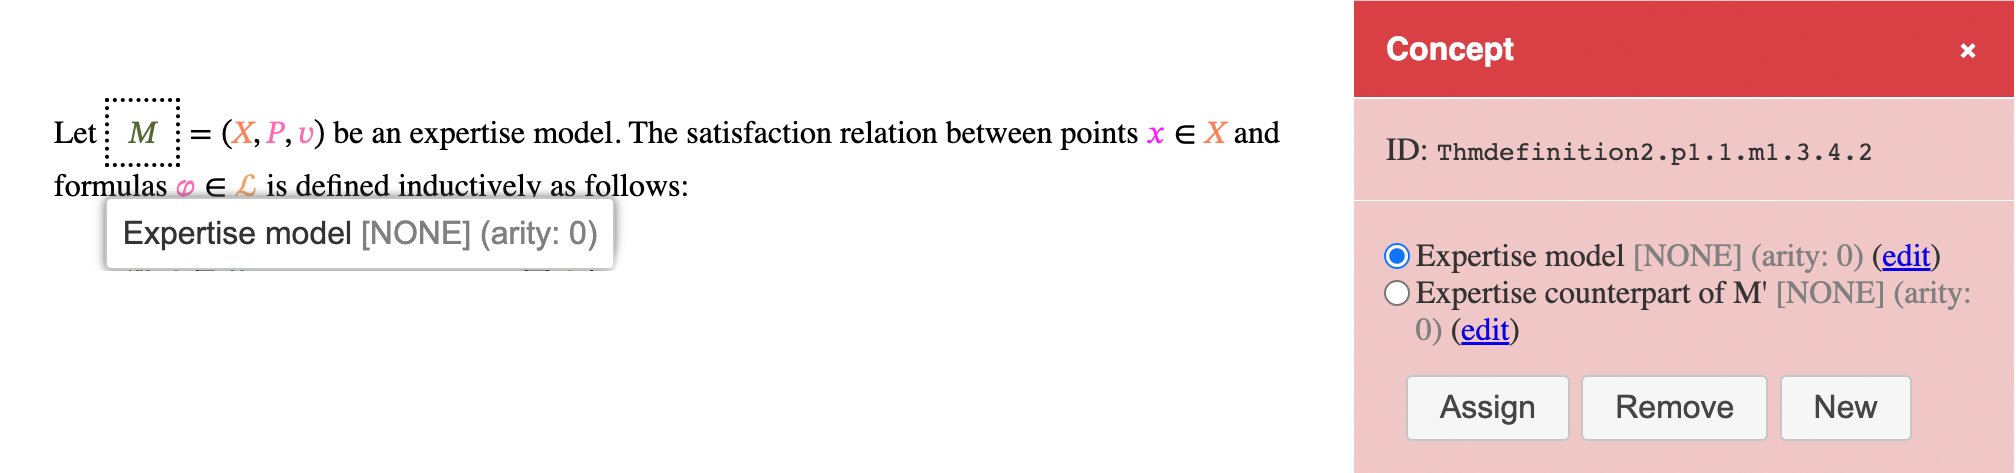
\includegraphics[width=14cm]{images/semantic-incorrectness.png}
  \end{tabular}
  \caption[Semantic Correctness]{Challenges in determining semantic correctness, where both the possible definitions look very similar but convey different meanings in a given context.}\label{fig:semantic-incorrectness}
\end{figure}

\chapter{Results}\label{chapter:results}

The outcomes of the annotation process using GPT and LLMs were compelling. GPT annotations exhibited superior quality and precision in explaining the identifiers. This chapter presents the results, including CoNLL scores, semantic accuracy scores, annotation costs, annotation duration, the extent of paper annotation by the LLMs, and the variance in scores due to the stochastic nature of LLMs.

\section{GPT}
We first scrutinised the annotations generated by GPT. For this analysis, we used all 40 papers from \cite{asakura2022building} as the ground truth and then employed GPT to generate dictionaries and annotations for all these papers.

\subsection{CoNLL Score}
The CoNLL score is a metric used to quantify the quality of coreference clusters. We obtained the weighted average of the CoNLL score across all the papers, with the weighting factored against the total number of annotations in the paper. Higher scores indicate better performance. As shown in Table \ref{tab:conll-score}, GPT-4 outperformed the other models, while GPT-3.5 exhibited the lowest score.

\begin{table}[htpb]
  \centering
  \begin{tabular}{lrr}
    \hline
    Model & Score & Weighted Score \\
    \hline
    gpt (average) & 79.31 & 76.89 \\
    gpt-3.5-turbo & 78.51 & 75.93 \\
    gpt-3.5-turbo-16k & 79.28 & 76.67 \\
    gpt-4 & 80.15 & 78.08\\
    \hline
  \end{tabular}
  \caption[CoNLL Scores]{Weighted average of CoNLL Scores.}
  \label{tab:conll-score}
\end{table}


\subsection{Coverage of Annotation}
Another critical aspect of this research was to examine the extent of the paper that the LLMs could successfully annotate. We represent this coverage in Table \ref{tab:anno-percentage}. GPT-4 demonstrated the highest coverage, while GPT-3.5 had the least.

\begin{table}[htpb]
  \centering
  \begin{tabular}{lr}
    \hline
    Model & Coverage \\
    \hline
    gpt (average) & 90.57\% \\
    gpt-3.5-turbo & 90.64\% \\
    gpt-3.5-turbo-16k & 88.21\% \\
    gpt-4 & 92.87\% \\
    \hline
  \end{tabular}
  \caption[Total coverage]{coverage of the annotation of the papers achieved by GPT}
  \label{tab:anno-percentage}
\end{table}

\subsection{Semantic Accuracy}
Semantic accuracy provides a measure of the correctness of the annotations. We weighted it against the coverage to represent the total. Because of the extensive difficulty of manually reviewing semantic accuracy, we evaluated five carefully picked papers representing various low/high CoNLL scores and lengths. As shown in Table \ref{tab:semantic-accuracy}, GPT-4 again outperformed all the models by a significant margin. There were a few papers where GPT-4 achieved an astonishing 100\% semantic accuracy.

\begin{table}[htpb]
  \centering
  \begin{tabular}{lrr}
    \hline
    Model & Score & Weighted Score \\
    \hline
    gpt (average) & 88.19\% & 79.87\% \\
    gpt-3.5-turbo & 84.69\% & 76.76\% \\
    gpt-3.5-turbo-16k & 84.17\% & 74.25\% \\
    gpt-4 & 95.70\% & 88.88\% \\
    \hline
  \end{tabular}
  \caption[Semantic Accuracy]{Weighted average of semantic accuracy}
  \label{tab:semantic-accuracy}
\end{table}

\subsection{Variance of Data}
Given the inherent stochastic nature of these models, some variation can be expected across multiple iterations. To account for this, we conducted multiple runs of the experiment on the reference paper ArXiV ID: 2107.10832 \citep{singleton2021logic} and tabulated the resultant variance. These outcomes are displayed in Table \ref{tab:variance}.

\begin{table}[htpb]
  \centering
  \begin{tabular}{lrrrrr}
    \hline
    Model & Best & Worst & Mean & Median & Std. Deviation \\
    \hline
    gpt (average) & 86.75 & 83.21 & 84.58 & 84.18 & 1.55 \\
    gpt-3.5-turbo & 82.83 & 80.00 & 81.28 & 81.15 & 1.17 \\
    gpt-3.5-turbo-16k & 88.38 & 83.47 & 85.29 & 84.65 & 2.16 \\
    gpt-4 & 89.05 & 86.16 & 87.18 & 86.75 & 1.32 \\
    \hline
  \end{tabular}
  \caption[Statistics of variance]{Different CoNLL scores across four different runs}
  \label{tab:variance}
\end{table}

\subsection{Running Time and Costs}

The cost and time efficiency of the employed models are critical to the feasibility of our automated approach. Tables \ref{tab:time} and \ref{tab:cost} respectively present the average time required and average cost incurred in annotating mathematical identifiers across GPT versions. The pricing is listed on the OpenAI website\footnote{\url{https://openai.com/pricing}}. While GPT-3.5 emerged as the fastest and most time-efficient model, the GPT-4 version manifested as the most costly. The relative cost per concept has been described in Table \ref{tab:relative-cost}

\begin{table}[htpb]
  \centering
  \begin{tabular}{lrrr}
    \hline
    Model & Dictionary Generation Time & Annotation Time & Total Time \\
    \hline
    gpt (average) & 03:49 & 03:25 & 07:14 \\
    gpt-3.5-turbo & 02:00 & 02:47 & 04:48 \\
    gpt-3.5-turbo-16k & 08:07 & 02:45 & 10:52 \\
    gpt-4 & 01:19 & 04:43 & 06:03 \\
    \hline
  \end{tabular}
  \caption[Average time taken]{Average time taken by each model (mm:ss)}
  \label{tab:time}
\end{table}

\begin{table}[htpb]
  \centering
  \begin{tabular}{lrr}
    \hline
    Model & Cost & Cost / 1M Tokens \\
    \hline
    gpt (average) & 1.80 & 9.415 \\
    gpt-3.5-turbo & 0.30 & 1.525 \\
    gpt-3.5-turbo-16k & 0.52 & 2.299 \\
    gpt-4 & 4.59 & 30.449 \\
    \hline
  \end{tabular}
  \caption[Cost Analysis]{Average cost of automation by each model in USD}
  \label{tab:cost}
\end{table}

\begin{table}[htpb]
  \centering
  \begin{tabular}{lrr}
    \hline
    Model & Cost / 1000 Concepts (USD) & Time / Concept (seconds) \\
    \hline
    gpt (average) & 2.49 & 0.73\\
    gpt-3.5-turbo & 0.40 & 0.46 \\
    gpt-3.5-turbo-16k & 0.88 & 1.25 \\
    gpt-4 & 6.18 & 0.47 \\
    \hline
  \end{tabular}
  \caption[Cost Analysis]{Relative cost and time taken}
  \label{tab:relative-cost}
\end{table}


\section{Open Source LLMs}
Upon successfully leveraging GPT to automate formula grounding, we proceeded to automate the process using Open Source Models. We applied the same metrics to see how they compete against GPT. The results were again impressive. Due to open-source LLMs' relatively slow speed and high running costs, we selected a subset of 7 papers out of the original 40 by \citet{asakura2022building}. We carefully chose the papers to cover a range of attributes, including high/low CoNLL scores, high/low semantic accuracy, and varied lengths.

\subsection{CoNLL Score}
We applied the same metrics of CoNLL score to the seven selected papers annotated by Open Source LLMs. We compared them against those annotated by GPT, with the human-annotated versions serving as the reference/ground truth. The values can be seen in Table \ref{tab:open-source-conll-score}. Among the open-source models, StableBeluga2 matched the performance of GPT models, indicating its commendable competence in creating high-quality coreference clusters. Vicuna-33b failed to annotate one paper entirely and has a score of 0.

\begin{table}[htpb]
  \centering
  \begin{tabular}{lrr}
    \hline
    Model & Score & Weighted Score \\
    \hline
    vicuna-33b & 72.44 & 77.45 \\
    gpt (average) & 88.75 & 87.55 \\
    gpt-3.5-turbo & 88.21 & 86.22 \\
    gpt-3.5-turbo-16k & 90.12 & 89.40 \\
    gpt-4 & 87.92 & 87.03 \\
    StableBeluga2 & 84.55 & 81.63 \\
    \hline
  \end{tabular}
  \caption[CoNLL Scores]{Weighted average of CoNLL Scores.}
  \label{tab:open-source-conll-score}
\end{table}


\subsection{Coverage of Annotation}
Open Source models also demonstrated impressive performance in their ability to annotate the papers. The values can be seen in Table \ref{tab:open-coverage}. StableBeluga2 had near-identical performance to the GPT Models. Vicuna-33b failed to annotate one paper entirely and has a score of 0.

\begin{table}[htpb]
  \centering
  \begin{tabular}{lr}
    \hline
    Model & Coverage \\
    \hline
    vicuna-33b & 66.18\% \\
    gpt (average) & 91.97\% \\
    gpt-3.5-turbo & 88.93\% \\
    gpt-3.5-turbo-16k & 90.62\% \\
    gpt-4 & 96.35\% \\
    StableBeluga2 & 93.17\% \\
    \hline
  \end{tabular}
  \caption[Total coverage]{coverage of the annotation of the papers achieved by GPT}
  \label{tab:open-coverage}
\end{table}

\subsection{Semantic Accuracy}
For semantic accuracy, we excluded one paper (ArXiV ID: 2107.10832 \citep{singleton2021logic}) due to its length. It was not feasible to manually evaluate it semantically due to its extensive length. We weighted the results against the coverage again to represent the total. As detailed in Table \ref{tab:open-semantic-accuracy}, the semblance between the performance of StableBeluga2 and GPT models reinforces this open-source model's potential in accurately understanding and reflecting the context of scientific papers.

\begin{table}[htpb]
  \centering
  \begin{tabular}{lrr}
    \hline
    Model & Score & Weighted Score \\
    \hline
    vicuna-33b & 61.58\% & 40.75\% \\
    gpt (average) & 88.19\% & 81.11\% \\
    gpt-3.5-turbo & 84.69\% & 75.31\% \\
    gpt-3.5-turbo-16k & 84.17\% & 76.27\% \\
    gpt-4 & 95.70\% & 92.21\% \\
    StableBeluga2 & 90.91\% & 84.70\% \\
    \hline
  \end{tabular}
  \caption[Semantic Accuracy]{Weighted average of semantic accuracy}
  \label{tab:open-semantic-accuracy}
\end{table}

\subsection{Variance of Data}
It was impossible to calculate the data variance due to the high costs of running the Open Source Models and budget constraints. However, preliminary testing during the model selection phase indicated that Open Source Models were considerably more stable than GPT.

\subsection{Running Time and Costs}
Given the distinctive operational requirements of open-source models, the computation of time and cost efficiencies differ from those of GPT models. Unlike GPT models, the cost for open-source models revolves around GPU runtime on the servers of \href{https://runpod.io}{runpod.io} and not token usage. Table \ref{tab:open-time} and \ref{tab:open-cost} represent these essential aspects. The pricing of GPT is listed on the OpenAI website\footnote{\url{https://openai.com/pricing}}. The cost of running vicuna-33b was 0.69USD/h, and StableBeluga2 was 1.84USD/h.

\begin{table}[htpb]
  \centering
  \begin{tabular}{lrrr}
    \hline
    Model & Dictionary Generation Time & Annotation Time & Total Time \\
    \hline
    vicuna-33b & 04:16 & 07:16 & 12:33 \\
    gpt (average) & 01:54 & 01:53 & 03:48 \\
    gpt-3.5-turbo & 01:04 & 01:21 & 02:25 \\
    gpt-3.5-turbo-16k & 04:02 & 02:18 & 06:21 \\
    gpt-4 & 00:38 & 02:01 & 02:39 \\
    StableBeluga2 & 05:17 & 09:43 & 20:20 \\
    \hline
  \end{tabular}
  \caption[Average time taken]{Average time taken by each model (mm:ss)}
  \label{tab:open-time}
\end{table}

\begin{table}[htpb]
  \centering
  \begin{tabular}{lrrr}
    \hline
    Model & Cost & Cost / 1000 Concepts (USD) & Time / Concept (seconds) \\
    \hline
    vicuna-33b & 0.14 & 0.51 & 2.73 \\
    gpt (average) & 1.80 & 2.70 & 1.06 \\
    gpt-3.5-turbo & 0.15 & 0.43 & 0.60 \\
    gpt-3.5-turbo-16k & 0.22 & 1.01 & 2.10 \\
    gpt-4 & 2.06 & 6.67 & 0.48 \\
    StableBeluga2 & 0.62 & 2.77 & 5.48 \\
    \hline
  \end{tabular}
  \caption[Cost Analysis]{Average cost of annotation by each model}
  \label{tab:open-cost}
\end{table}

\chapter{Analysis}\label{chapter:analysis}

This chapter embarks on a thorough and incisive exploration of the results obtained, elucidating the significance of the observed scores and probing into the reasons behind their variation. This analysis examines the CoNLL scores, semantic accuracy scores, annotation costs, annotation duration, extent of paper annotation by the LLMs, and the variance in scores due to the stochastic nature of LLMs. While specific observations, such as the superior performance of models with more parameters, might appear intuitive, the analysis also uncovers less apparent insights.

\section{GPT}
The analysis commenced with examining the annotations generated by three variations of the GPT model: GPT-3.5, GPT-3.5-16k, and GPT-4. The ground truth was derived from 40 papers penned by \citet{asakura2022building}, and these were utilised as templates for GPT-generated dictionaries and annotations. An emerging pattern in these results showcased GPT-4 as a starkly superior model compared to GPT-3.5-16k and GPT-3.5. 

\subsection{CoNLL Score}
The CoNLL score measures the quality of coreference clusters, employing a weighted average to keep the vast number of annotations in check. The CoNLL Scores of all three models are presented illustratively in Figure \ref{fig:violin-conll}, with GPT-4 demonstrating visibly superior and more consistent results than its counterparts.

\begin{figure}[htpb]
  \centering
  \begin{tabular}{c}
  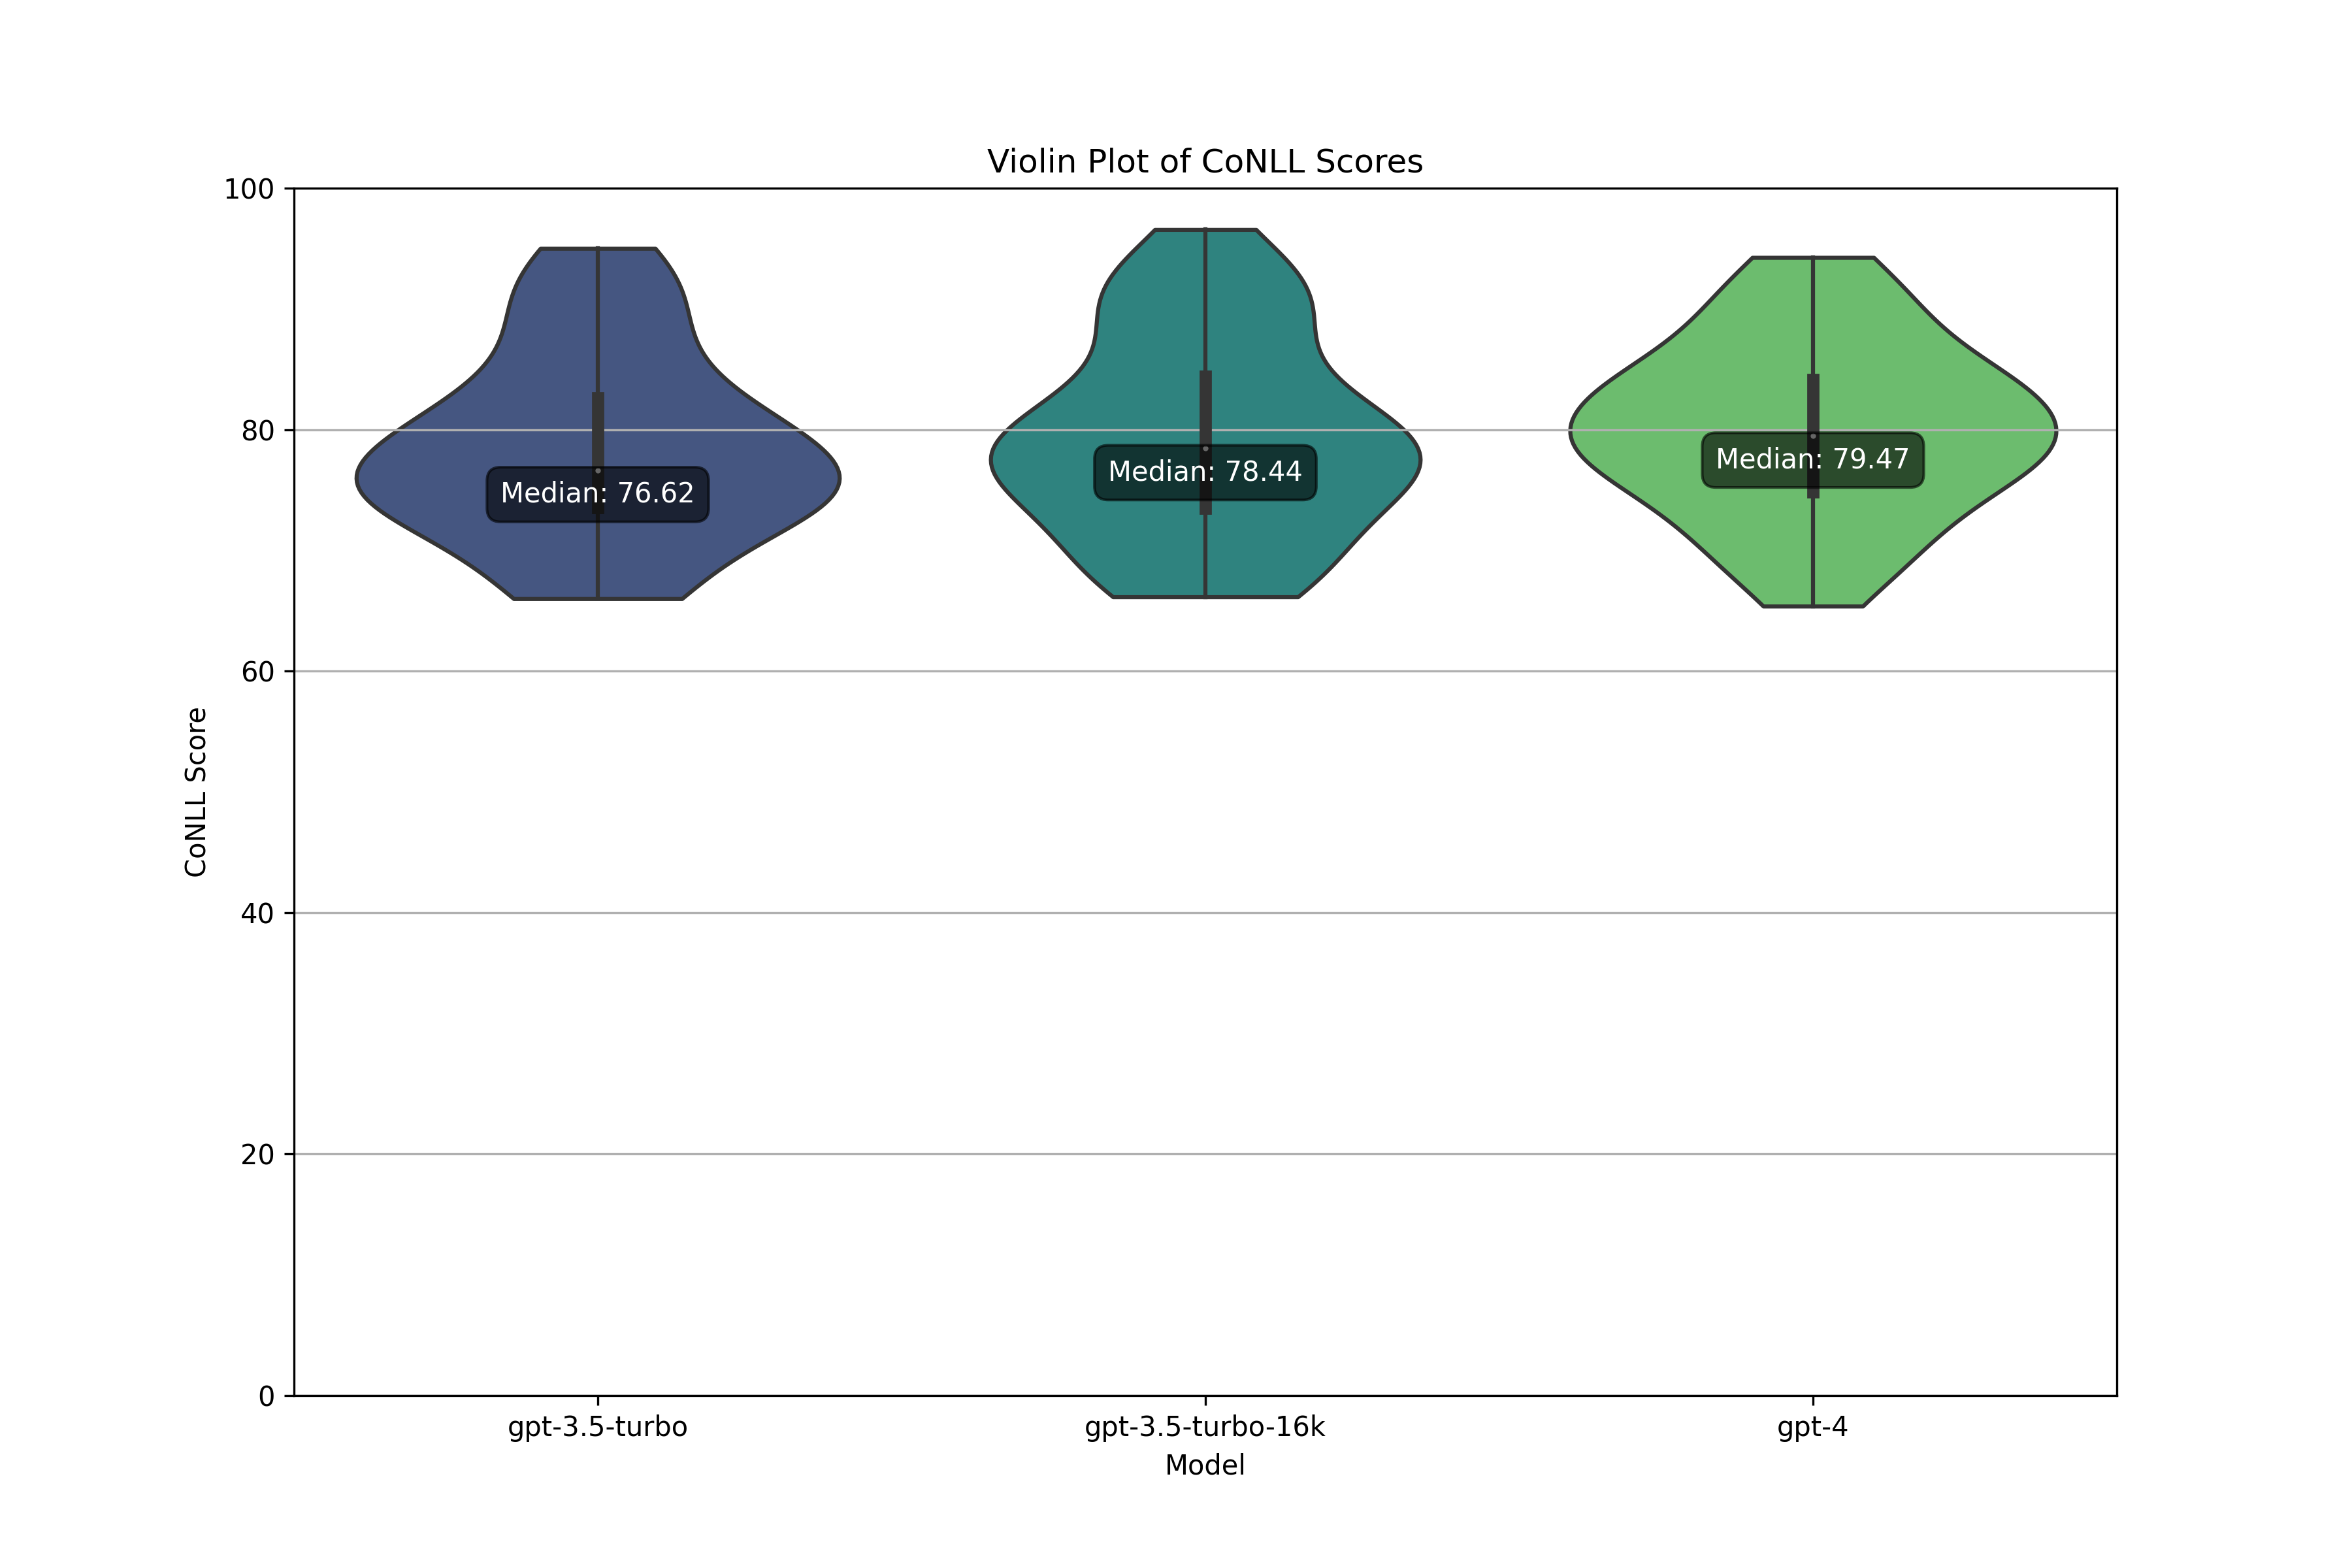
\includegraphics[width=14cm]{images/conll-score.png}
  \end{tabular}
  \caption[Distribution of CoNLL Score]{Violin Plot of CoNLL Score of all three different models}\label{fig:violin-conll}
\end{figure}

\subsection{Estimation of CoNLL Score}
Our deductions present that the computation of the CoNLL score is contingent upon four primary factors: 
    \begin{enumerate}
        \item Model: The hierarchy is clear — GPT4 outshines GPT-3.5-16k, which in turn surpasses GPT-3.5. 
        \item Topic: Our experiments revealed that papers from specific disciplines performed better — Logic outpaced NLP, which was further ahead of Astronomy, with Mathematics trailing them all. The underlying reason for this is perhaps the training data. Due to the open nature of OpenAI, it is impossible to verify this claim. Moreover, the inherent nature of Language Models struggling with Mathematics is perhaps another reason GPT suffered in Mathematics papers.
        \item Ambiguity pertains to the total number of discrete identifiers in the given paper. It goes without saying that the lower the number of identifiers, the better a model typically performs, as there are fewer distinctions to make. For example, in the formula $x = \frac{-b \pm \sqrt{b^2 - 4ac}}{2a}$ there are 4 identifiers, $x$, $a$, $b$, and $c$.
        \item Obscurity: This is estimated using the interquartile range of a given identifier's occurrences, focusing solely on the middle quartile and disregarding the outliers. From the same example of the quadratic equation of $x = \frac{-b \pm \sqrt{b^2 - 4ac}}{2a}$, $x$ and $c$ are repeated once but $a$ and $b$ are repeated twice. The rationale for focusing on the middle 40th percentile range is twofold. First, due to their limited occurrences, identifiers that appear infrequently (in the bottom 30th percentile) are generally easier for GPT to disambiguate. Second, persistent identifiers (in the top 30th percentile) may challenge annotation. However, our annotation approach results in a cascading effect that minimises its impact on the CoNLL score. Therefore, the identifiers falling within the middle 40th percentile truly contribute to the level of Obscurity. This subset is the primary focus when estimating the CoNLL score for annotation accuracy.
    \end{enumerate}

These four variables help devise a robust mathematical formula to estimate the CoNLL score, with the computation process detailed in Figure \ref{fig:conll-estimation}. Despite the limited sample size, preliminary results in Table \ref{tab:mse-r2} demonstrate the potential of this predictive model.

\clearpage

\begin{figure}[htpb]
  \begin{equation}
      \text{estimated\_conll\_score} \simeq \frac{-2}{5} \times \text{total\_concepts} + \frac{-1}{5} \times \text{occur\_iqr} + \text{intercept}
  \end{equation}
  \caption[CoNLL Estimation]{Estimate the CoNLL Score for NLP Papers}
  \label{fig:conll-estimation}
\end{figure}

In the equation above, the variables are defined as follows:
\begin{itemize}
  \item \textbf{estimated\_conll\_score} is the estimated CoNLL score.
  \item \textbf{total\_concepts} is the total number of concepts in the paper (Ambiguity).
  \item \textbf{occur\_iqr} represents (Obscurity).
  \item \textbf{intercept} is the y-intercept which depends on the model. gpt-3.5 = 93, gpt-3.5-16k = 95, gpt-4 = 97.
\end{itemize}

Figure \ref{fig:esimated-conll} shows the visualisation of our novel formula on a 3D plane.

\begin{figure}[htpb]
  \centering
  \subfloat[Angled View]{
    \begin{tabular}{c}
  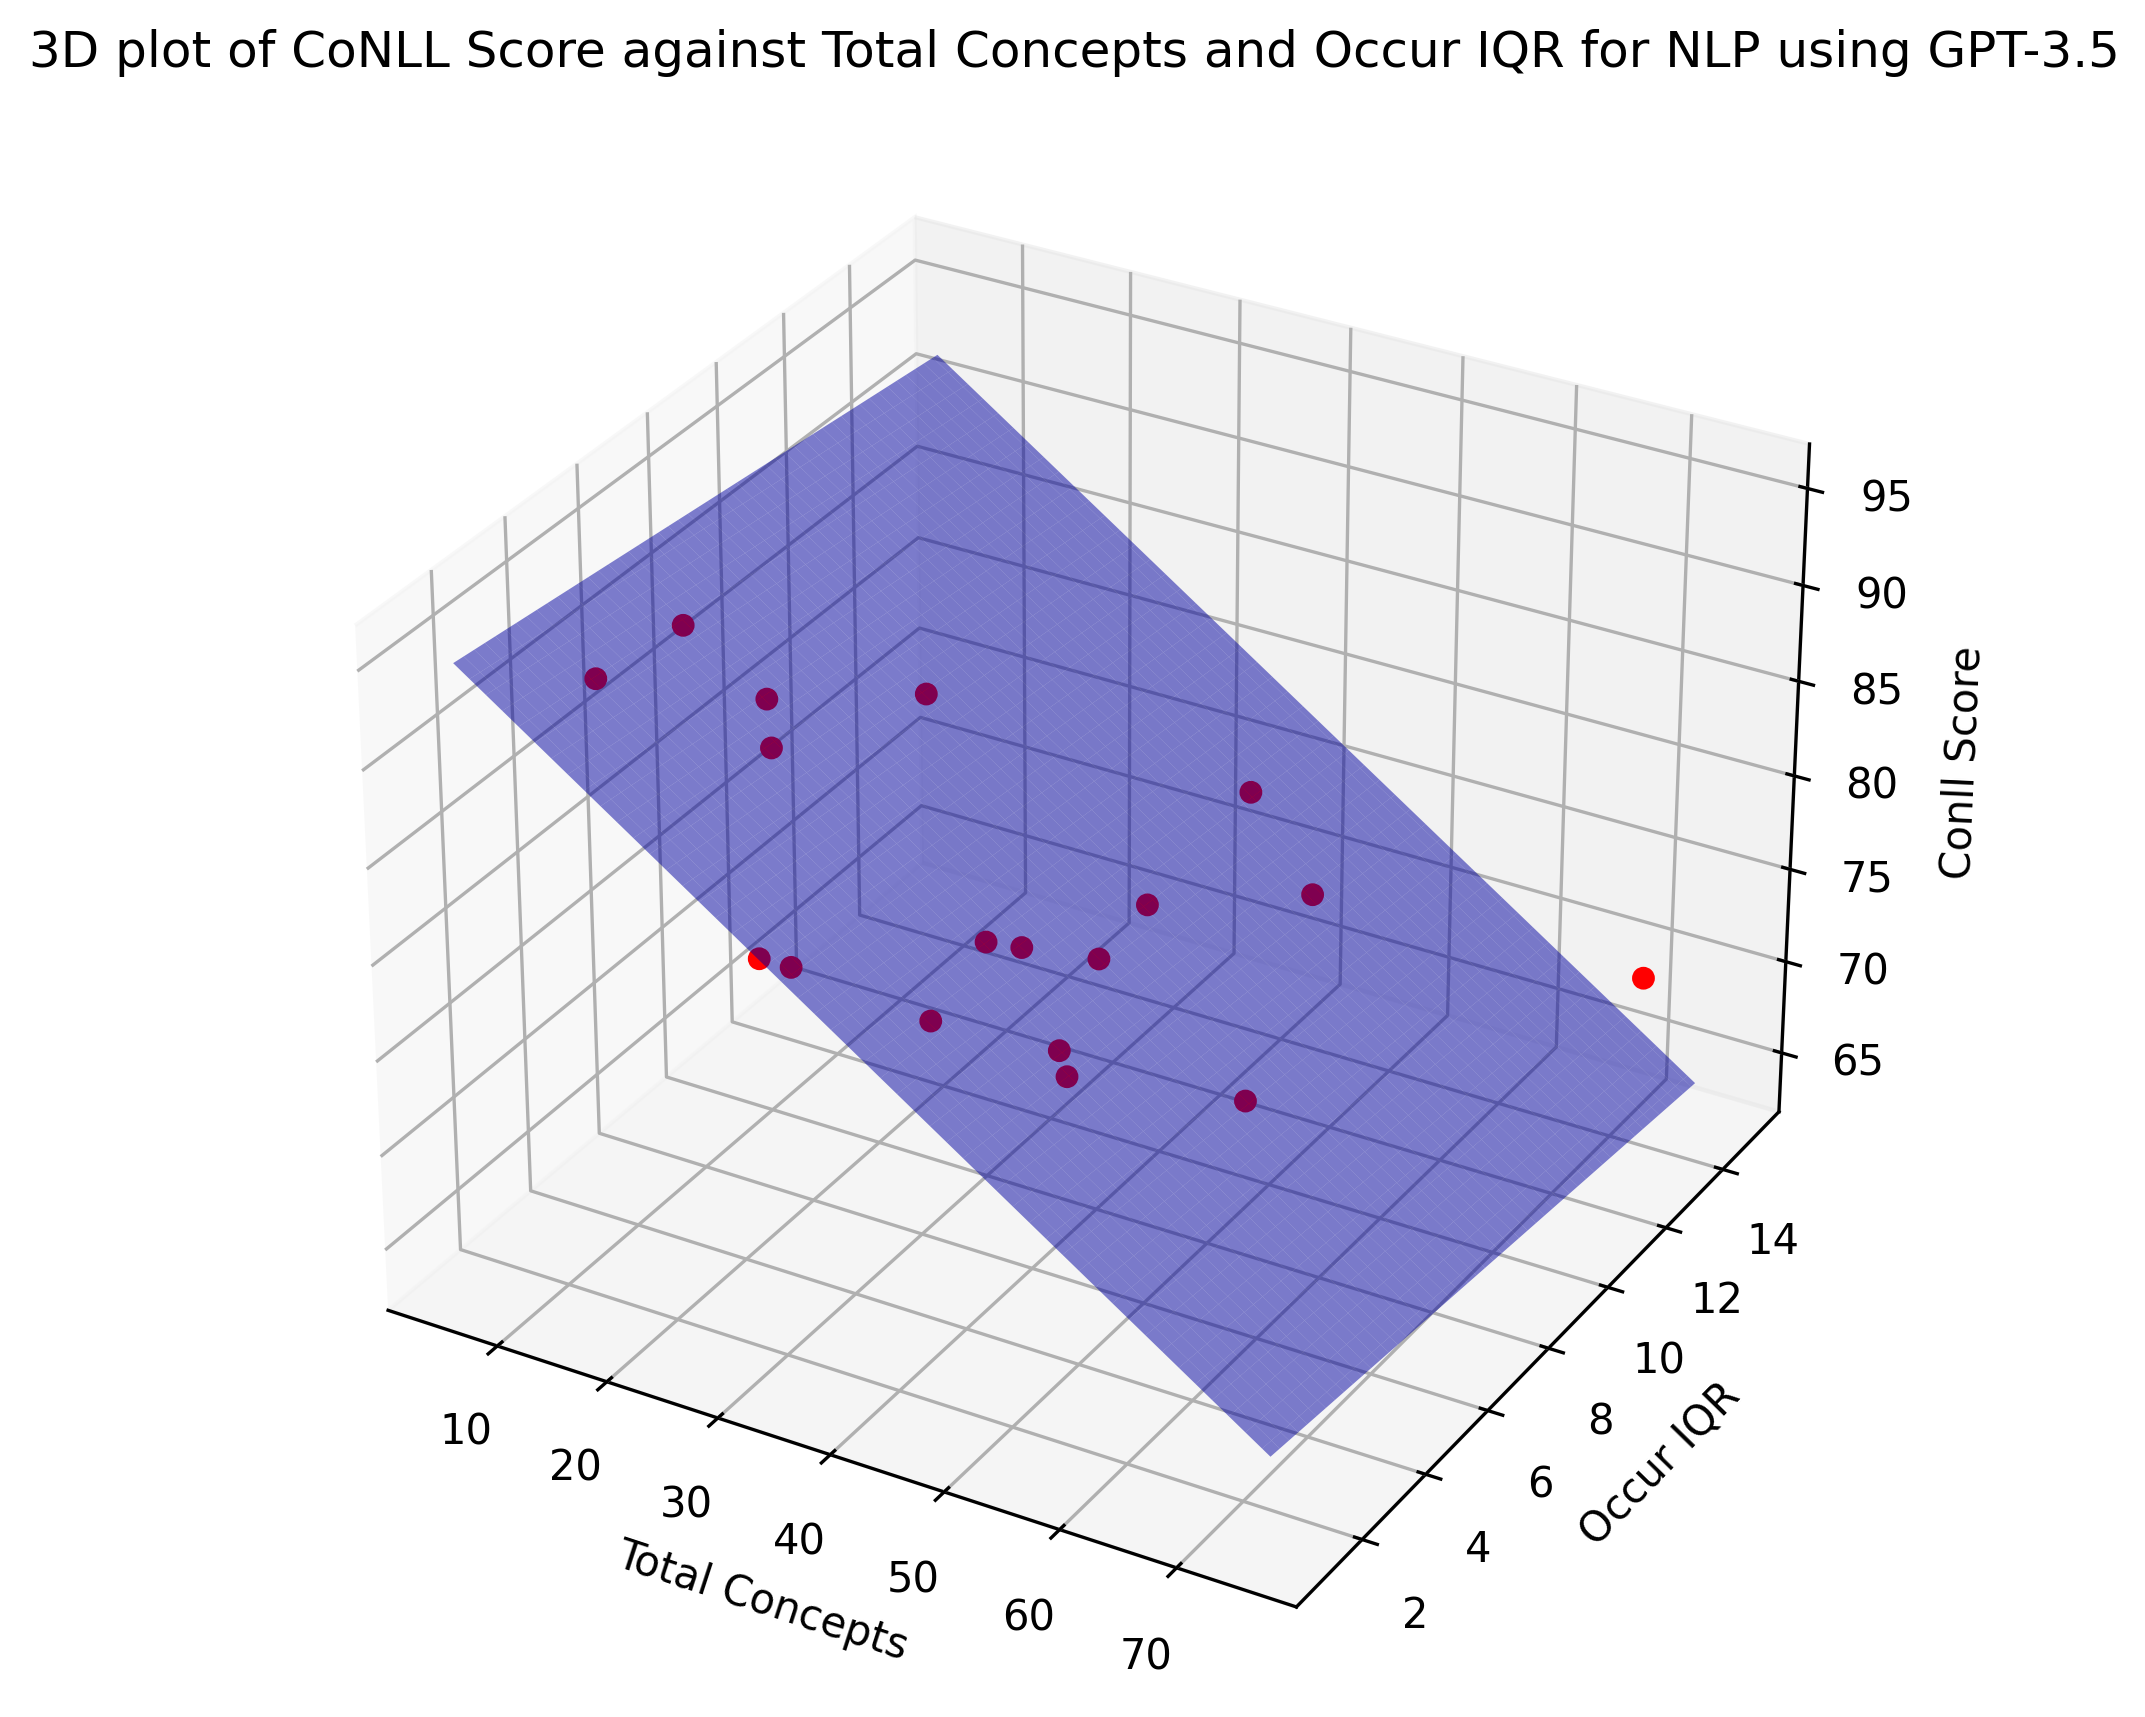
\includegraphics[width=11cm]{images/estimated-conll.png}
  \end{tabular}
  }
  \quad 
  \subfloat[Side view]{
    \begin{tabular}{c}
  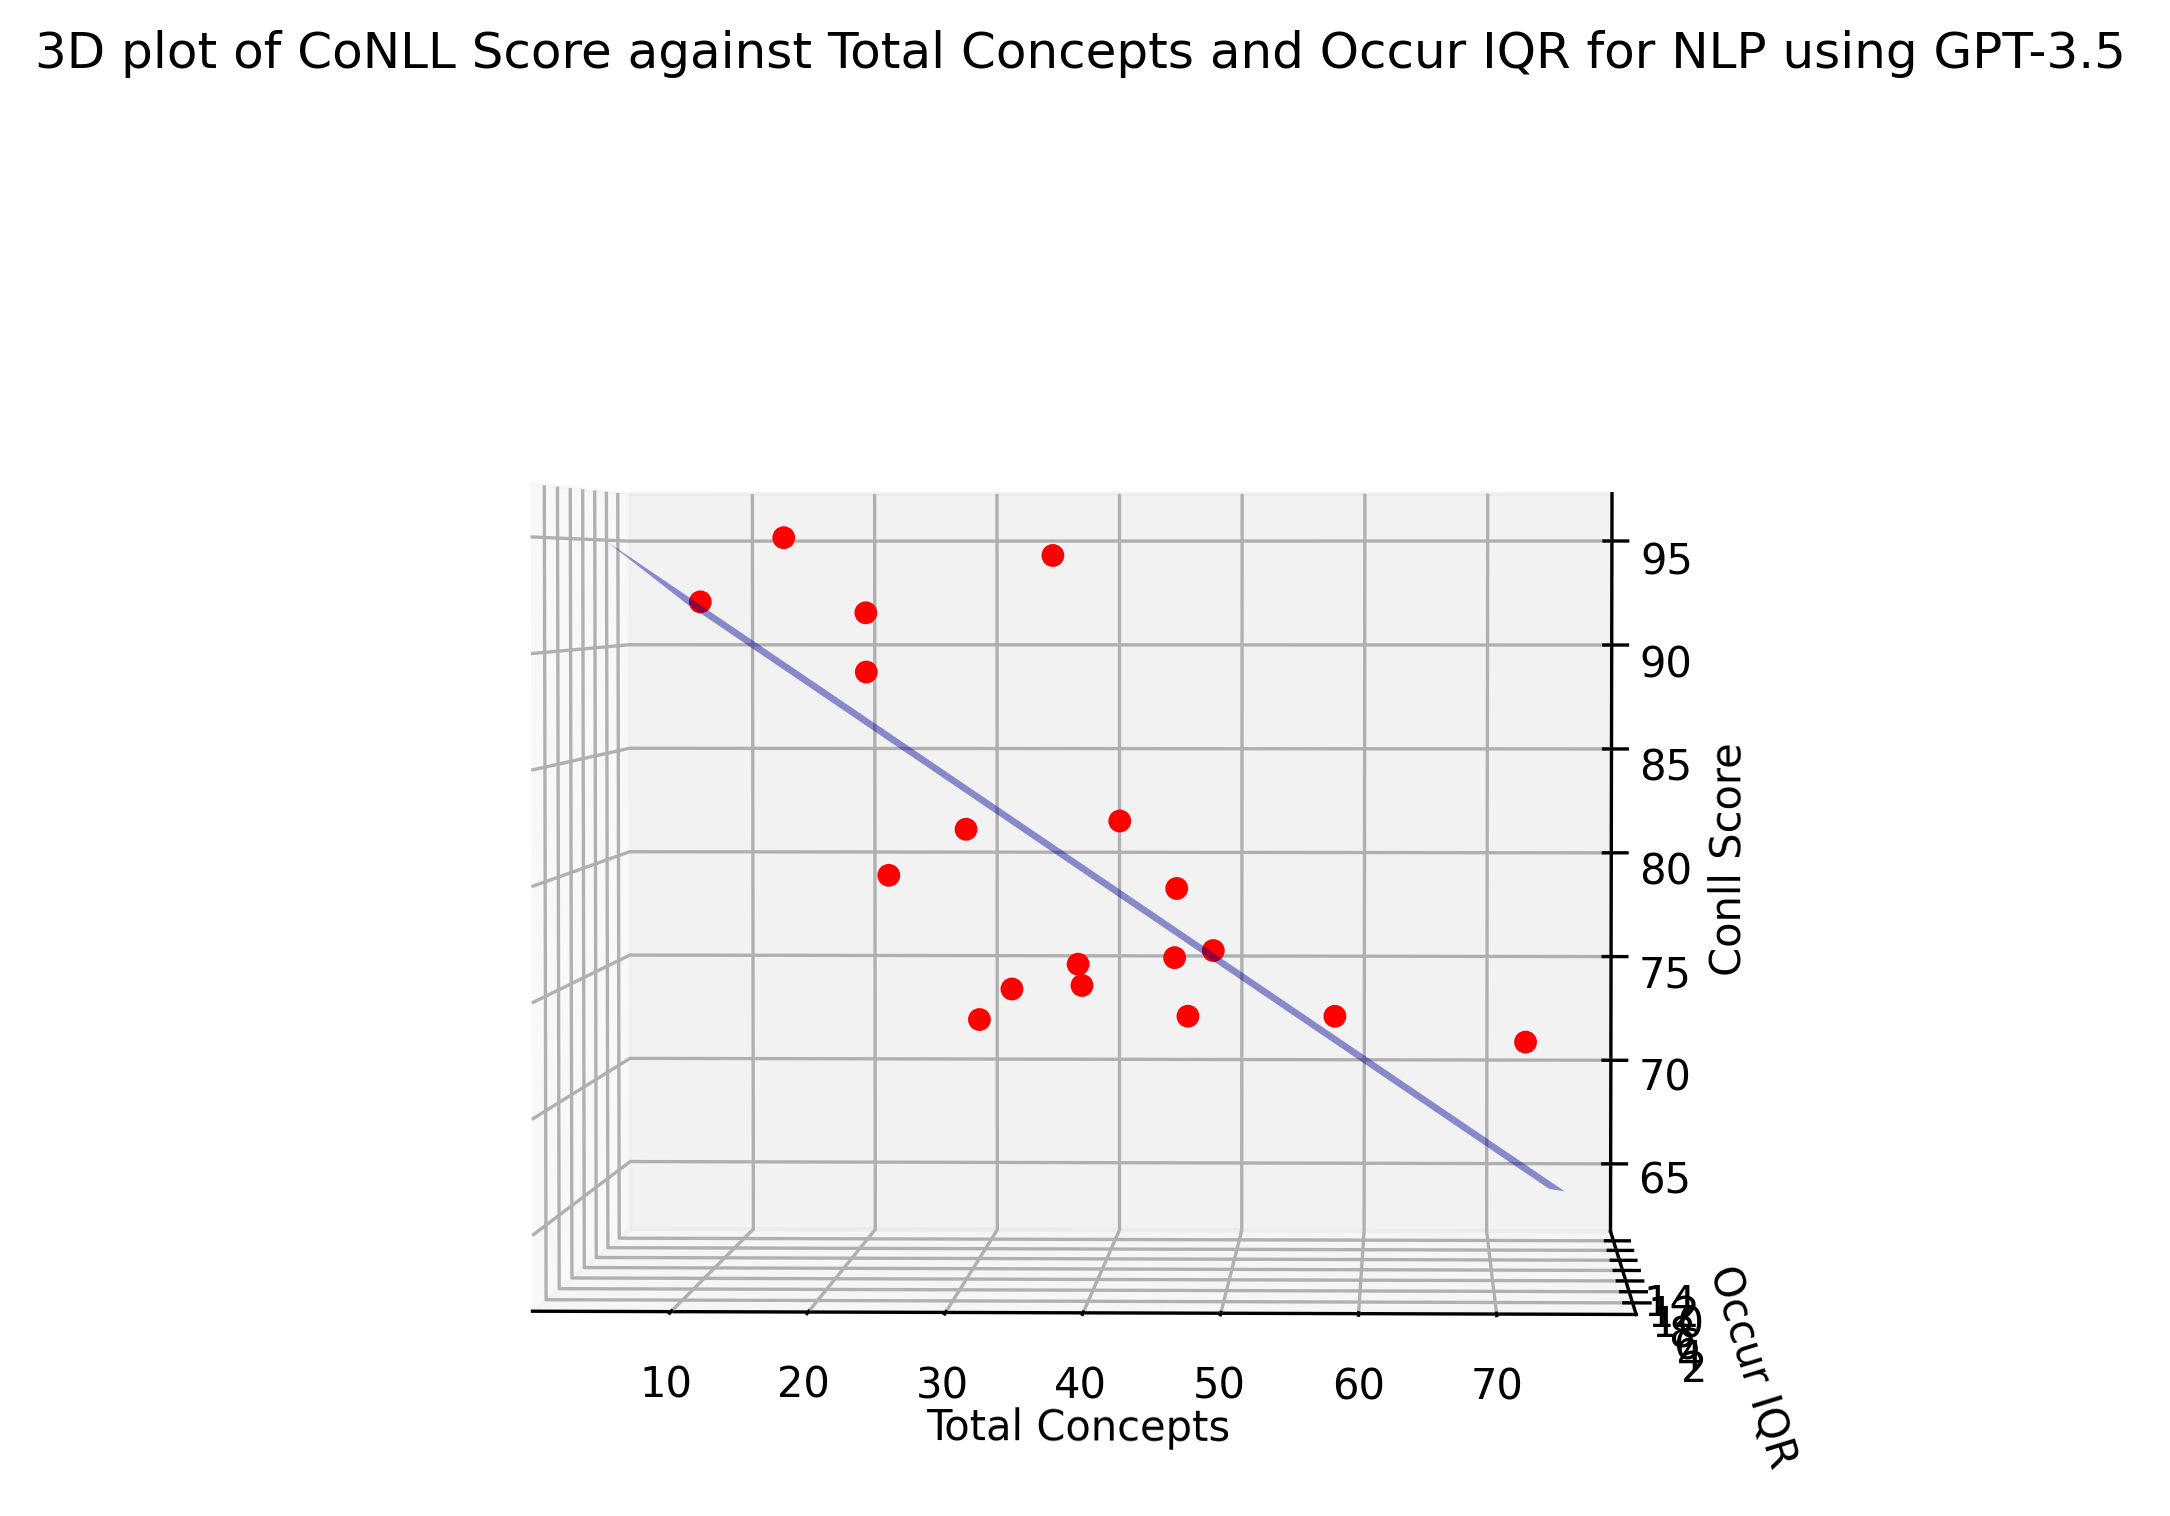
\includegraphics[width=11cm]{images/estimated-conll-2.png}
  \end{tabular}
  }
  \caption[CoNLL Score Estimation]{3D Visualisation of the CoNLL Score Estimation Formula}\label{fig:esimated-conll}
\end{figure}

Table \ref{tab:mse-r2} shows the estimation formula's Mean Square Error and R2 Score. Since there were only 18 papers in hand for NLP, getting better results was difficult.

\begin{table}[h]
    \centering
    \begin{tabular}{lrr}
        \hline
        Model & Mean Square Error & R2 Score \\
        \hline
        GPT-3.5-turbo & 35.636 & 0.136 \\
        GPT-3.5-16k-turbo & 25.936 & 0.371 \\
        GPT-4 & 26.386 & 0.360 \\
        \hline
    \end{tabular}
    \caption{Mean Square Error and R2 Score of the Estimation Formula}
    \label{tab:mse-r2}
\end{table}

\subsection{Coverage of Annotation}

The coverage of annotation refers to the proportion of the paper that the LLMs successfully annotated. Consistent with the CoNLL results, GPT-4 again made a mark by consistently outperforming the other two GPT models. GPT-3.5-16k, in contrast, had lesser coverage than GPT-3.5 due to the former's instability and propensity for repetition death. Figure \ref{fig:violin-coverage} provides a visual representation of the coverage exhibited by all three models.

\begin{figure}[htpb]
  \centering
  \begin{tabular}{c}
  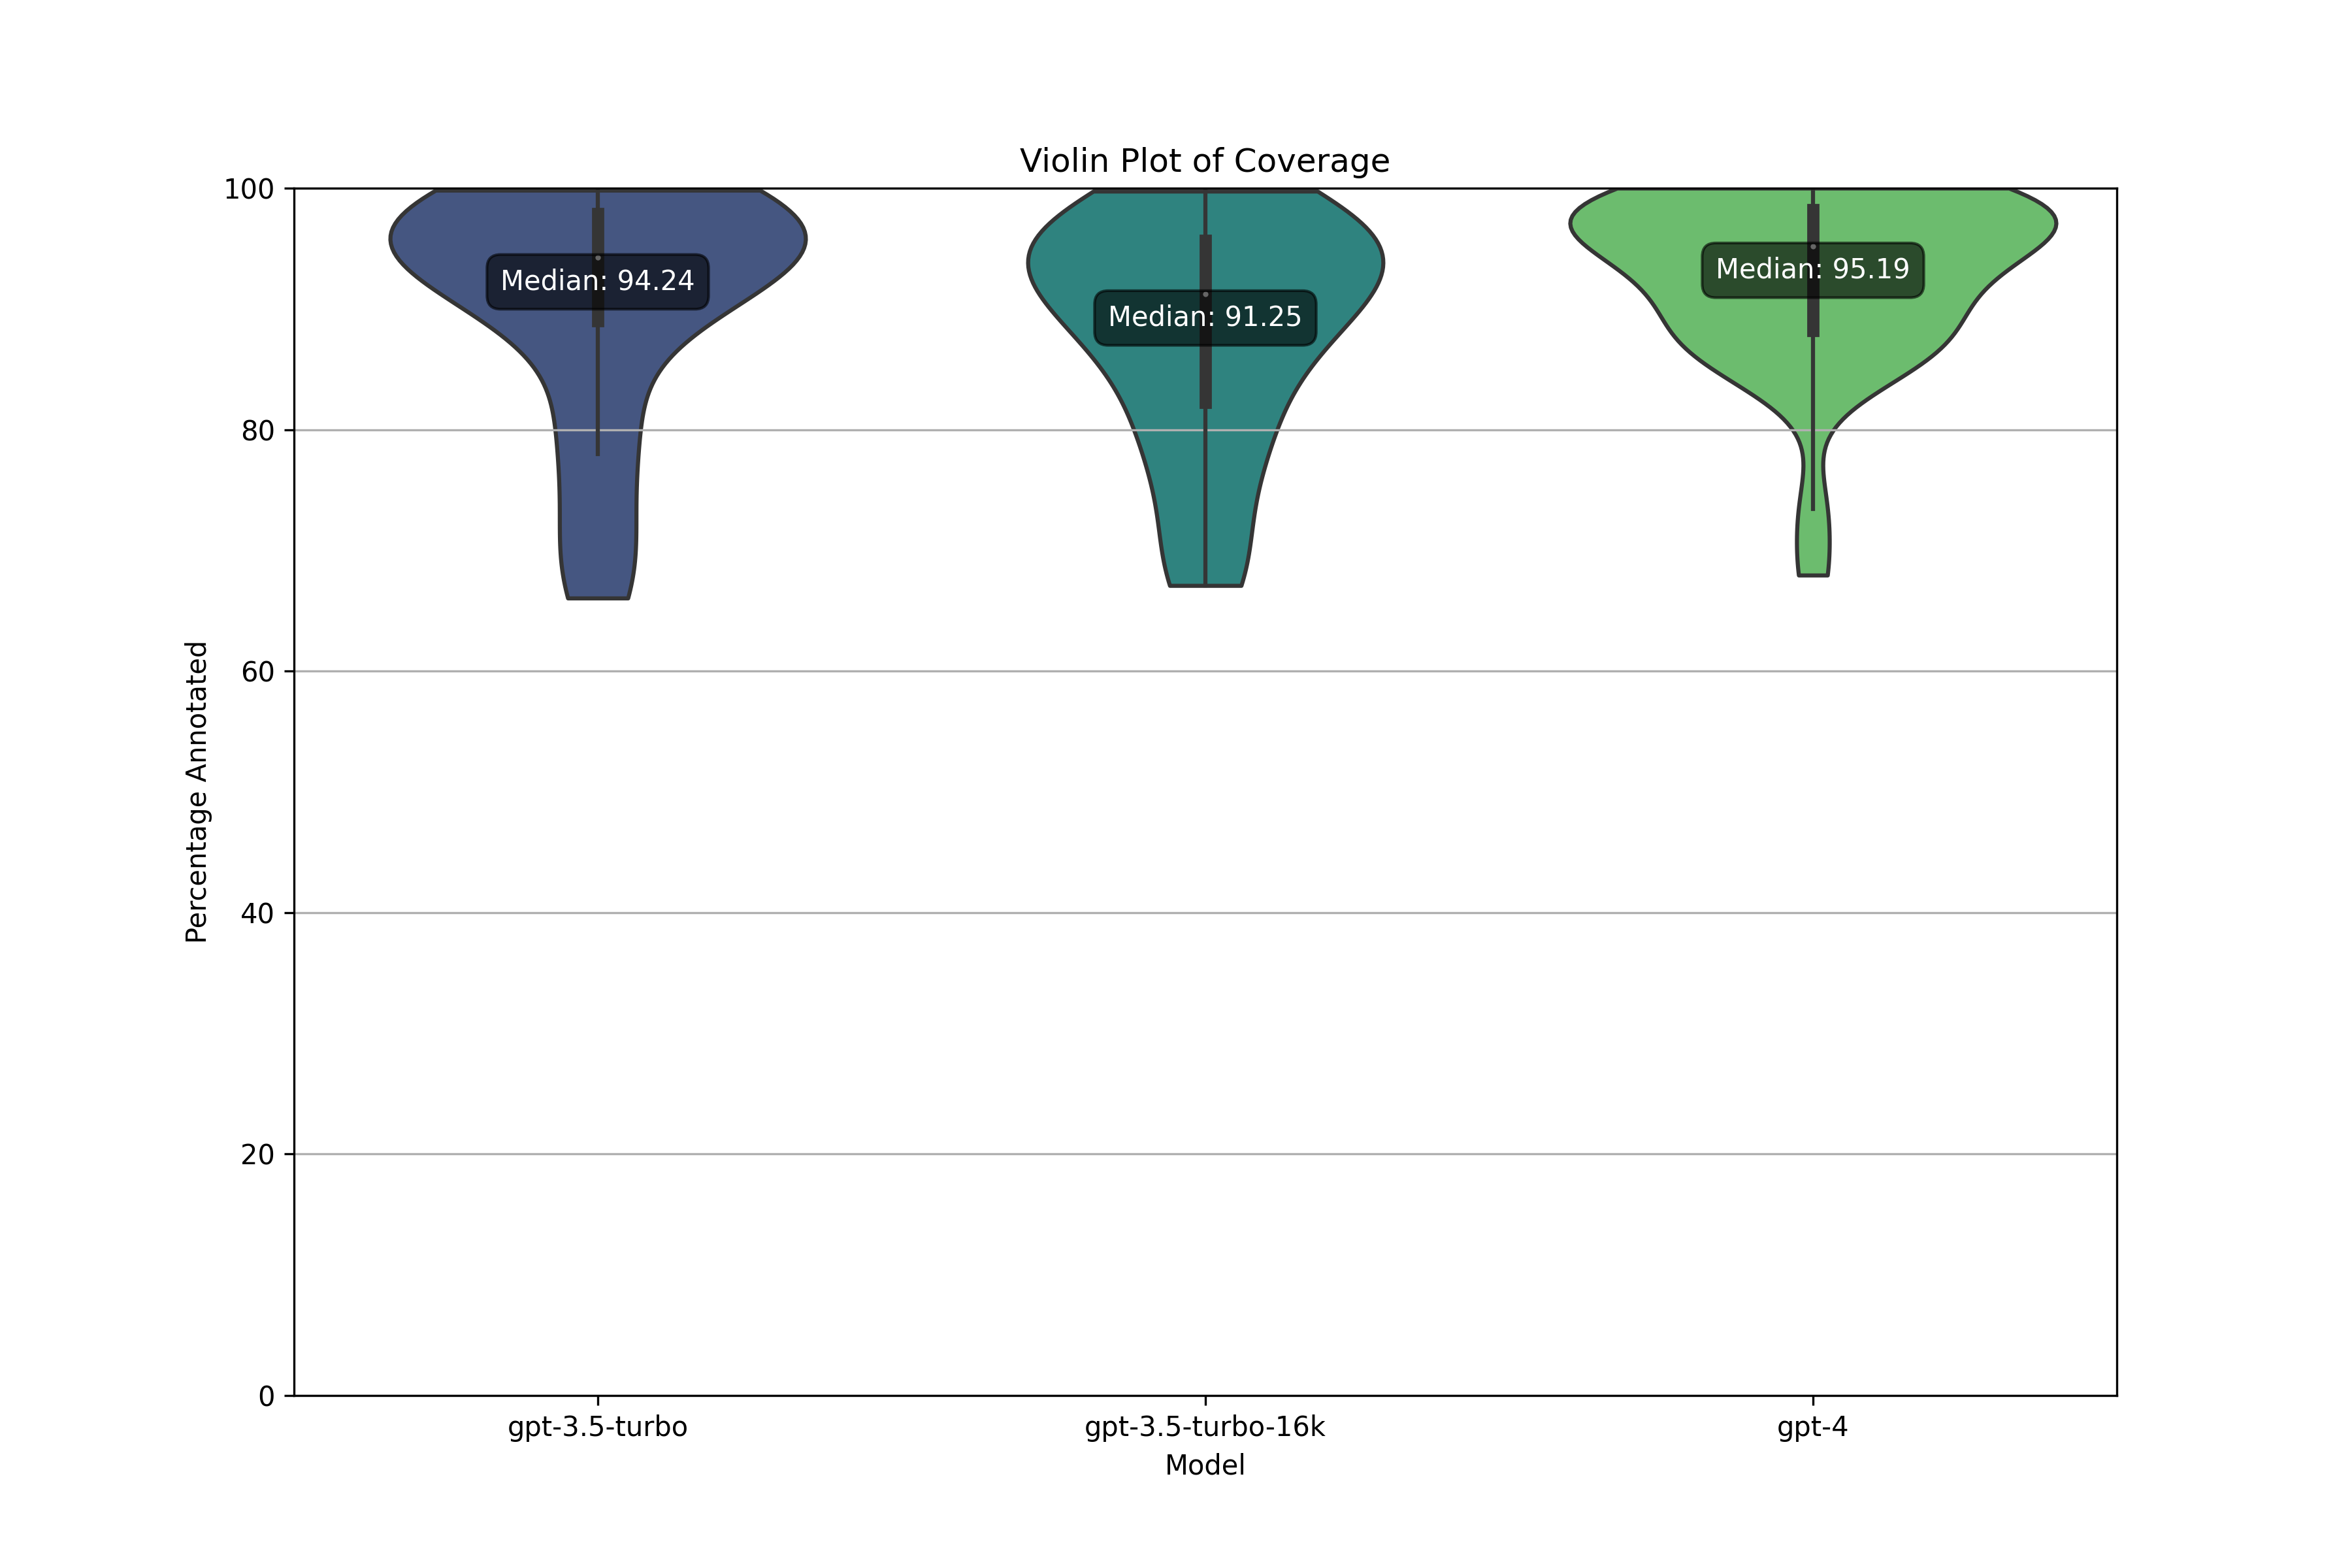
\includegraphics[width=14cm]{images/coverage.png}
  \end{tabular}
  \caption[Distribution of Coverage]{Violin Plot of the Coverage of Annotations of all three different models}\label{fig:violin-coverage}
\end{figure}
 
\subsection{Semantic Accuracy}

Semantic accuracy provides a measure of the correctness of the annotations. We weighted it against the coverage to represent the total. Because of the extensive difficulty of manually reviewing semantic accuracy, we evaluated five carefully picked papers representing various low/high CoNLL scores and lengths. As detailed in Figure \ref{fig:violin-semantic}, GPT-4 consistently outperformed all the other models by a significant margin. There were a few papers where GPT-4 achieved an astonishing 100\% semantic accuracy, but weighing it with coverage brings it down to 98\%. GPT-4's worst performance is almost as good as the best performances of other models, marking it as superior. This comes as no surprise as GPT-4 is one of the largest LLMs as of writing this thesis.

\begin{figure}[htpb]
  \centering
  \begin{tabular}{c}
  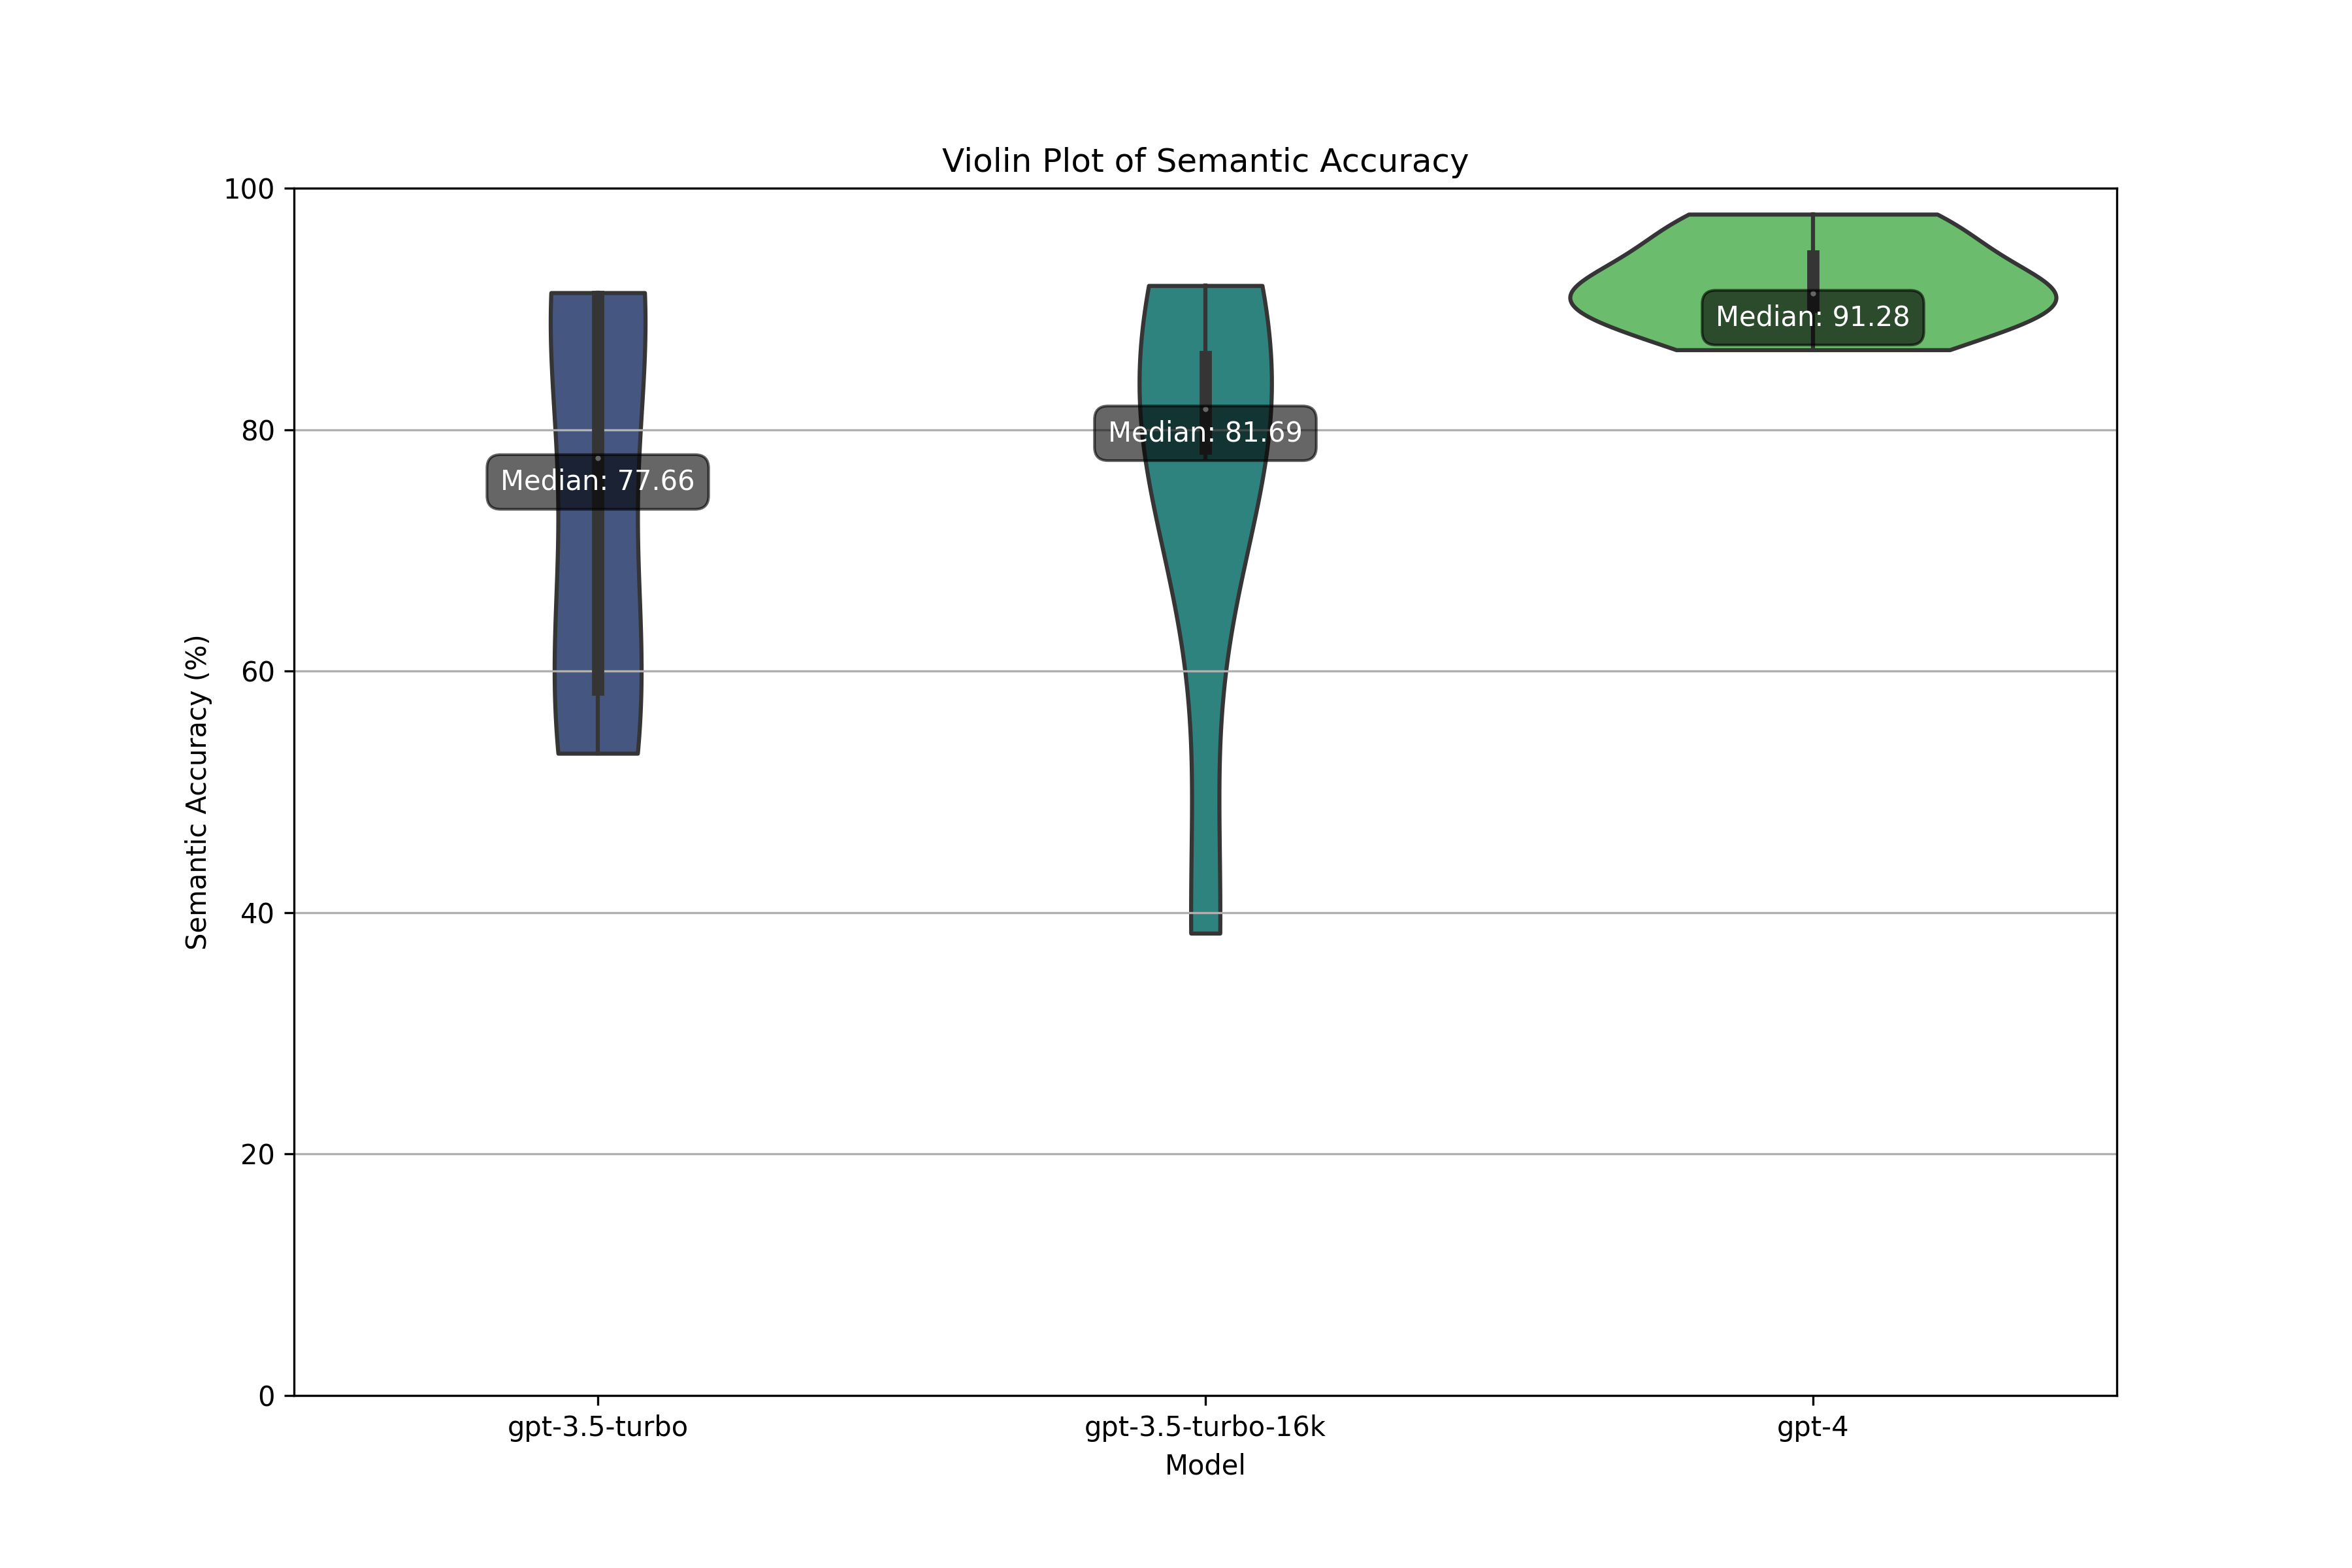
\includegraphics[width=14cm]{images/semantic-accuracy.png}
  \end{tabular}
  \caption[Semantic Accuracy]{Violin Plot of the Weighted Semantic Accuracy of all GPT Models}\label{fig:violin-semantic}
\end{figure}

\subsection{Variance of Data}

To account for these models' stochastic nature and ensure our experiment's reproducibility and stability, we sampled one reference paper, ArXiV ID: 2107.10832 \citep{singleton2021logic}. We ran the experiment four times, evaluating the variance in the CoNLL scores. GPT-3.5 and GPT-4 proved monumentally stable, whereas GPT-3.5-16k, a newer model, still exhibited volatility issues. These outcomes are displayed in Figure \ref{fig:violin-variance}.

\begin{figure}[htpb]
  \centering
  \begin{tabular}{c}
  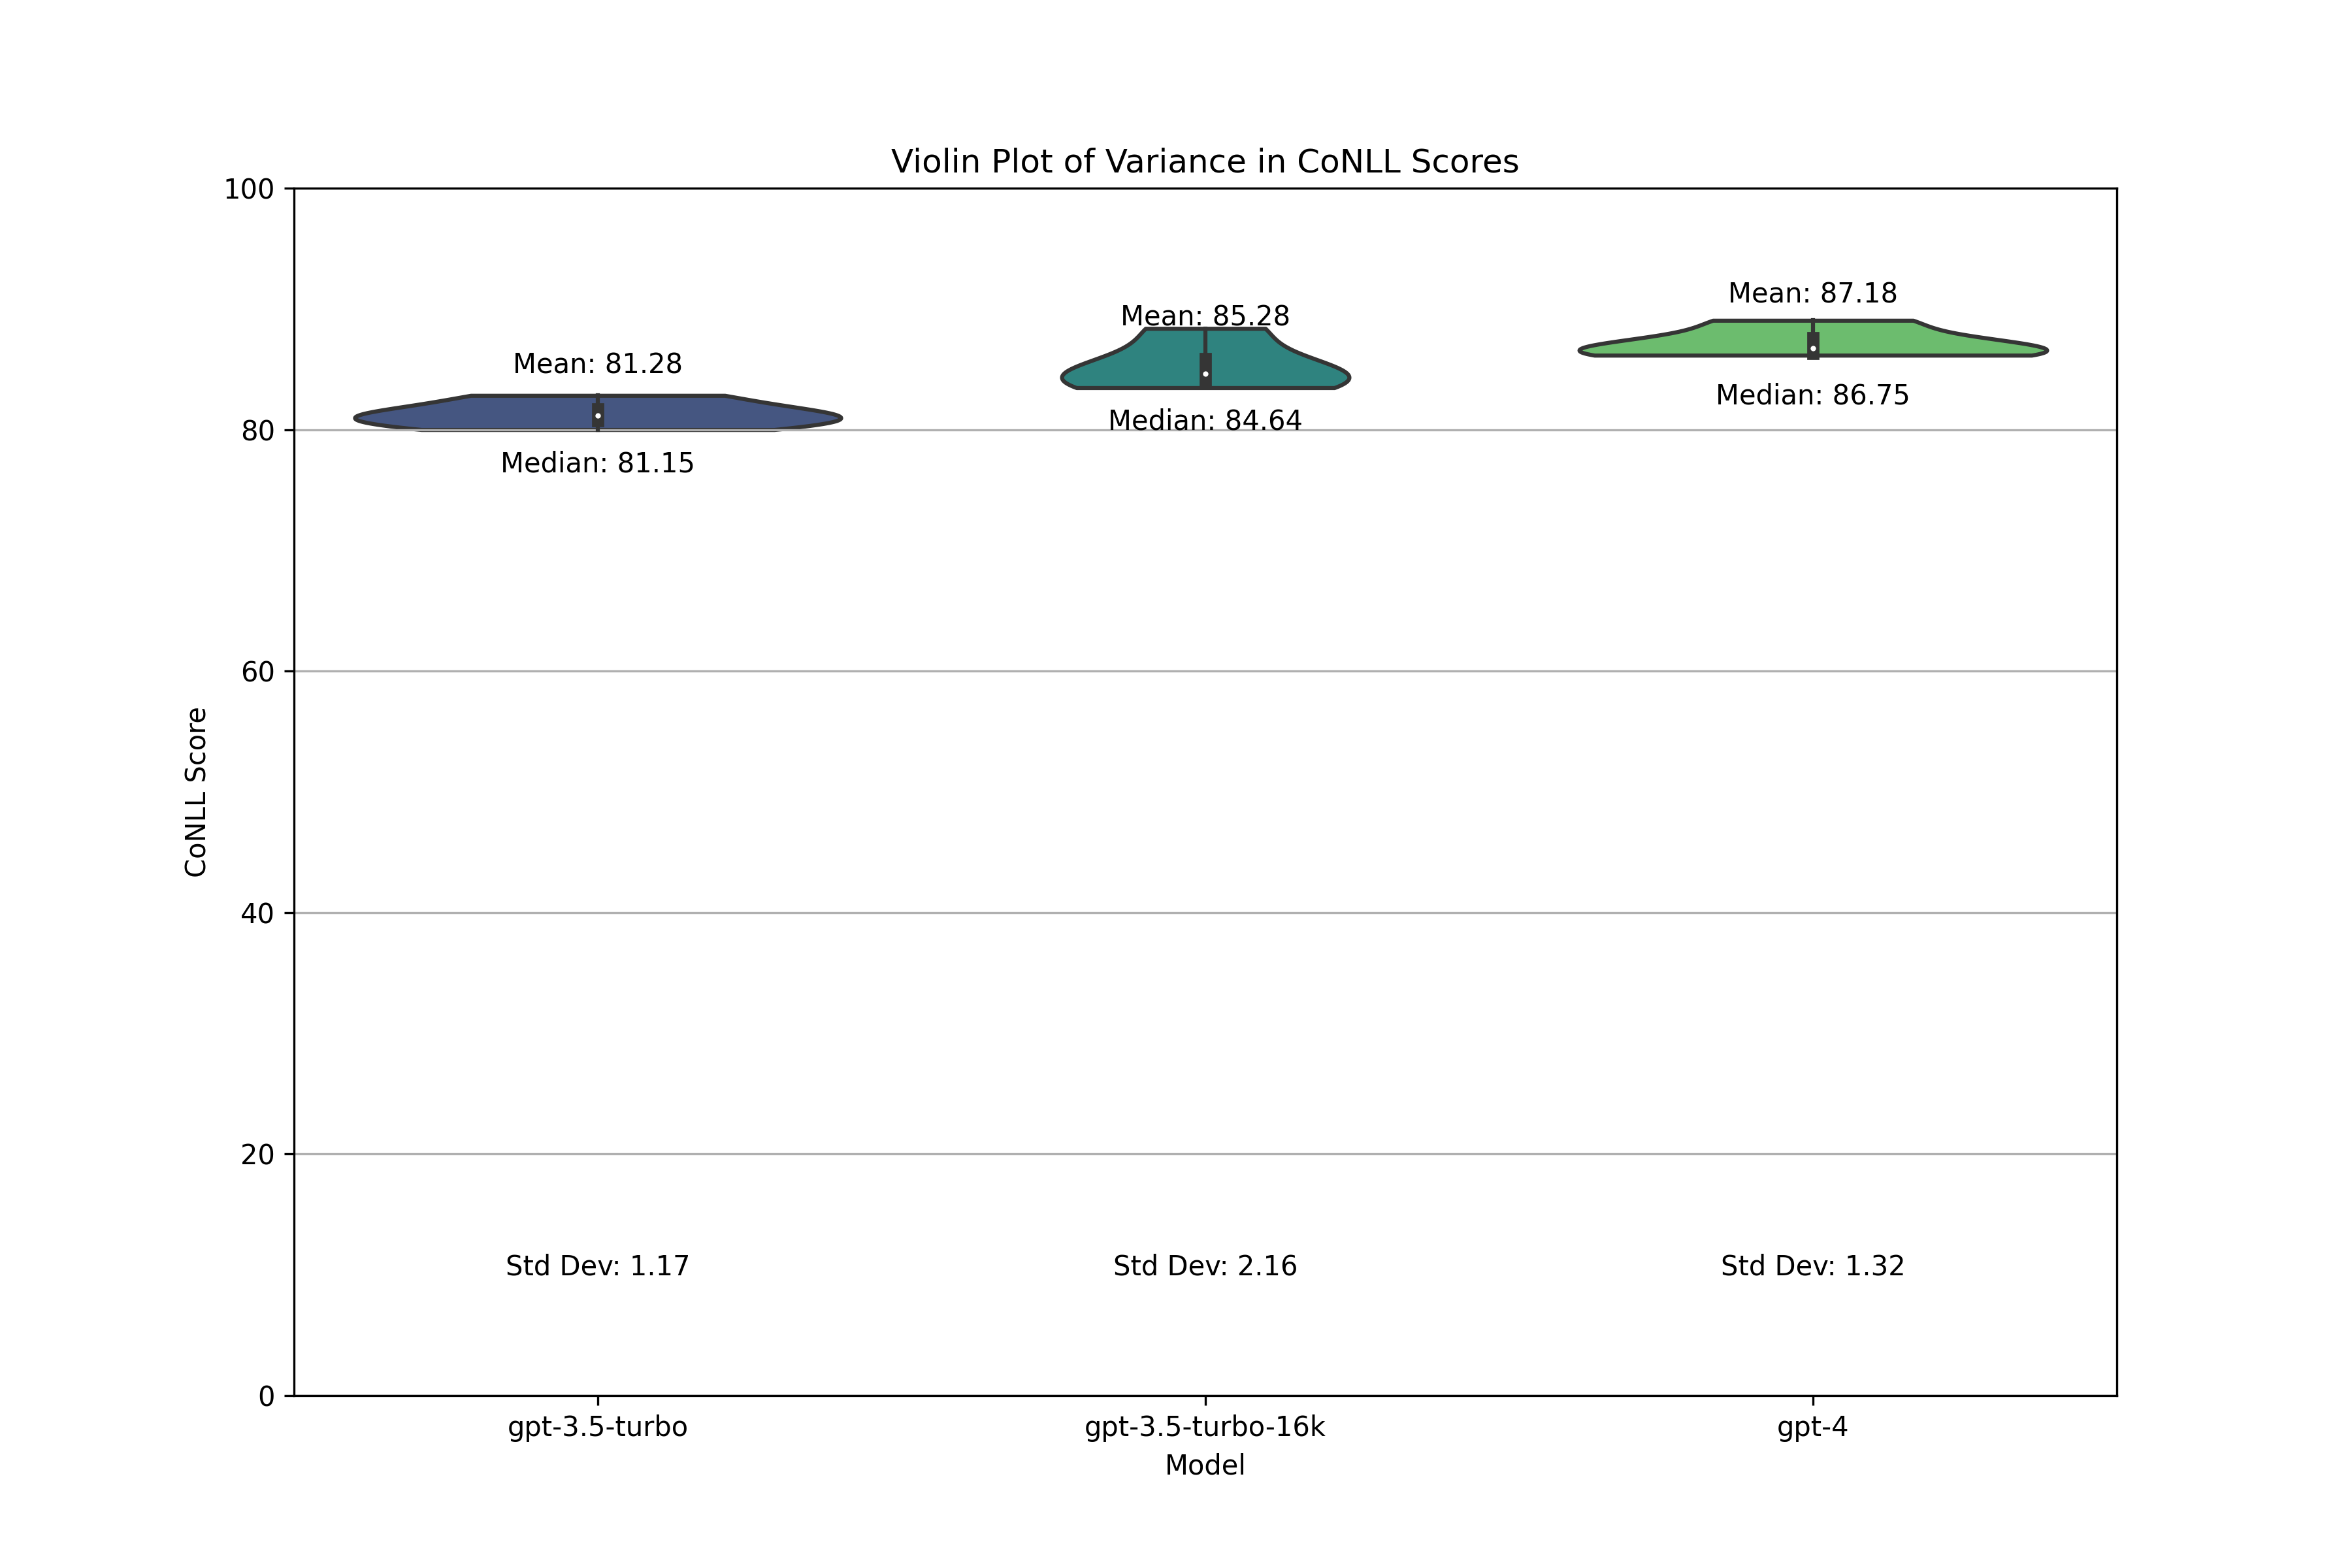
\includegraphics[width=14cm]{images/variance-conll.png}
  \end{tabular}
  \caption[The variance]{Violin Plot of the CoNLL scores for same paper four times}\label{fig:violin-variance}
\end{figure}

\subsection{Running Time and Costs}

The financial aspects of utilising GPT models are quantified through token usage. A comprehensive visualisation of the average costs and time durations for our experiments is provided in Figure \ref{fig:gpt-cost-anal}. It is crucial to note that the length of the paper influences both these metrics under consideration. To offer a more standardised comparison, we present the costs normalised per 1,000 annotations in Figure \ref{fig:gpt-relative-cost}.

Another pivotal dimension is the trade-off between cost and time efficiency. While the ideal scenario would be to minimise both, practical constraints often make this challenging. This relationship is further explored in Figure \ref{fig:gpt-time-v-cost}.

GPT-3.5 emerged as the most cost-effective and time-efficient option among the models evaluated. This efficiency is attributable to OpenAI's competitive token pricing and additional optimisations. Conversely, GPT-4 incurred the highest expenses due to its elevated token costs. GPT-3.5 and GPT-4 demonstrated remarkable stability, contributing to their lower time expenditures. On the other hand, GPT-3.5-16k exhibited instability, leading to increased time costs.

\begin{figure}[htpb]
  \centering
  \subfloat[Average Cost of Annotation]{
    \begin{tabular}{c}
  \hspace*{-.25cm}
  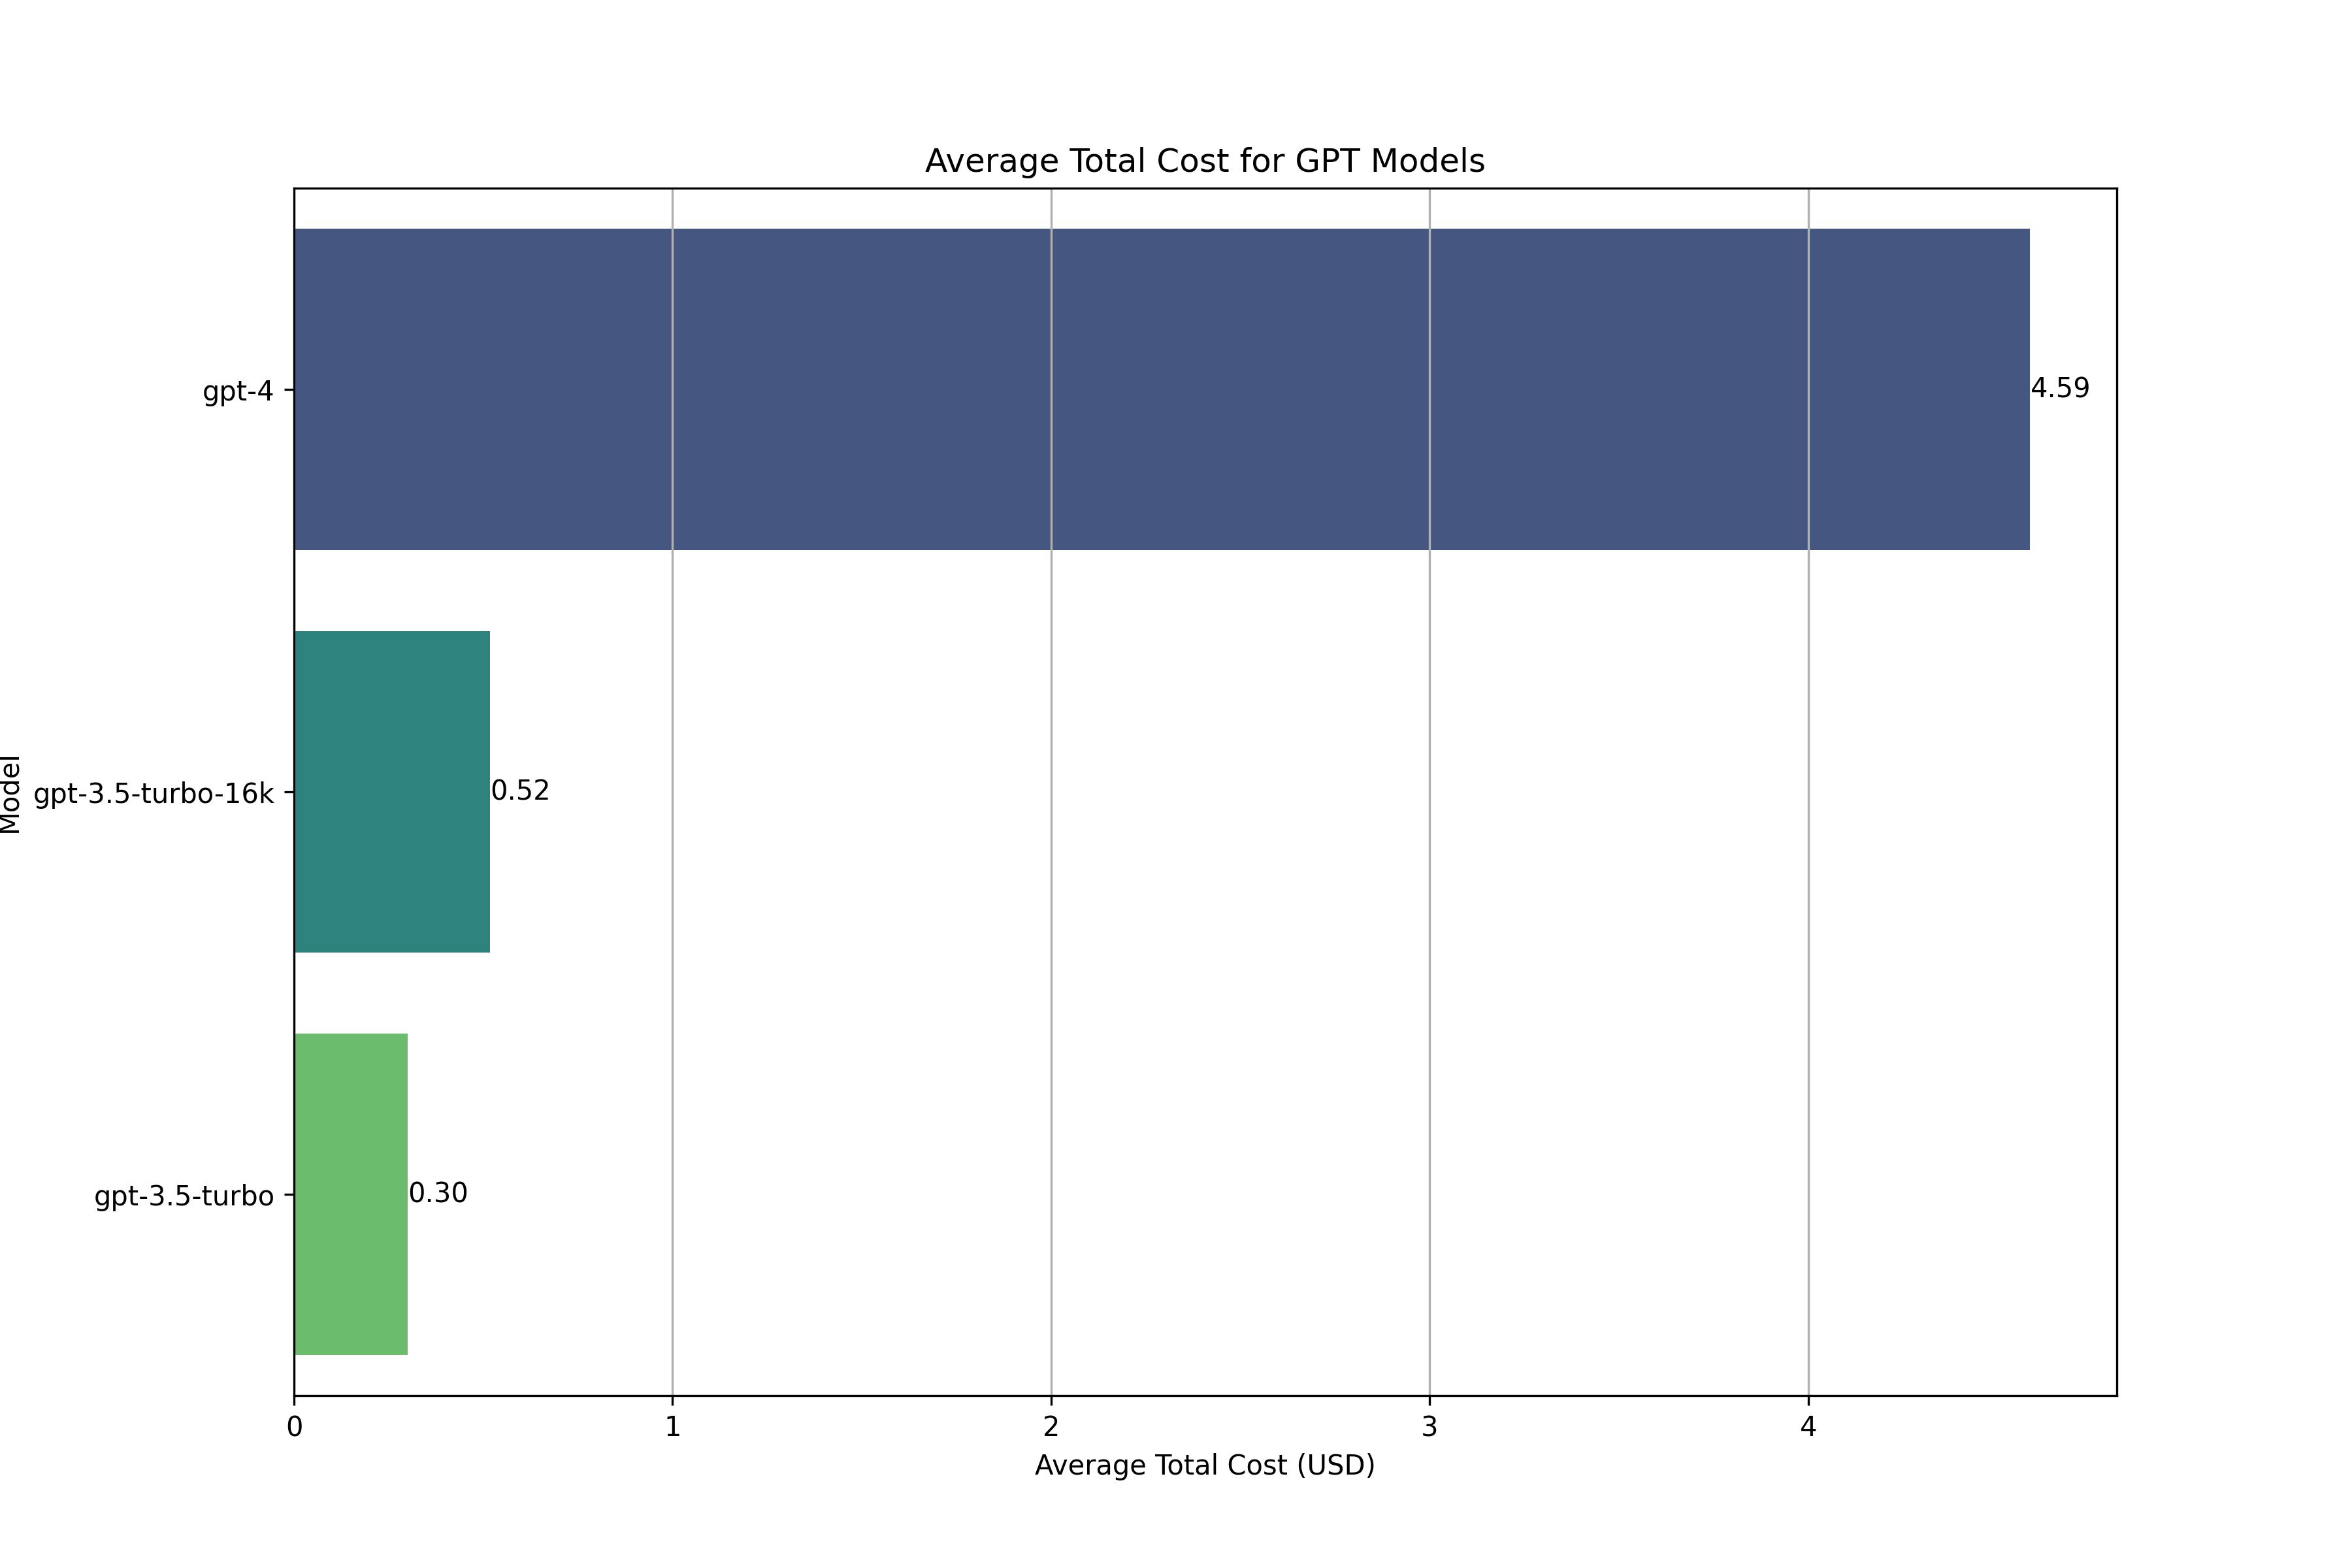
\includegraphics[width=11cm]{images/cost-gpt.png}
  \end{tabular}
  }
  \quad 
  \subfloat[Average Duration of Annotation]{
    \begin{tabular}{c}
  \hspace*{-1.5cm}
  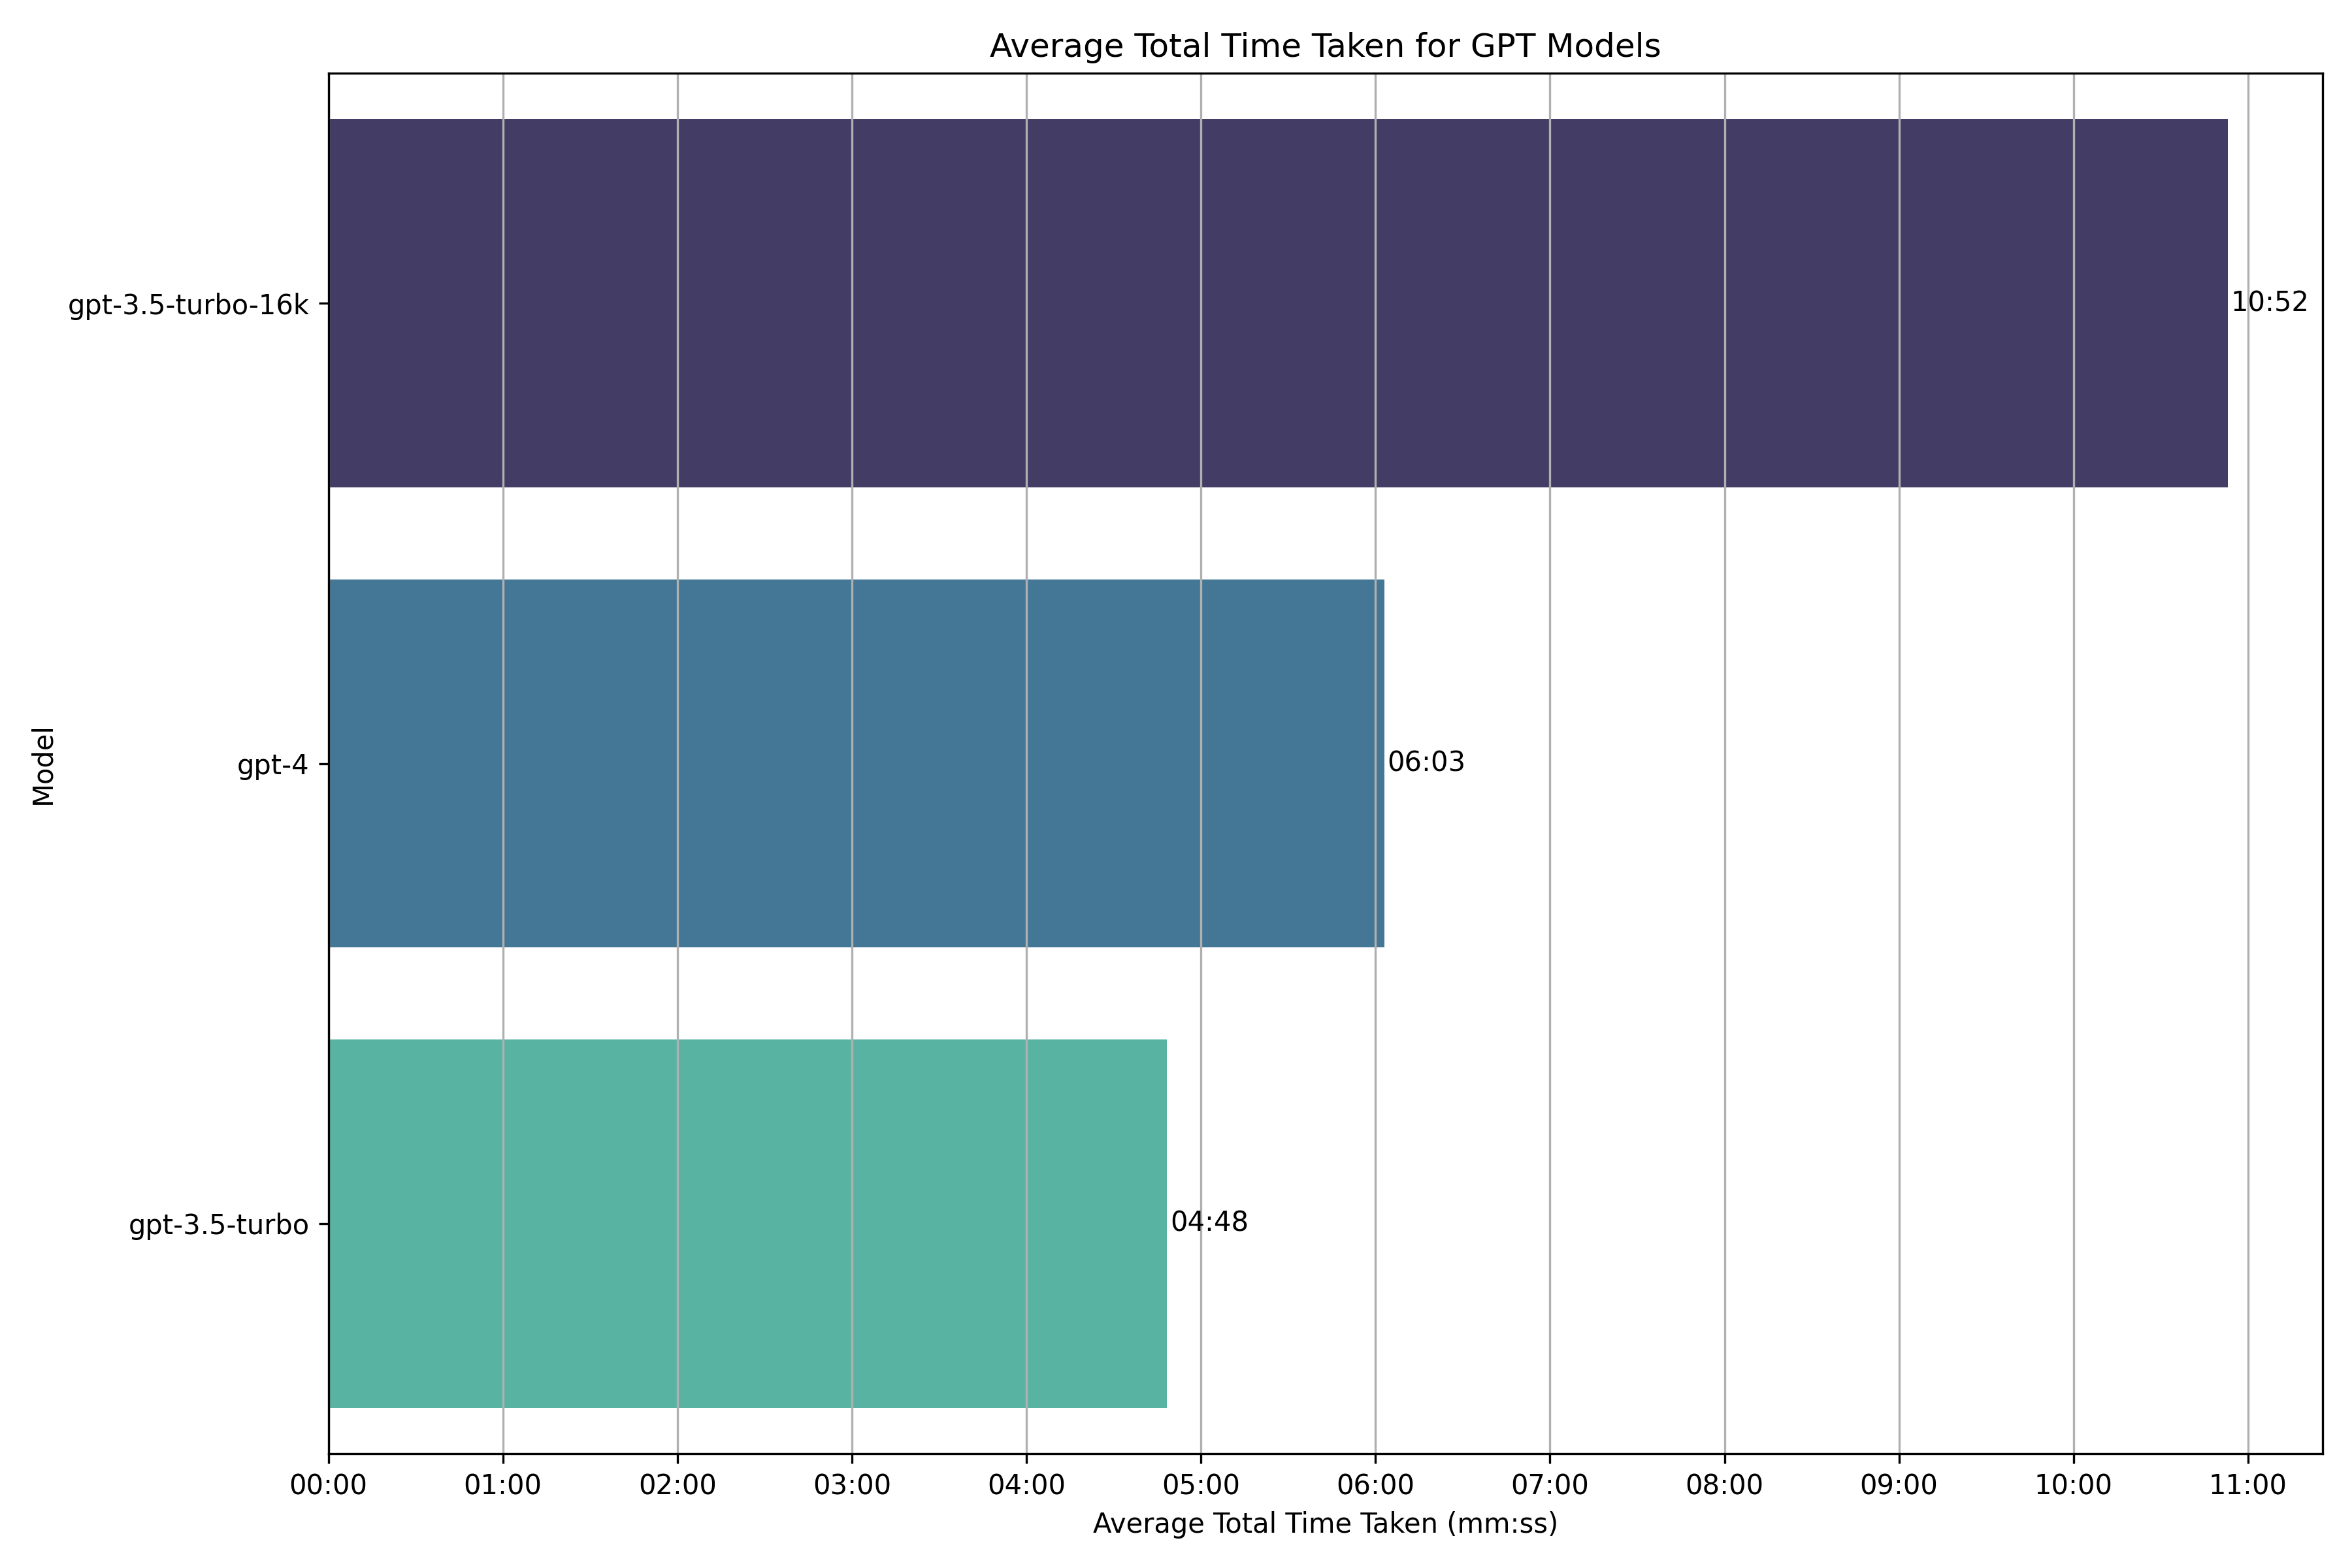
\includegraphics[width=10cm]{images/time-gpt.png}
  \end{tabular}
  }
  \caption[Cost Analysis]{Cost and Time Usage of Annotations}\label{fig:gpt-cost-anal}
\end{figure}

\begin{figure}[htpb]
  \centering
  \subfloat[Average Cost per 1000 Concept]{
    \begin{tabular}{c}
  %\hspace*{-.25cm}
  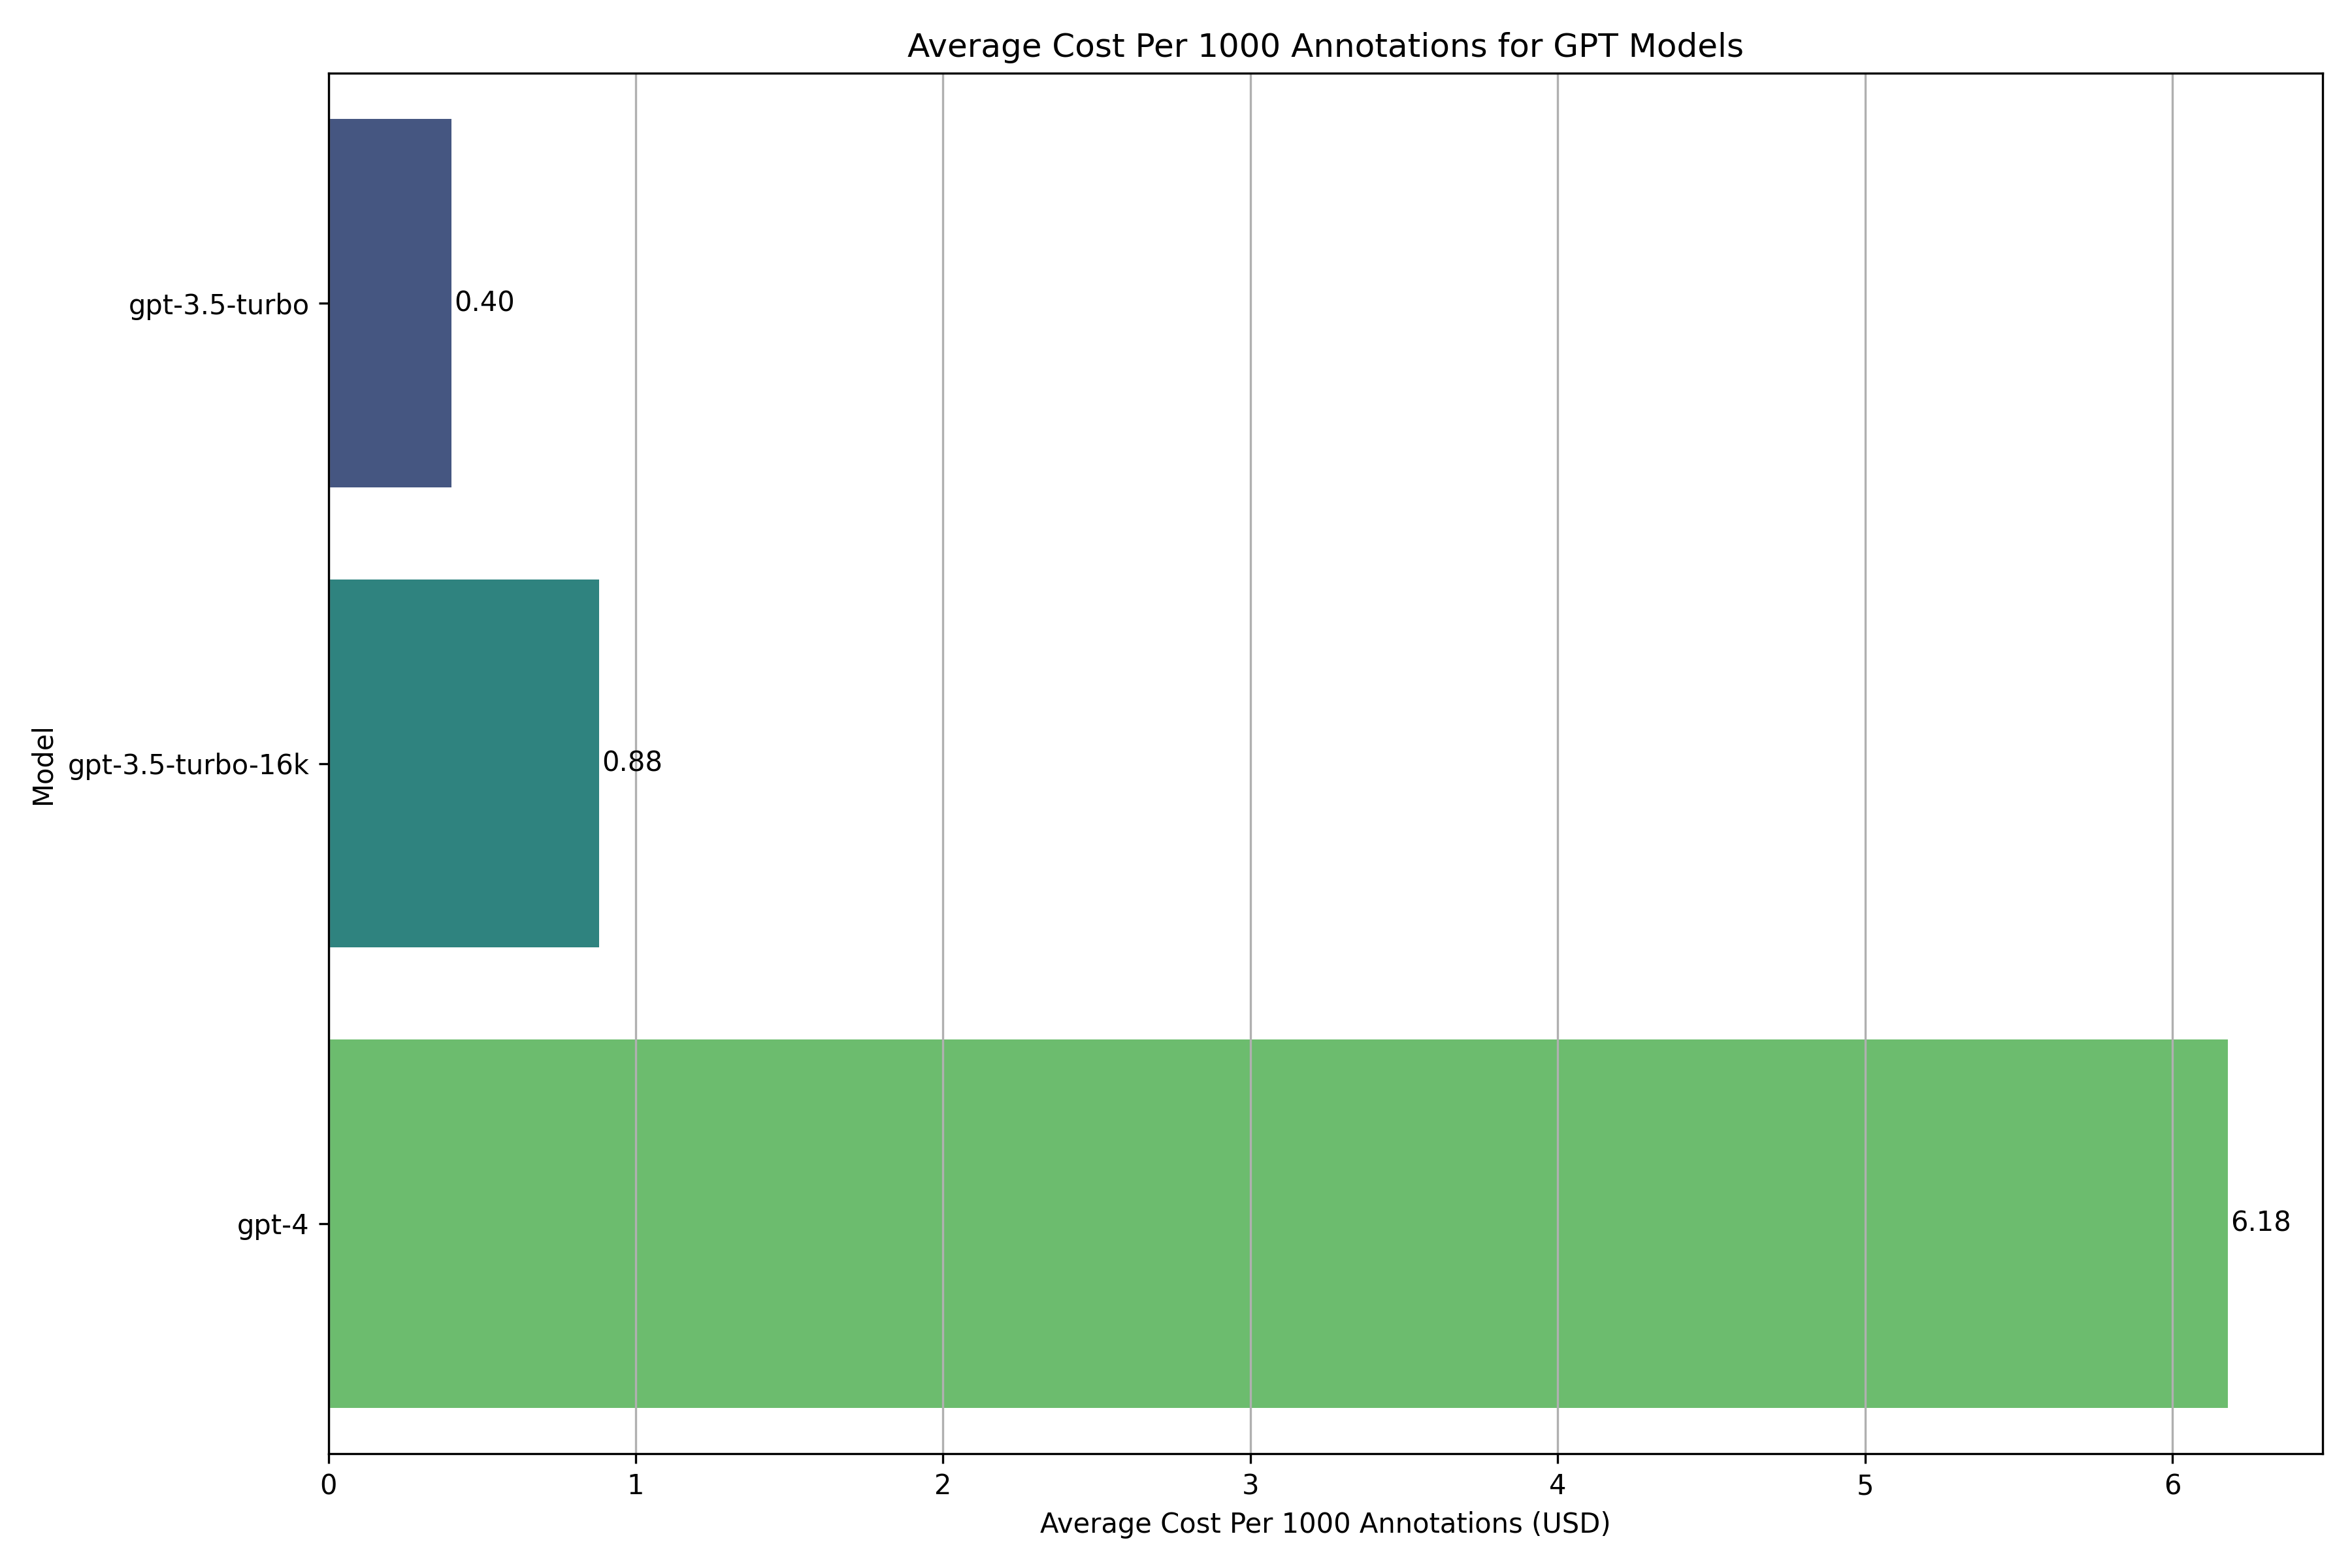
\includegraphics[width=11cm]{images/gpt-relative-cost.png}
  \end{tabular}
  }
  \quad 
  \subfloat[Average Duration per Concept]{
    \begin{tabular}{c}
  %\hspace*{-1.5cm}
  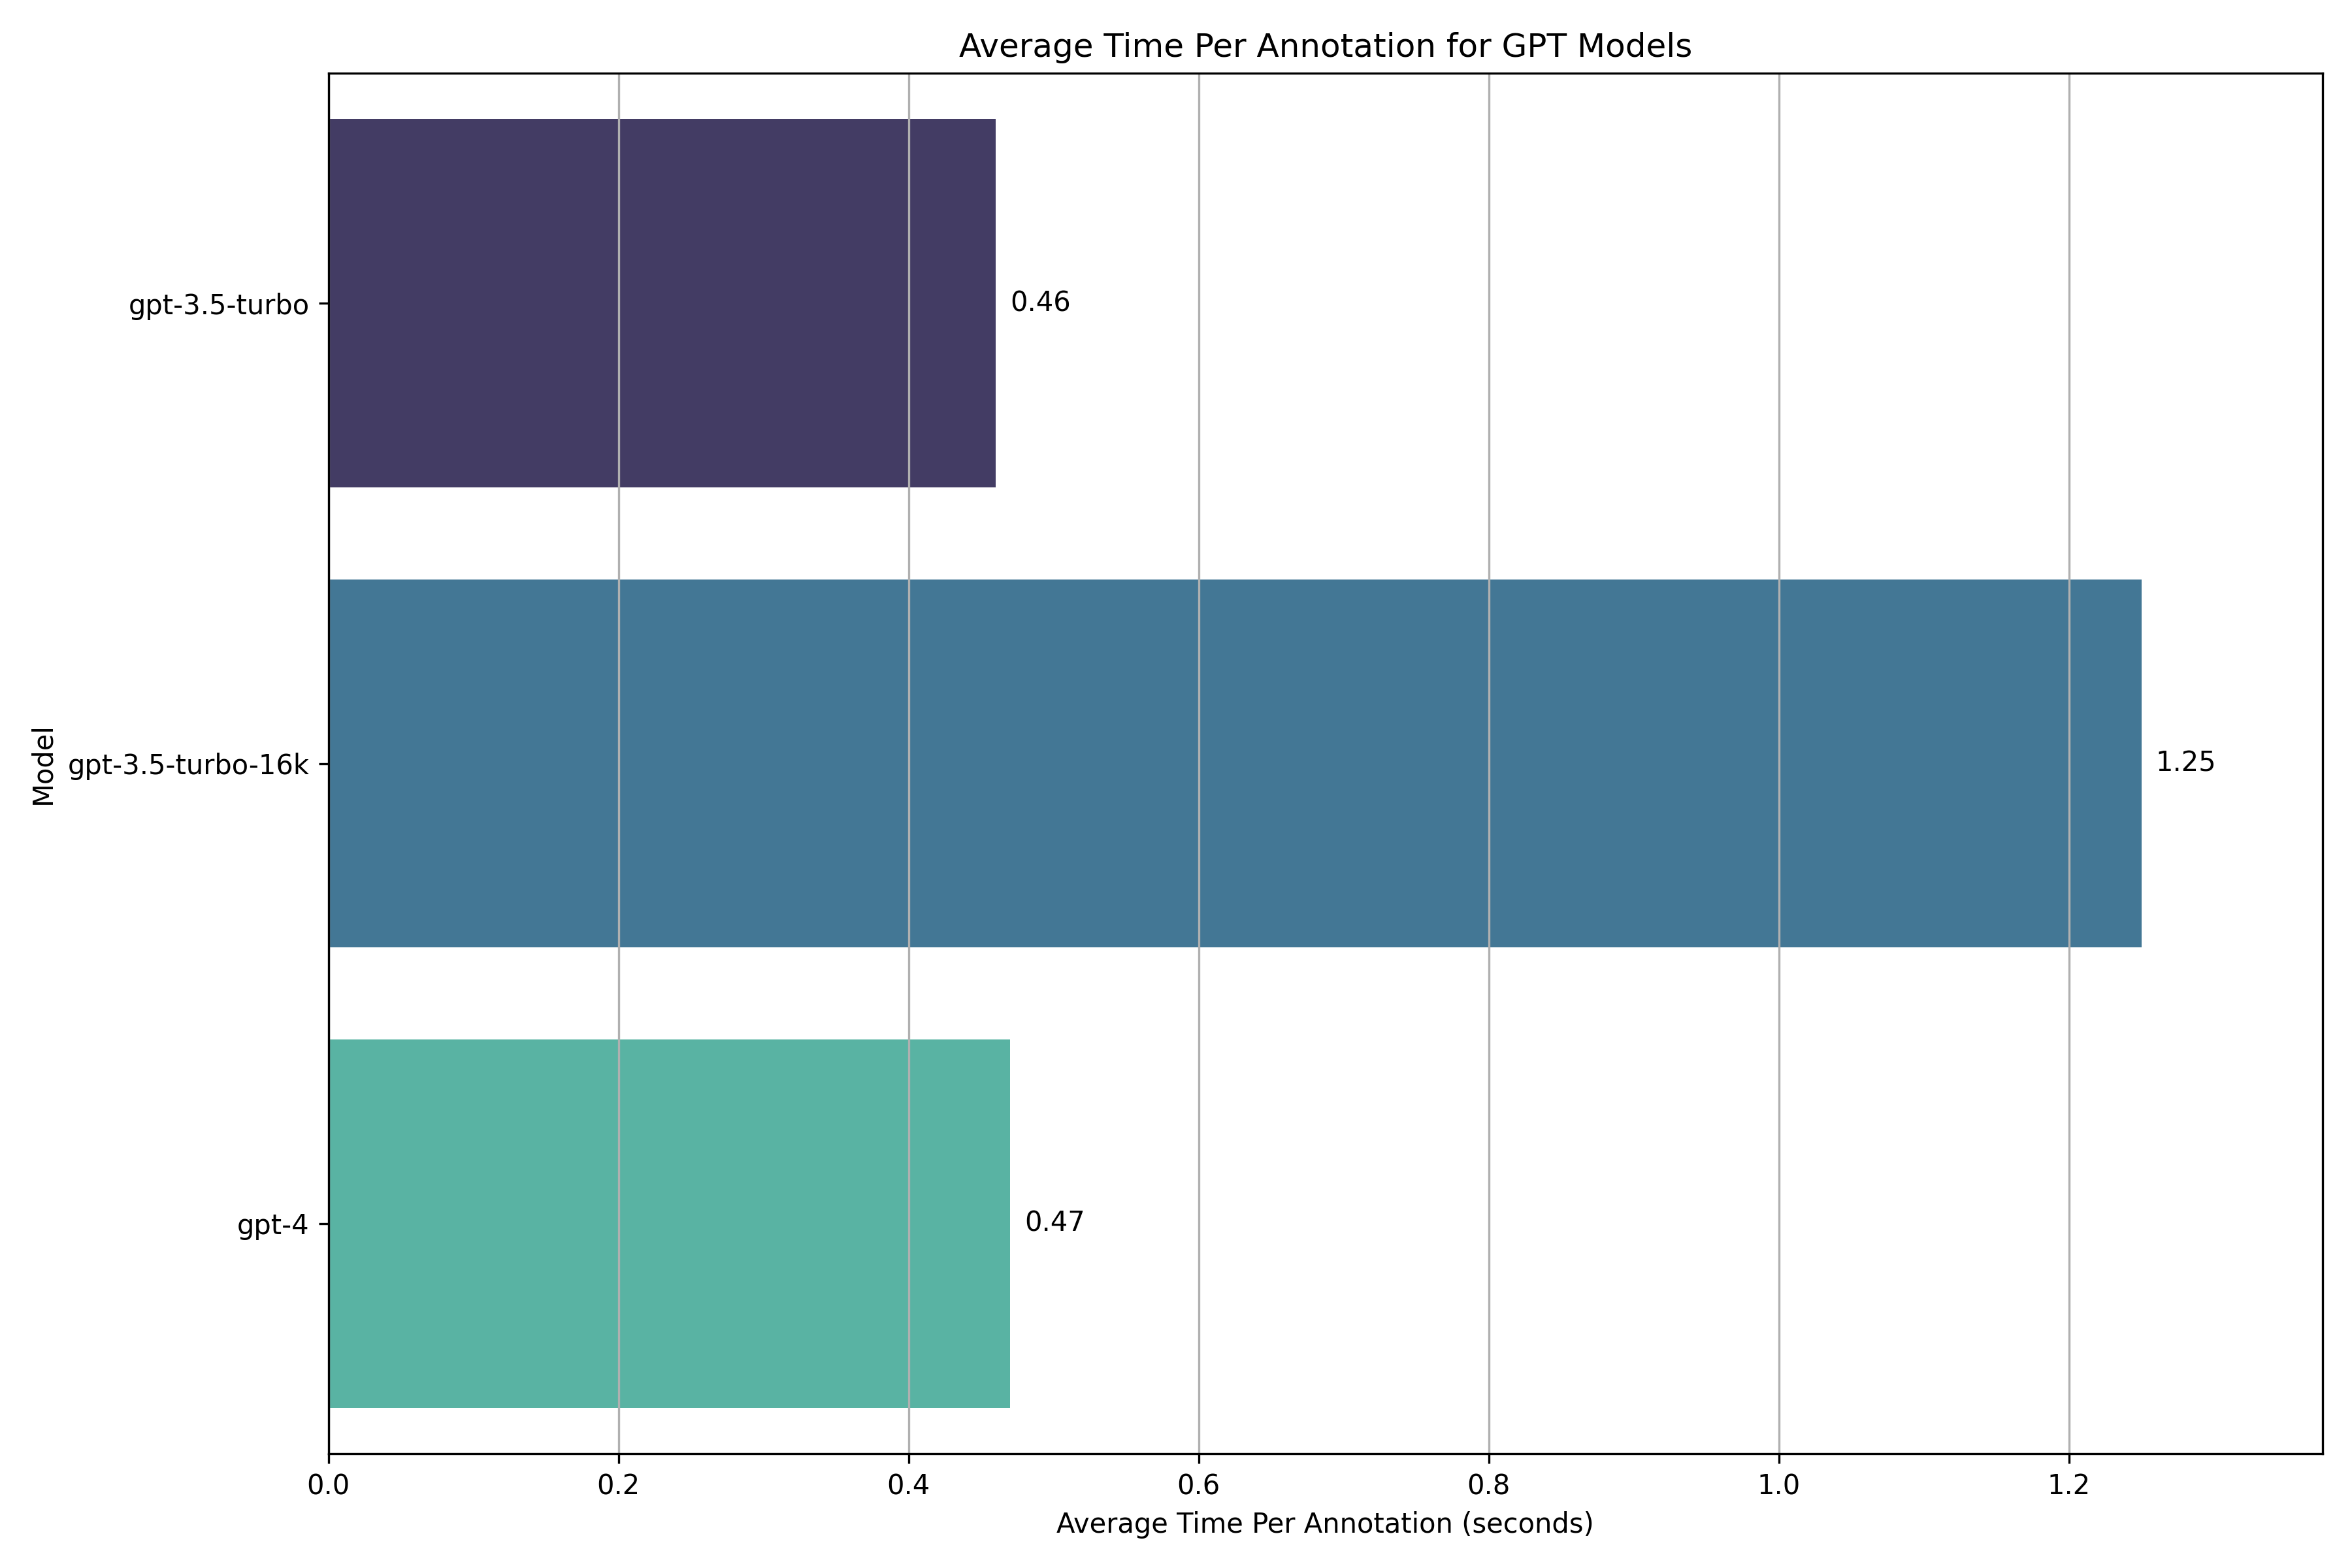
\includegraphics[width=10cm]{images/gpt-relative-time.png}
  \end{tabular}
  }
  \caption[Time Cost Analysis]{Cost and Time Usage of Automation}\label{fig:gpt-relative-cost}
\end{figure}

\begin{figure}[htpb]
  \centering
  \begin{tabular}{c}
  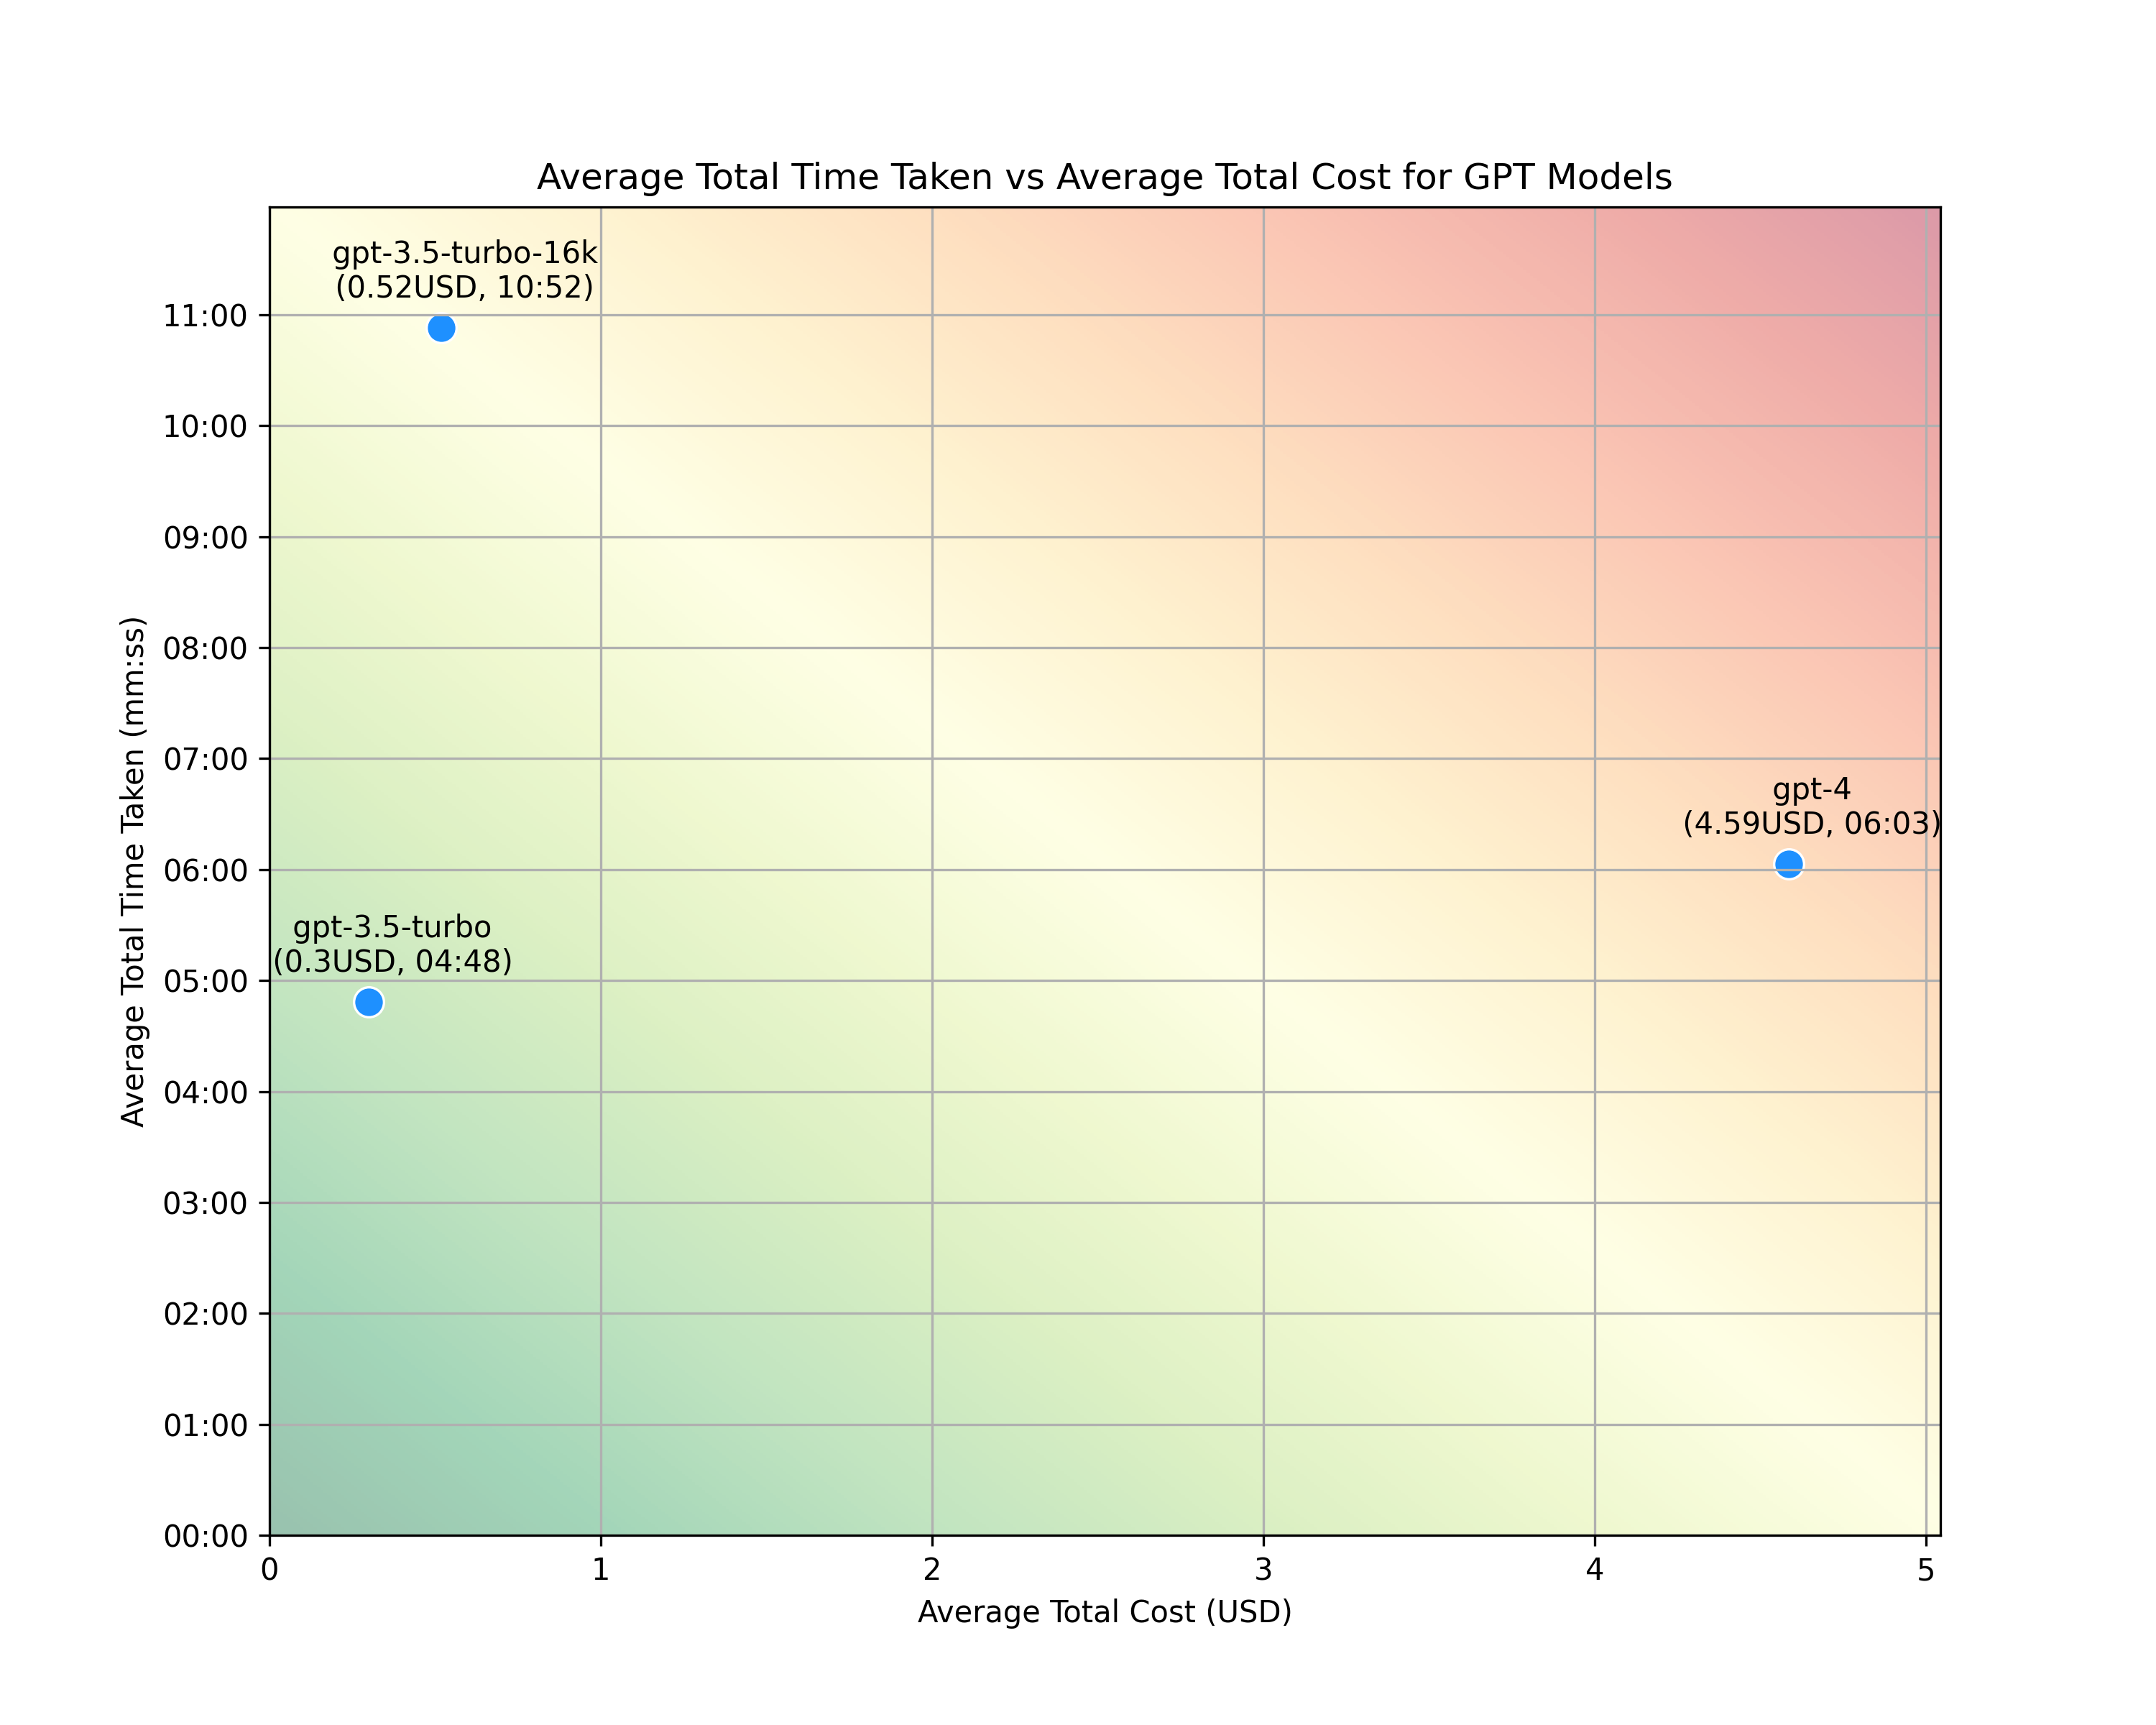
\includegraphics[width=14cm]{images/gpt-time-v-cost.png}
  \end{tabular}
  \caption[Cost vs Time]{Scatter Plot of Average Cost vs Time Taken}\label{fig:gpt-time-v-cost}
\end{figure}


\section{Open Souce LLMs}

We then scrutinised the annotations generated by OpenSource Models. We used a smaller subset of 7 papers from the 40 generated by \citet{asakura2022building} as the ground truth for this analysis. Then, we employed it to generate dictionaries and annotations for all these papers. The Open Source models varied in terms of their performance drastically. Among the two models we evaluated, Vicuna-33b lagged noticeably behind GPT models in performance. This outcome is expected because Vicuna-33b operates on a 33-billion parameter architecture. However, it is noteworthy that a scale model still demonstrates a formula grounding capability.

Conversely, StableBeluga2 exhibited remarkable performance, nearly matching that of GPT-4. This is particularly impressive, considering StableBeluga2 operates on a 70-billion parameter framework, while GPT-4 is rumoured to have a staggering 1.8 trillion parameters. Moreover, StableBeluga2 consistently outperformed GPT-3.5 across multiple metrics. This superior performance is likely attributable to the specialised nature of StableBeluga2, designed as an "instruct" model, in contrast to GPT models that are general-purpose chat models not explicitly optimised for formula grounding.

\subsection{CoNLL Score}

Vicuna-33b struggled in several cases, even scoring zero in one instance, hinting at its inability to generate any meaningful dictionary for that paper. StableBeluga2, on the other hand, aptly managed to deliver performances that stood almost on par with GPT Models as illustrated in Figure \ref{fig:open-source-conll}. Despite this, GPT models maintained a discernible edge in disambiguation capabilities over their open-source counterparts. This advantage is likely attributable to the extensive training that GPT models undergo.

\begin{figure}[htpb]
  \centering
  \begin{tabular}{c}
  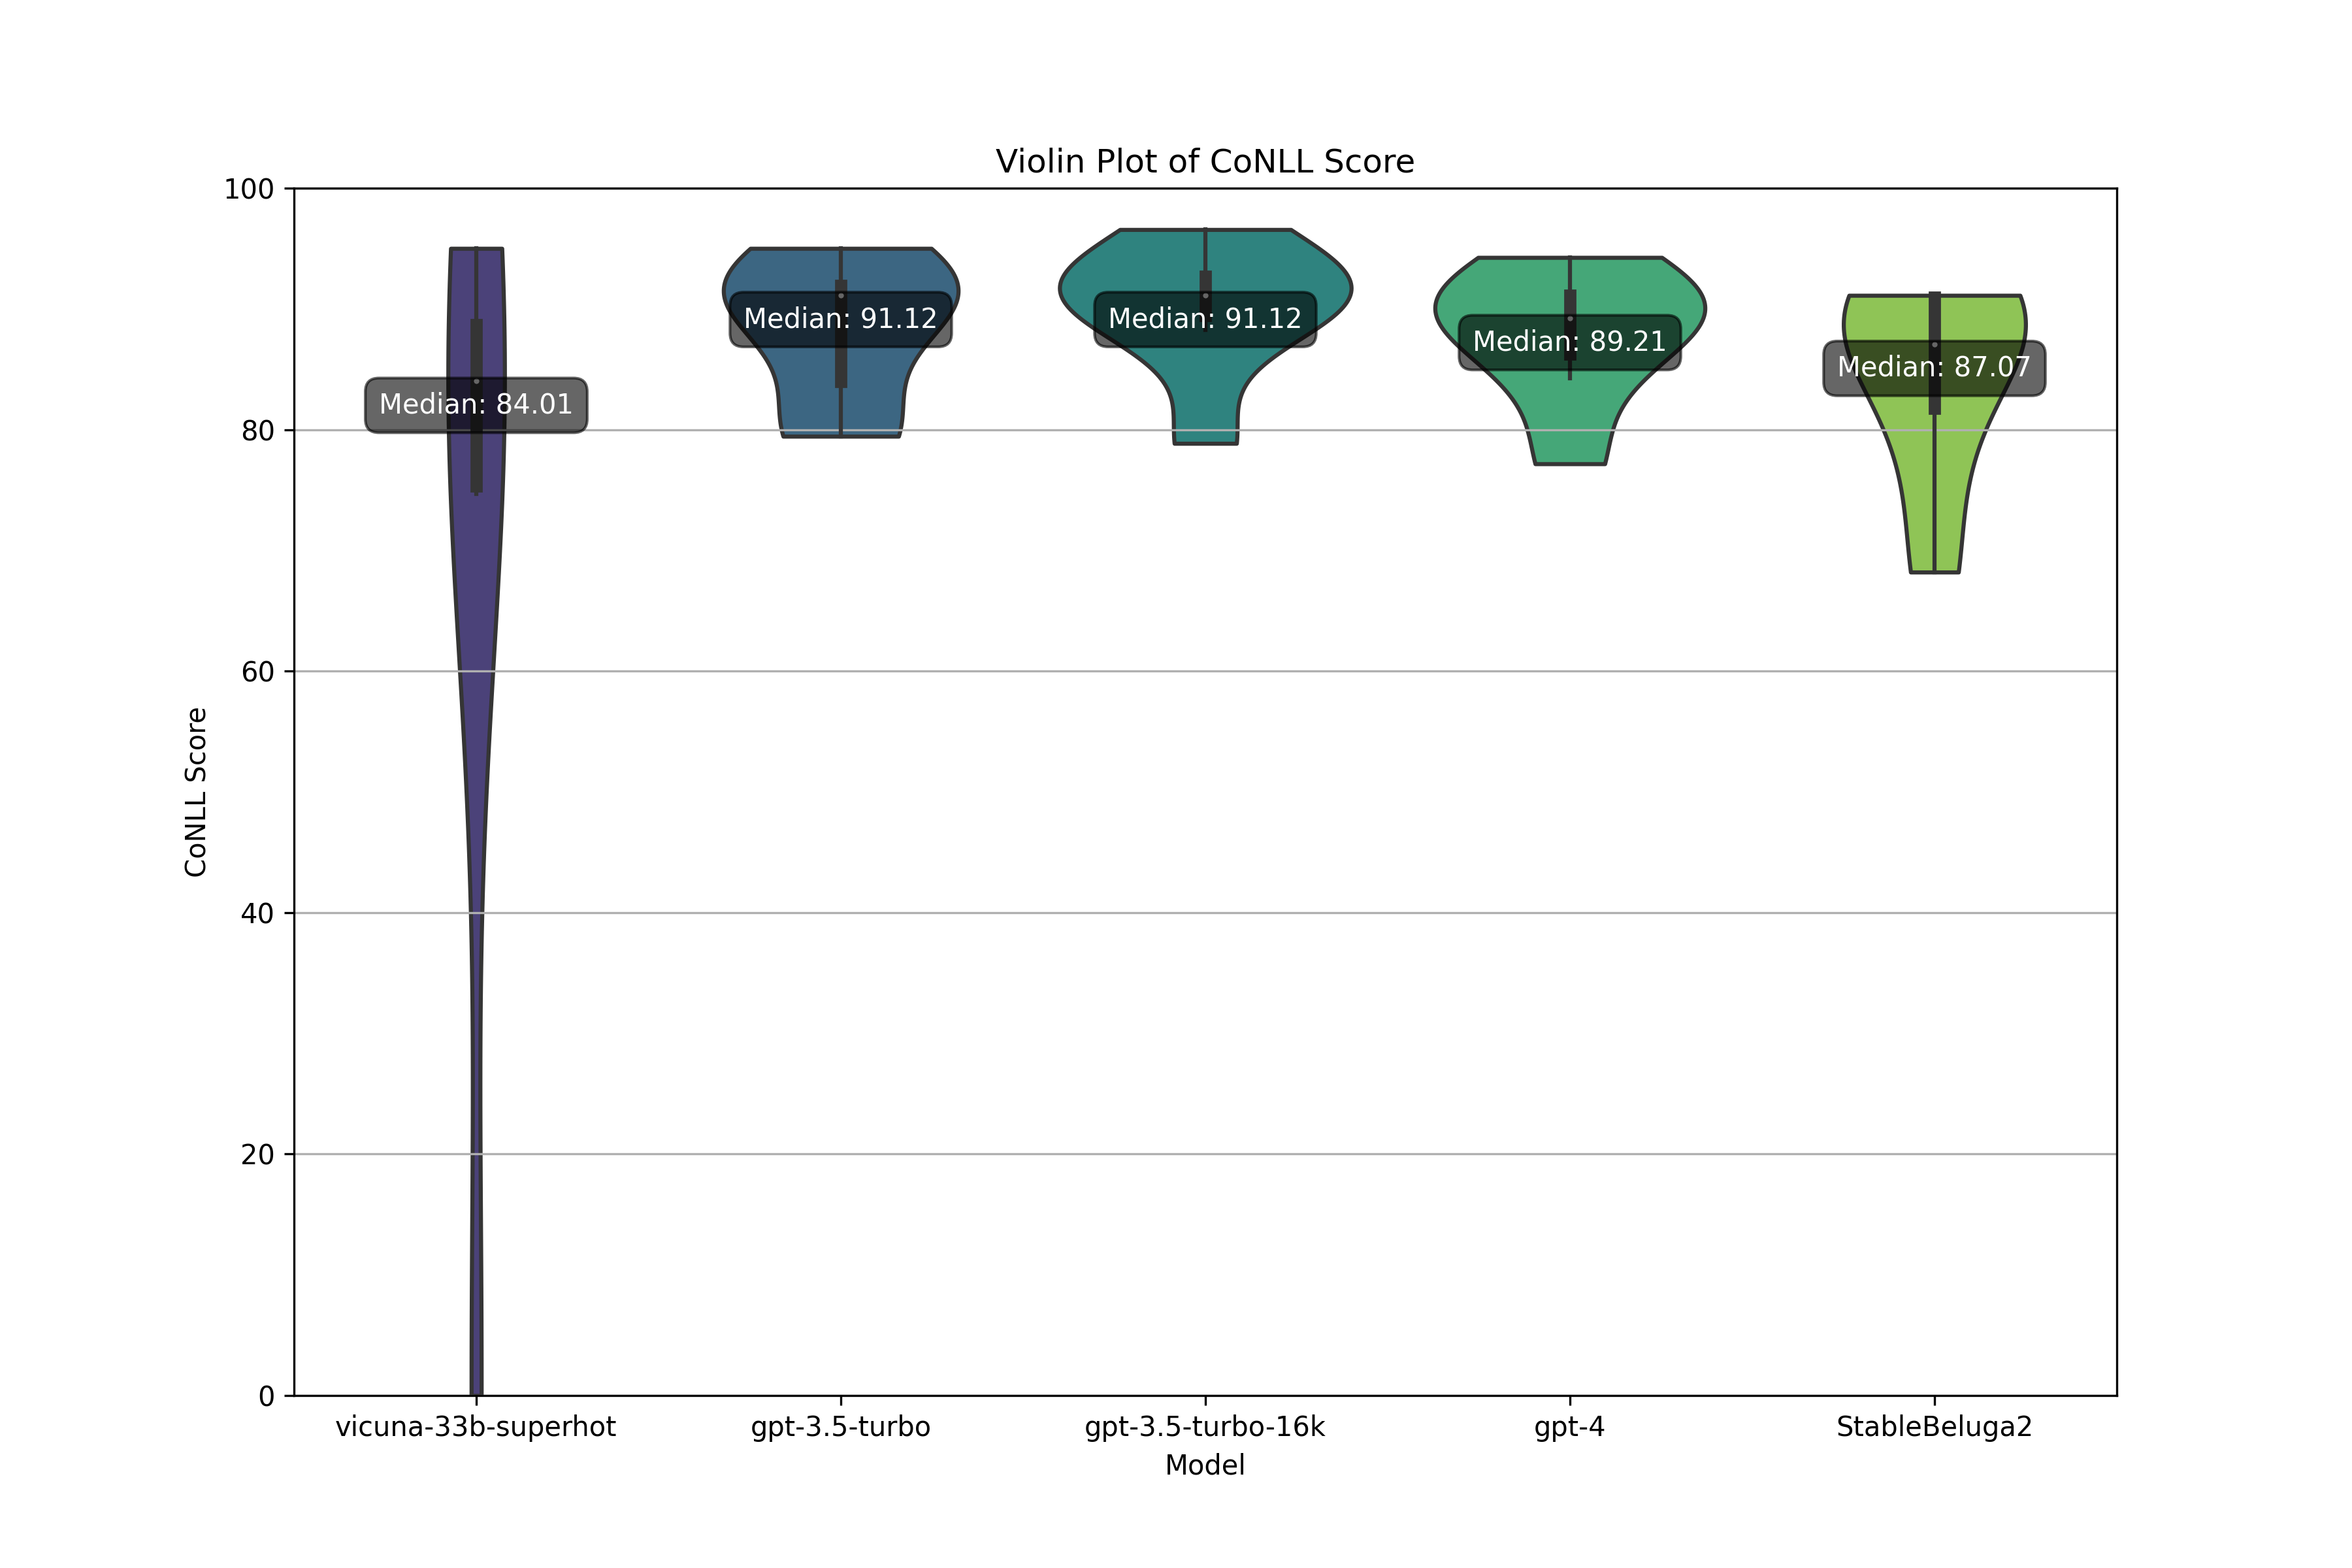
\includegraphics[width=14cm]{images/open-conll-score.png}
  \end{tabular}
  \caption[CoNLL Score Open Source]{Violin Plot of the CoNLL scores using all 5 models}\label{fig:open-source-conll}
\end{figure}

\subsection{Coverage of Annotation}

Once again, vicuna-33b faced challenges in providing complete coverage for one paper, resulting in a score of zero. StableBeluga2, achieving performances comparable to GPT Models, presents an insightful contrast as further evidenced in Figure \ref{fig:open-coverage}. Despite this isolated setback for Vicuna-33b, its performance generally remains subpar compared to its more advanced counterparts. 

\begin{figure}[htpb]
  \centering
  \begin{tabular}{c}
  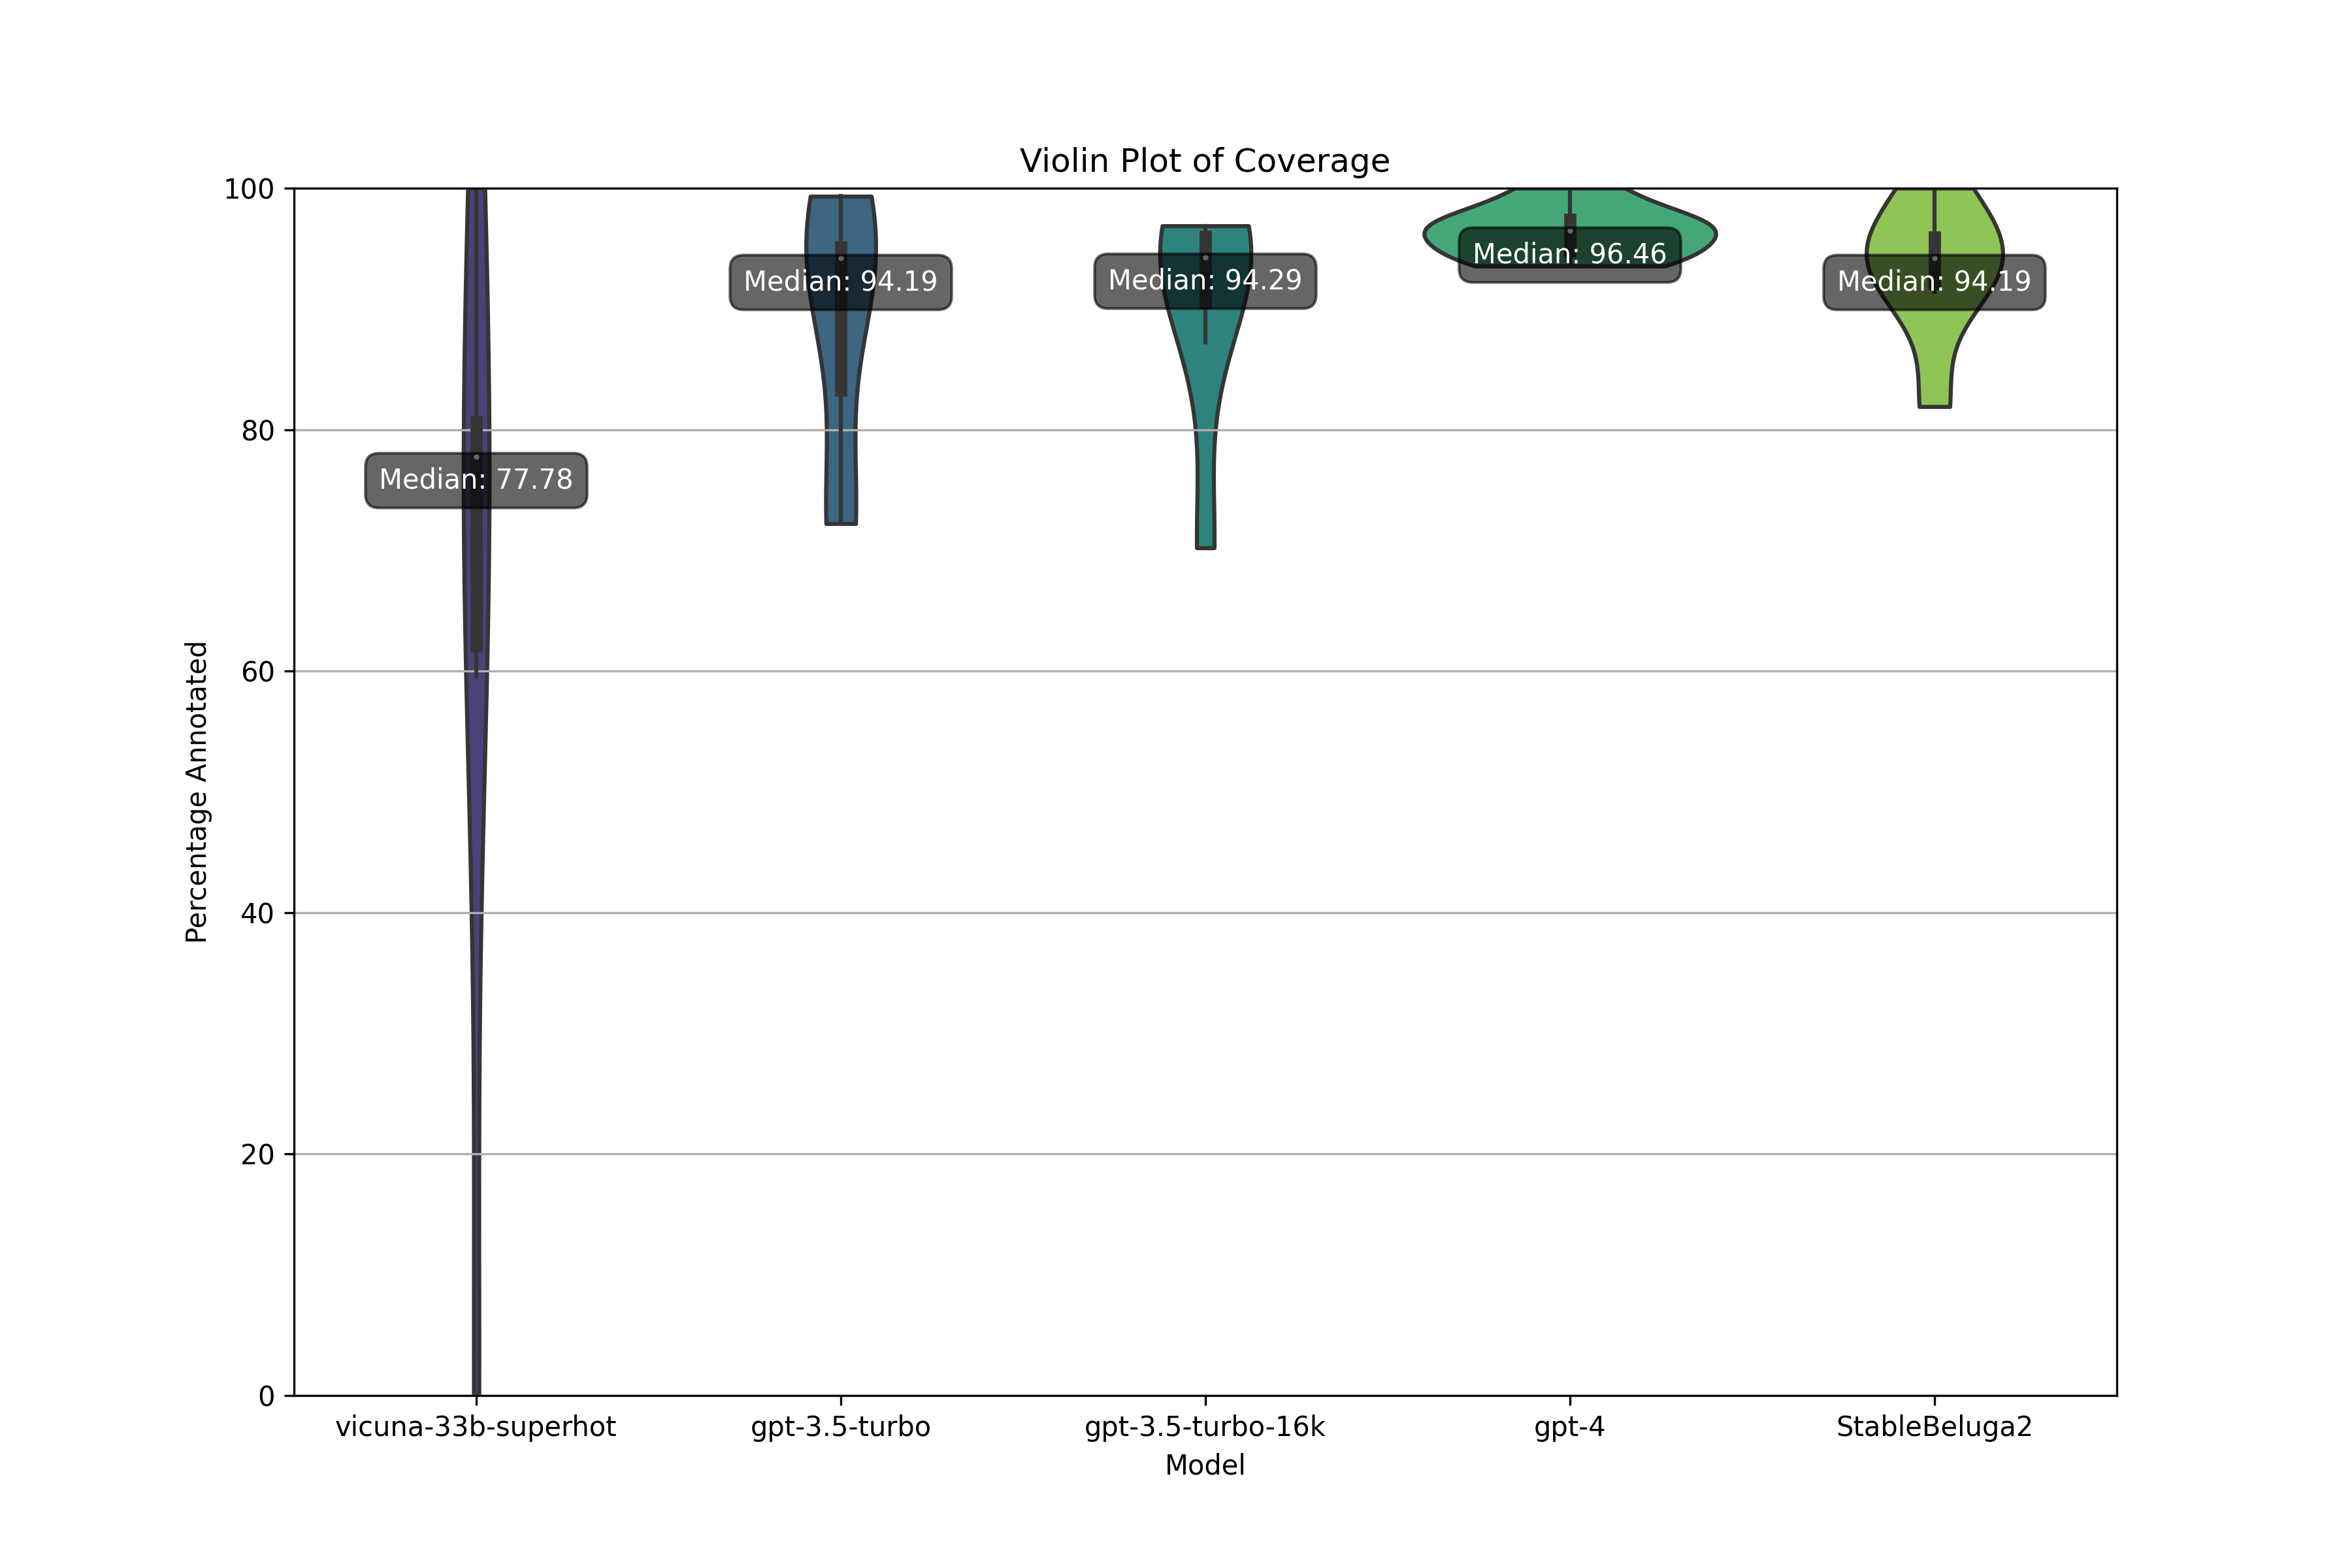
\includegraphics[width=14cm]{images/open-coverage.png}
  \end{tabular}
  \caption[Open Source Coverage]{Violin Plot of the coverage of the papers annotated}\label{fig:open-coverage}
\end{figure}

\subsection{Semantic Accuracy}

Semantic accuracy functions as the cornerstone of our comparative study. Due to the labour-intensive nature of manual evaluation, we selected a subset of six papers for this purpose. StableBeluga2, an Open Source LLM, beats GPT-3.5 entirely yet could not surpass GPT-4, which deserves mention due to the unmatched complexity and sophistication of GPT-4's architecture. As detailed in Figure \ref{fig:open-semantic}, the semblance between the performance of StableBeluga2 and GPT models reinforces this open-source model's potential in accurately understanding and reflecting the context of scientific papers. Vicuna-33b's performance was notably lacklustre, a limitation likely attributable to its smaller model size.

\begin{figure}[htpb]
  \centering
  \begin{tabular}{c}
  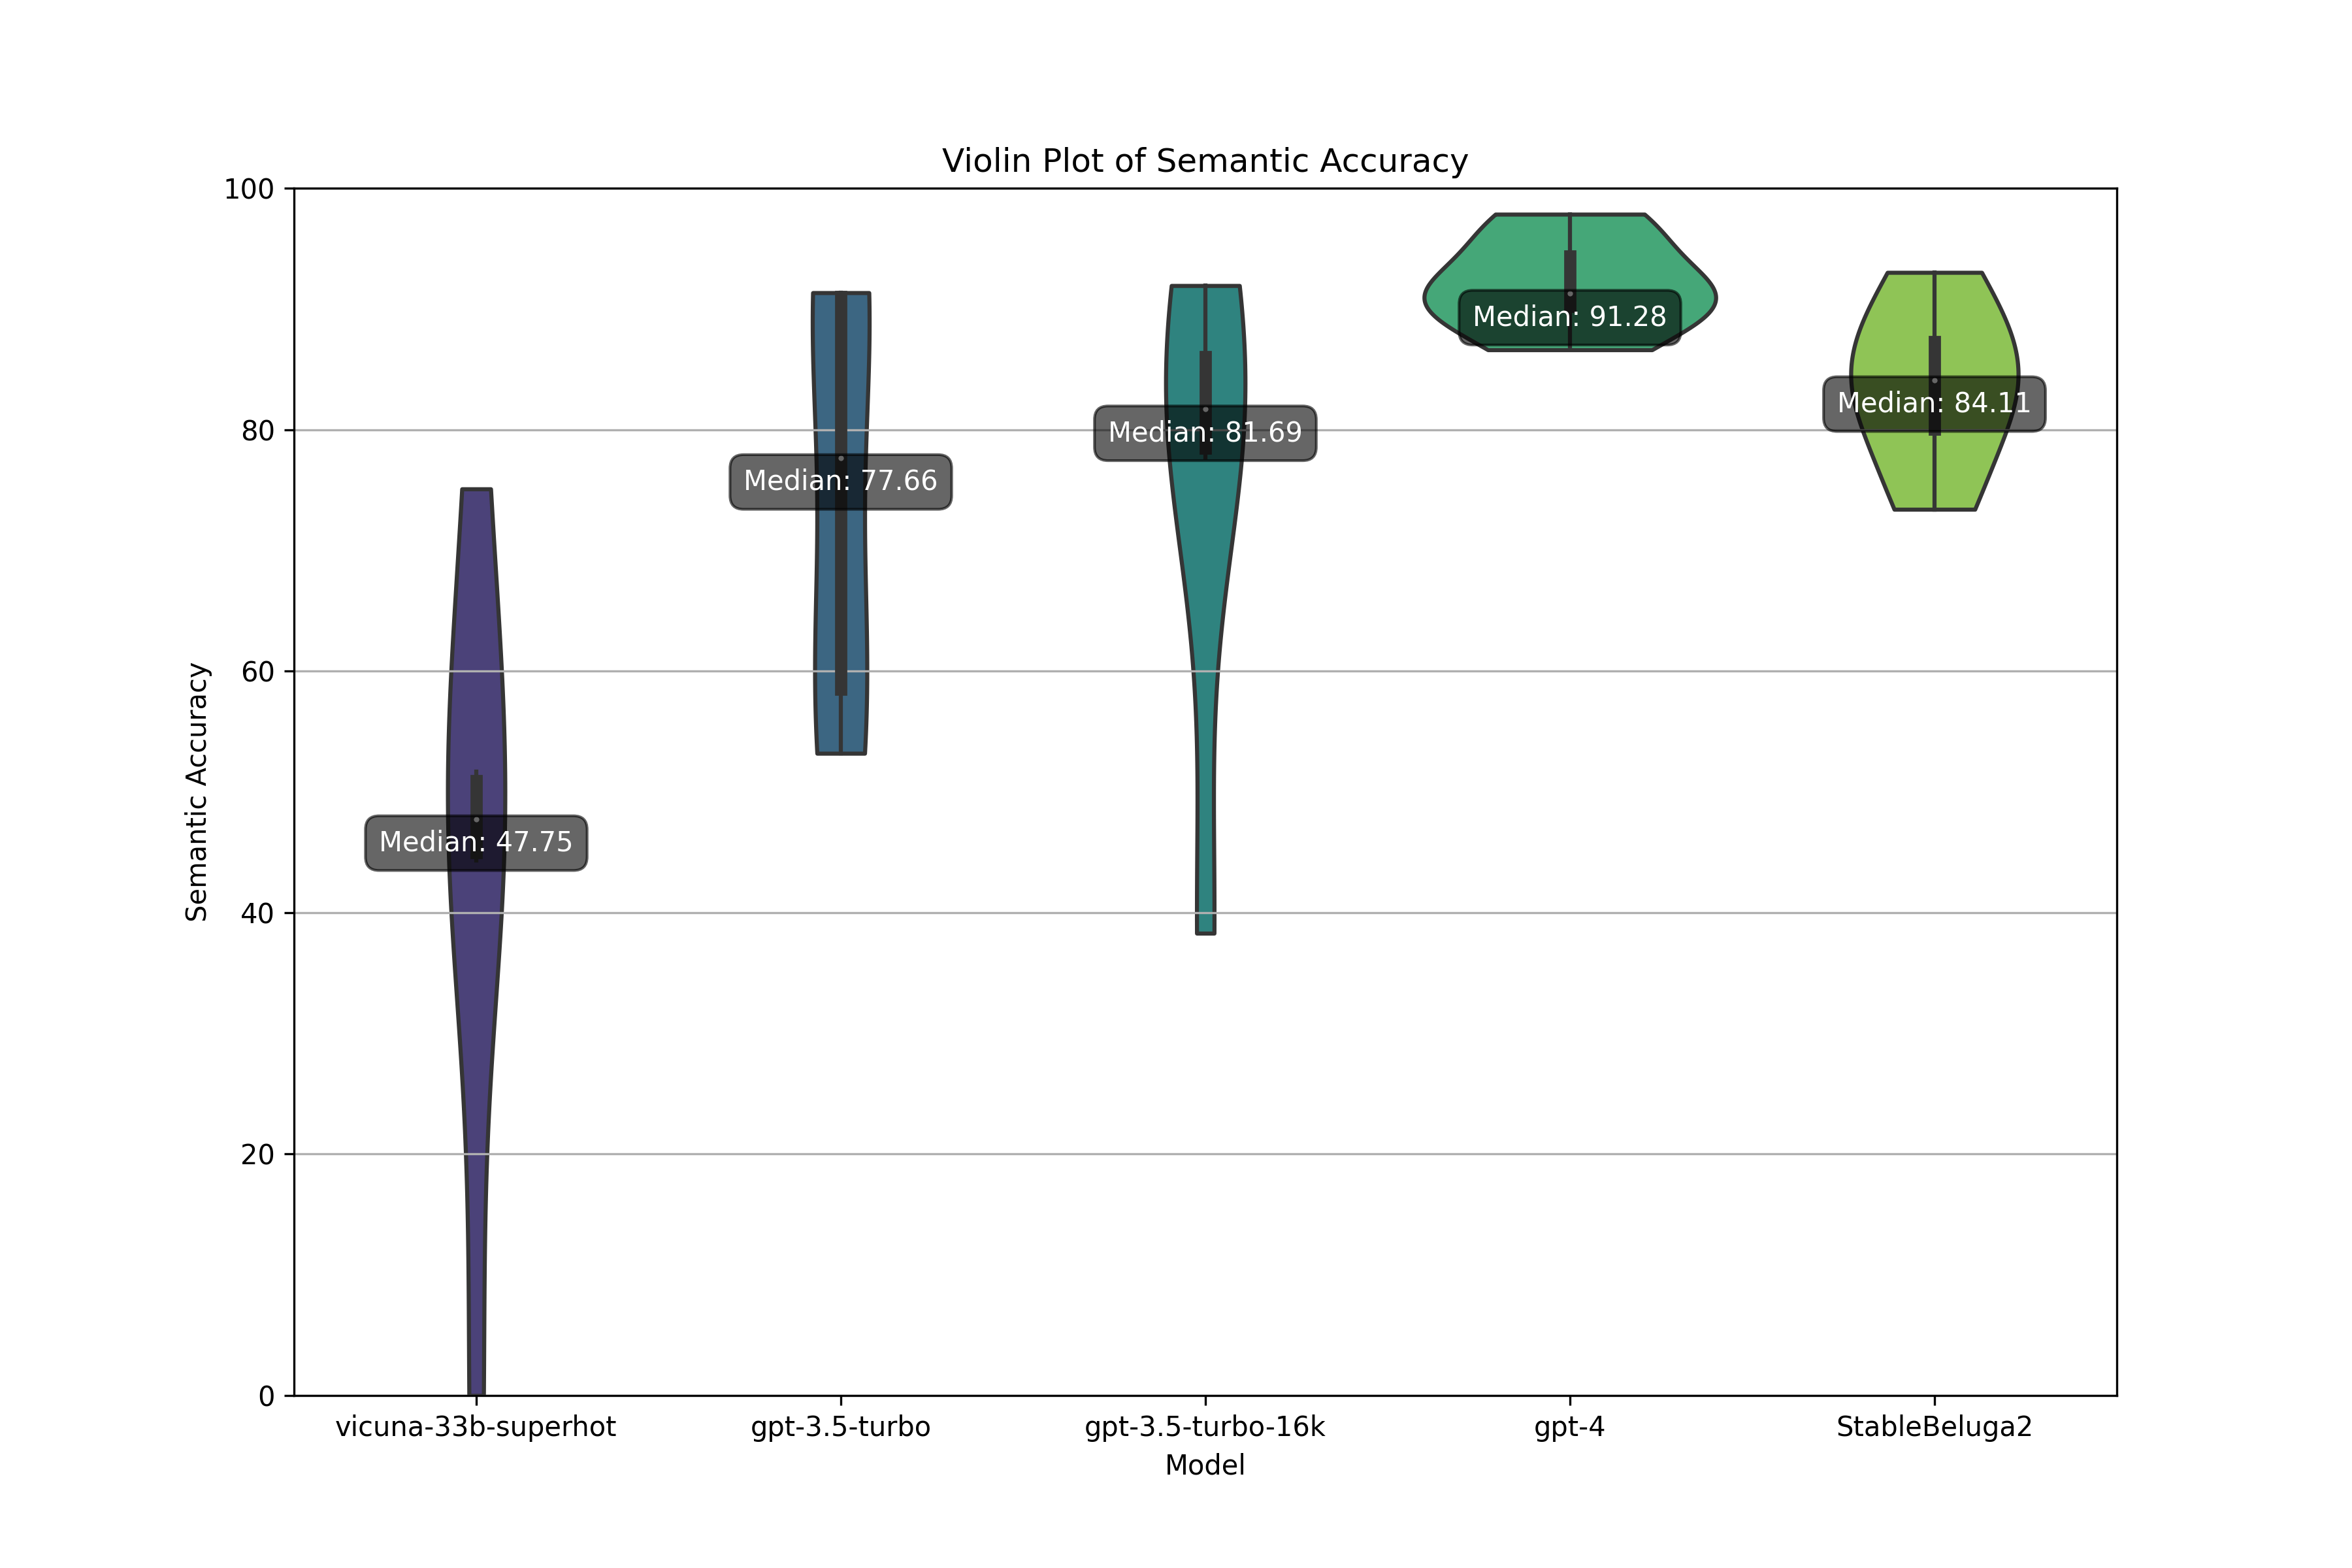
\includegraphics[width=14cm]{images/open-semantic.png}
  \end{tabular}
  \caption[Semantic Accuracy]{Semantic Accuracy Scores from all the 5 models}\label{fig:open-semantic}
\end{figure}

\subsection{Running Time and Costs}

Given the distinctive operational requirements of open-source models, the computation of time and cost efficiencies differ from those of GPT models. Unlike GPT models, the cost for open-source models revolves around GPU runtime, and in our case, on the servers of \href{https://runpod.io}{runpod.io} and not token usage. The running time is visualised in Figure \ref{fig:open-runtime}. However, since the time taken here depends on the length of the paper, it is essential to compare the costs per annotation. This can be visualised in \ref{fig:open-relative-cost}. Because of cheaper hardware, the average run time of open-source LLMs was prolonged. On average, they were 5-10x slower. This is especially noticeable for StableBeluga2 as it is a Large LLM. The cost for the experiments can differ from person to person, as we had to pay for the GPU usage. If a person owns GPUs, it will be free of cost; however, regardless, we have visualised the cost we paid for annotations in Figure \ref{fig:open-cost}. It can also very well happen that the cost to use these GPUs is way higher than GPT. GPT-4 is significantly more expensive than all other models. vicuna-33b has a similar operating cost to GPT-3.5 but performs way worse. StableBeluga2, which performs better than GPT-3.5, costs 3x more than GPT-3.5 and 3x less than GPT-4.

\begin{figure}[htpb]
  \centering
  \begin{tabular}{c}
  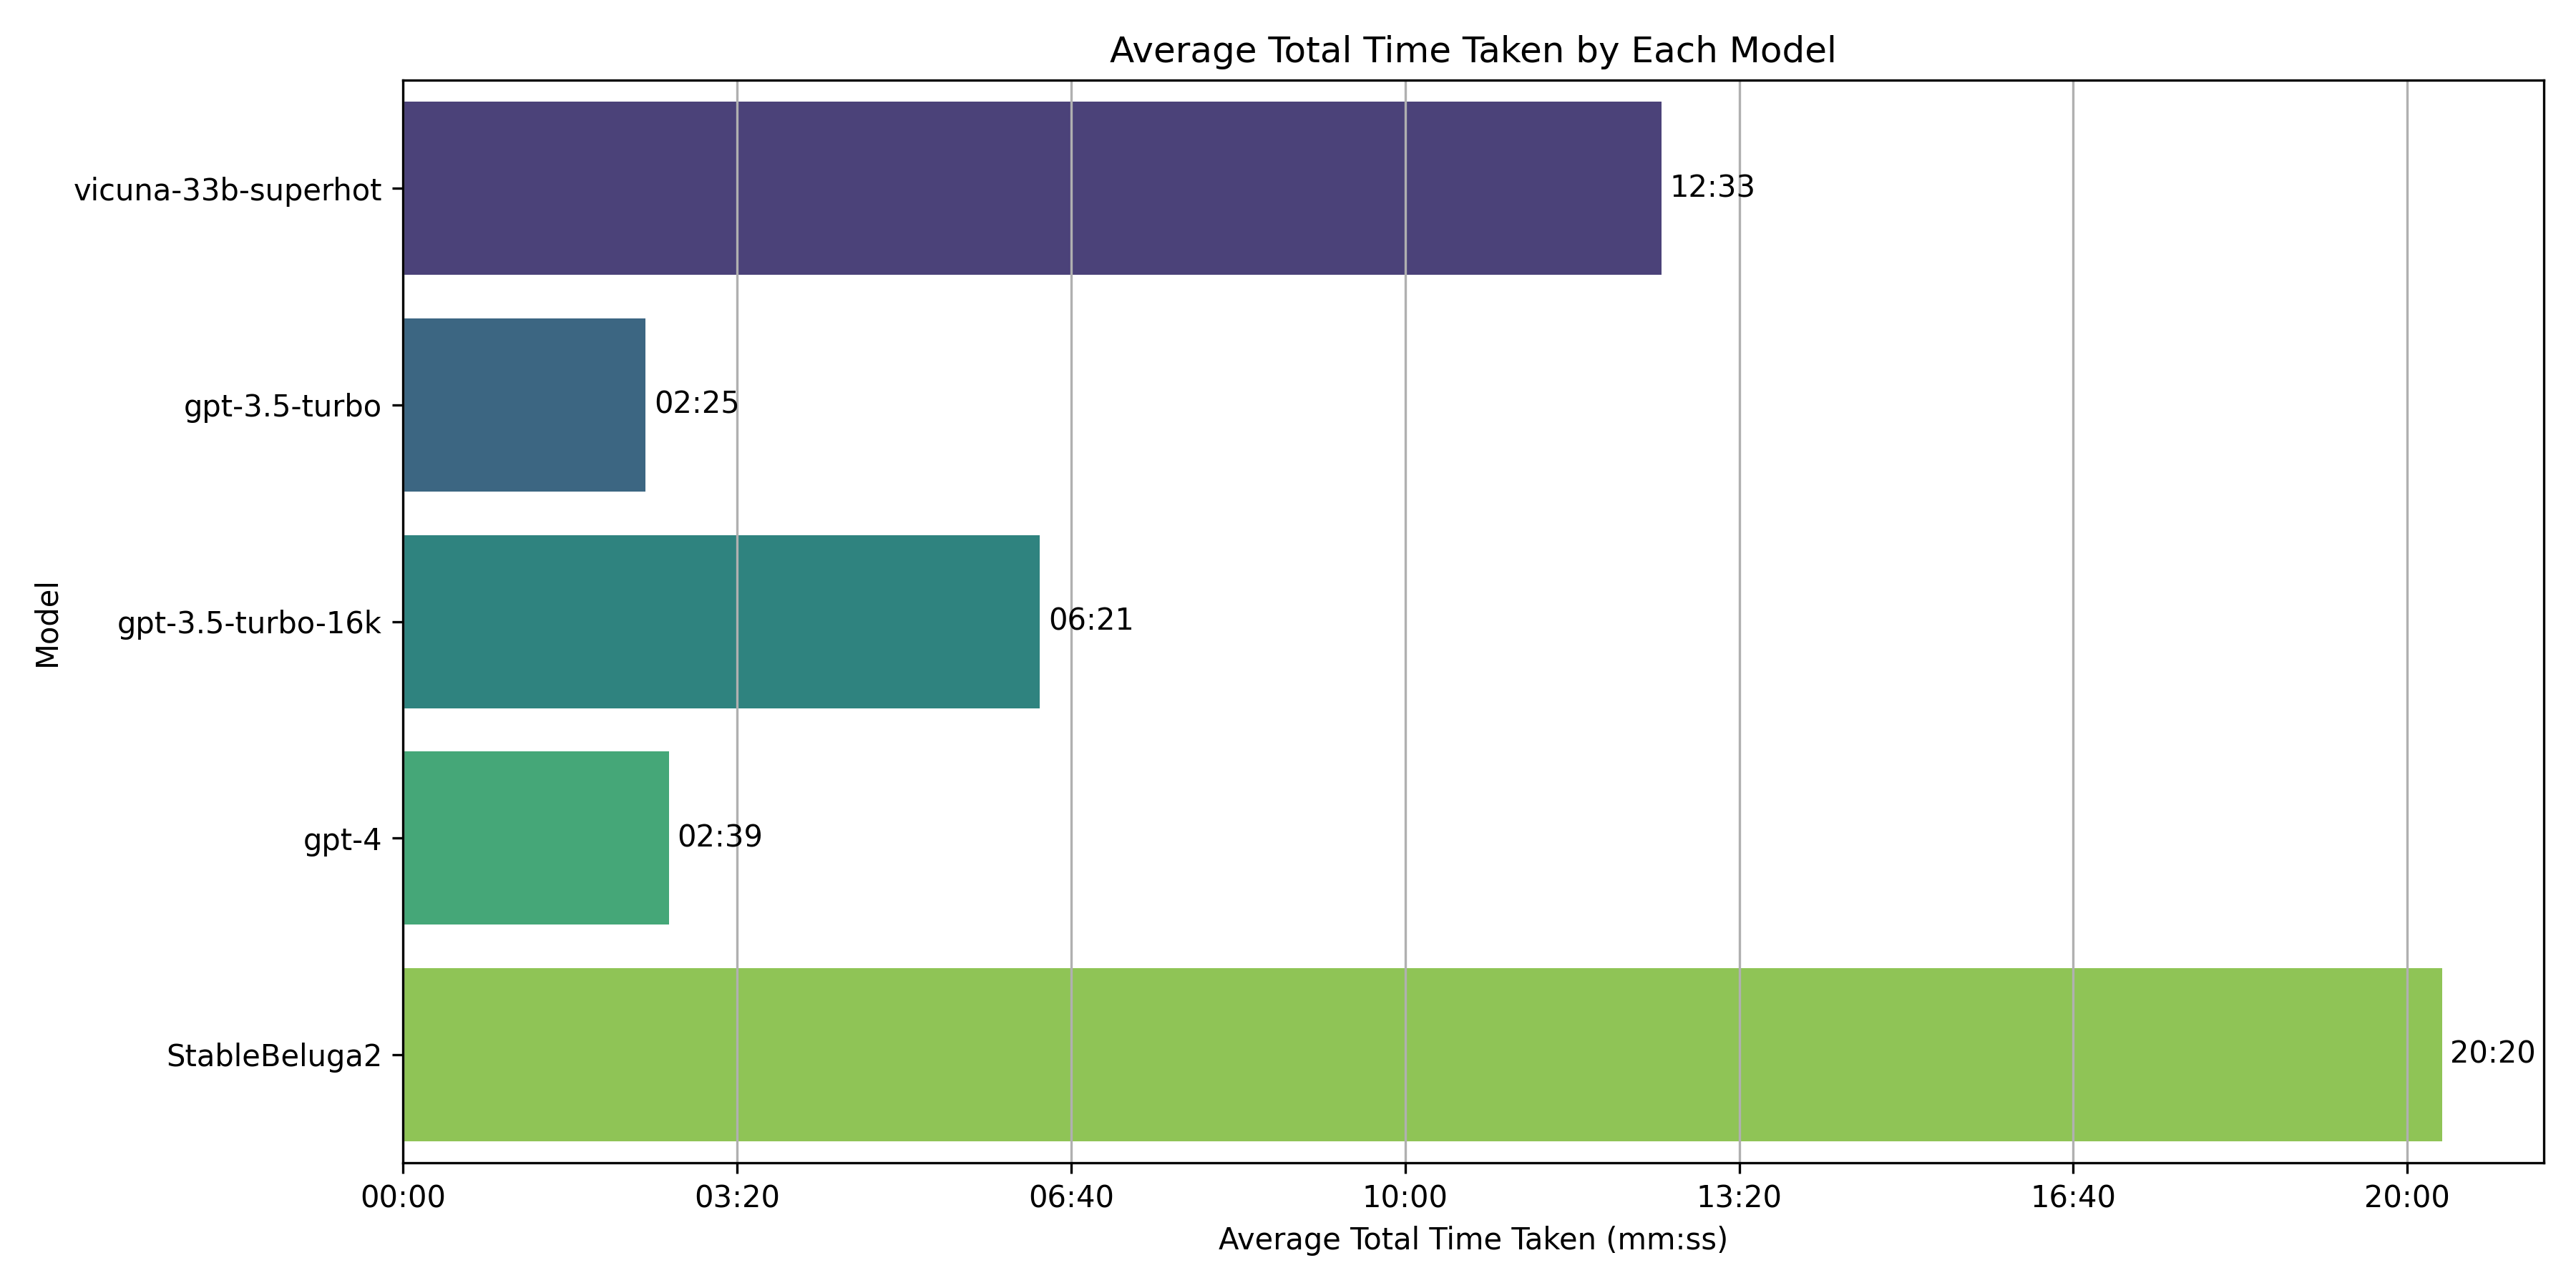
\includegraphics[width=14cm]{images/open-runtime.png}
  \end{tabular}
  \caption[Open Source Time]{Average Time Taken by all five models}\label{fig:open-runtime}
\end{figure}

\begin{figure}[htpb]
  \centering
  \begin{tabular}{c}
  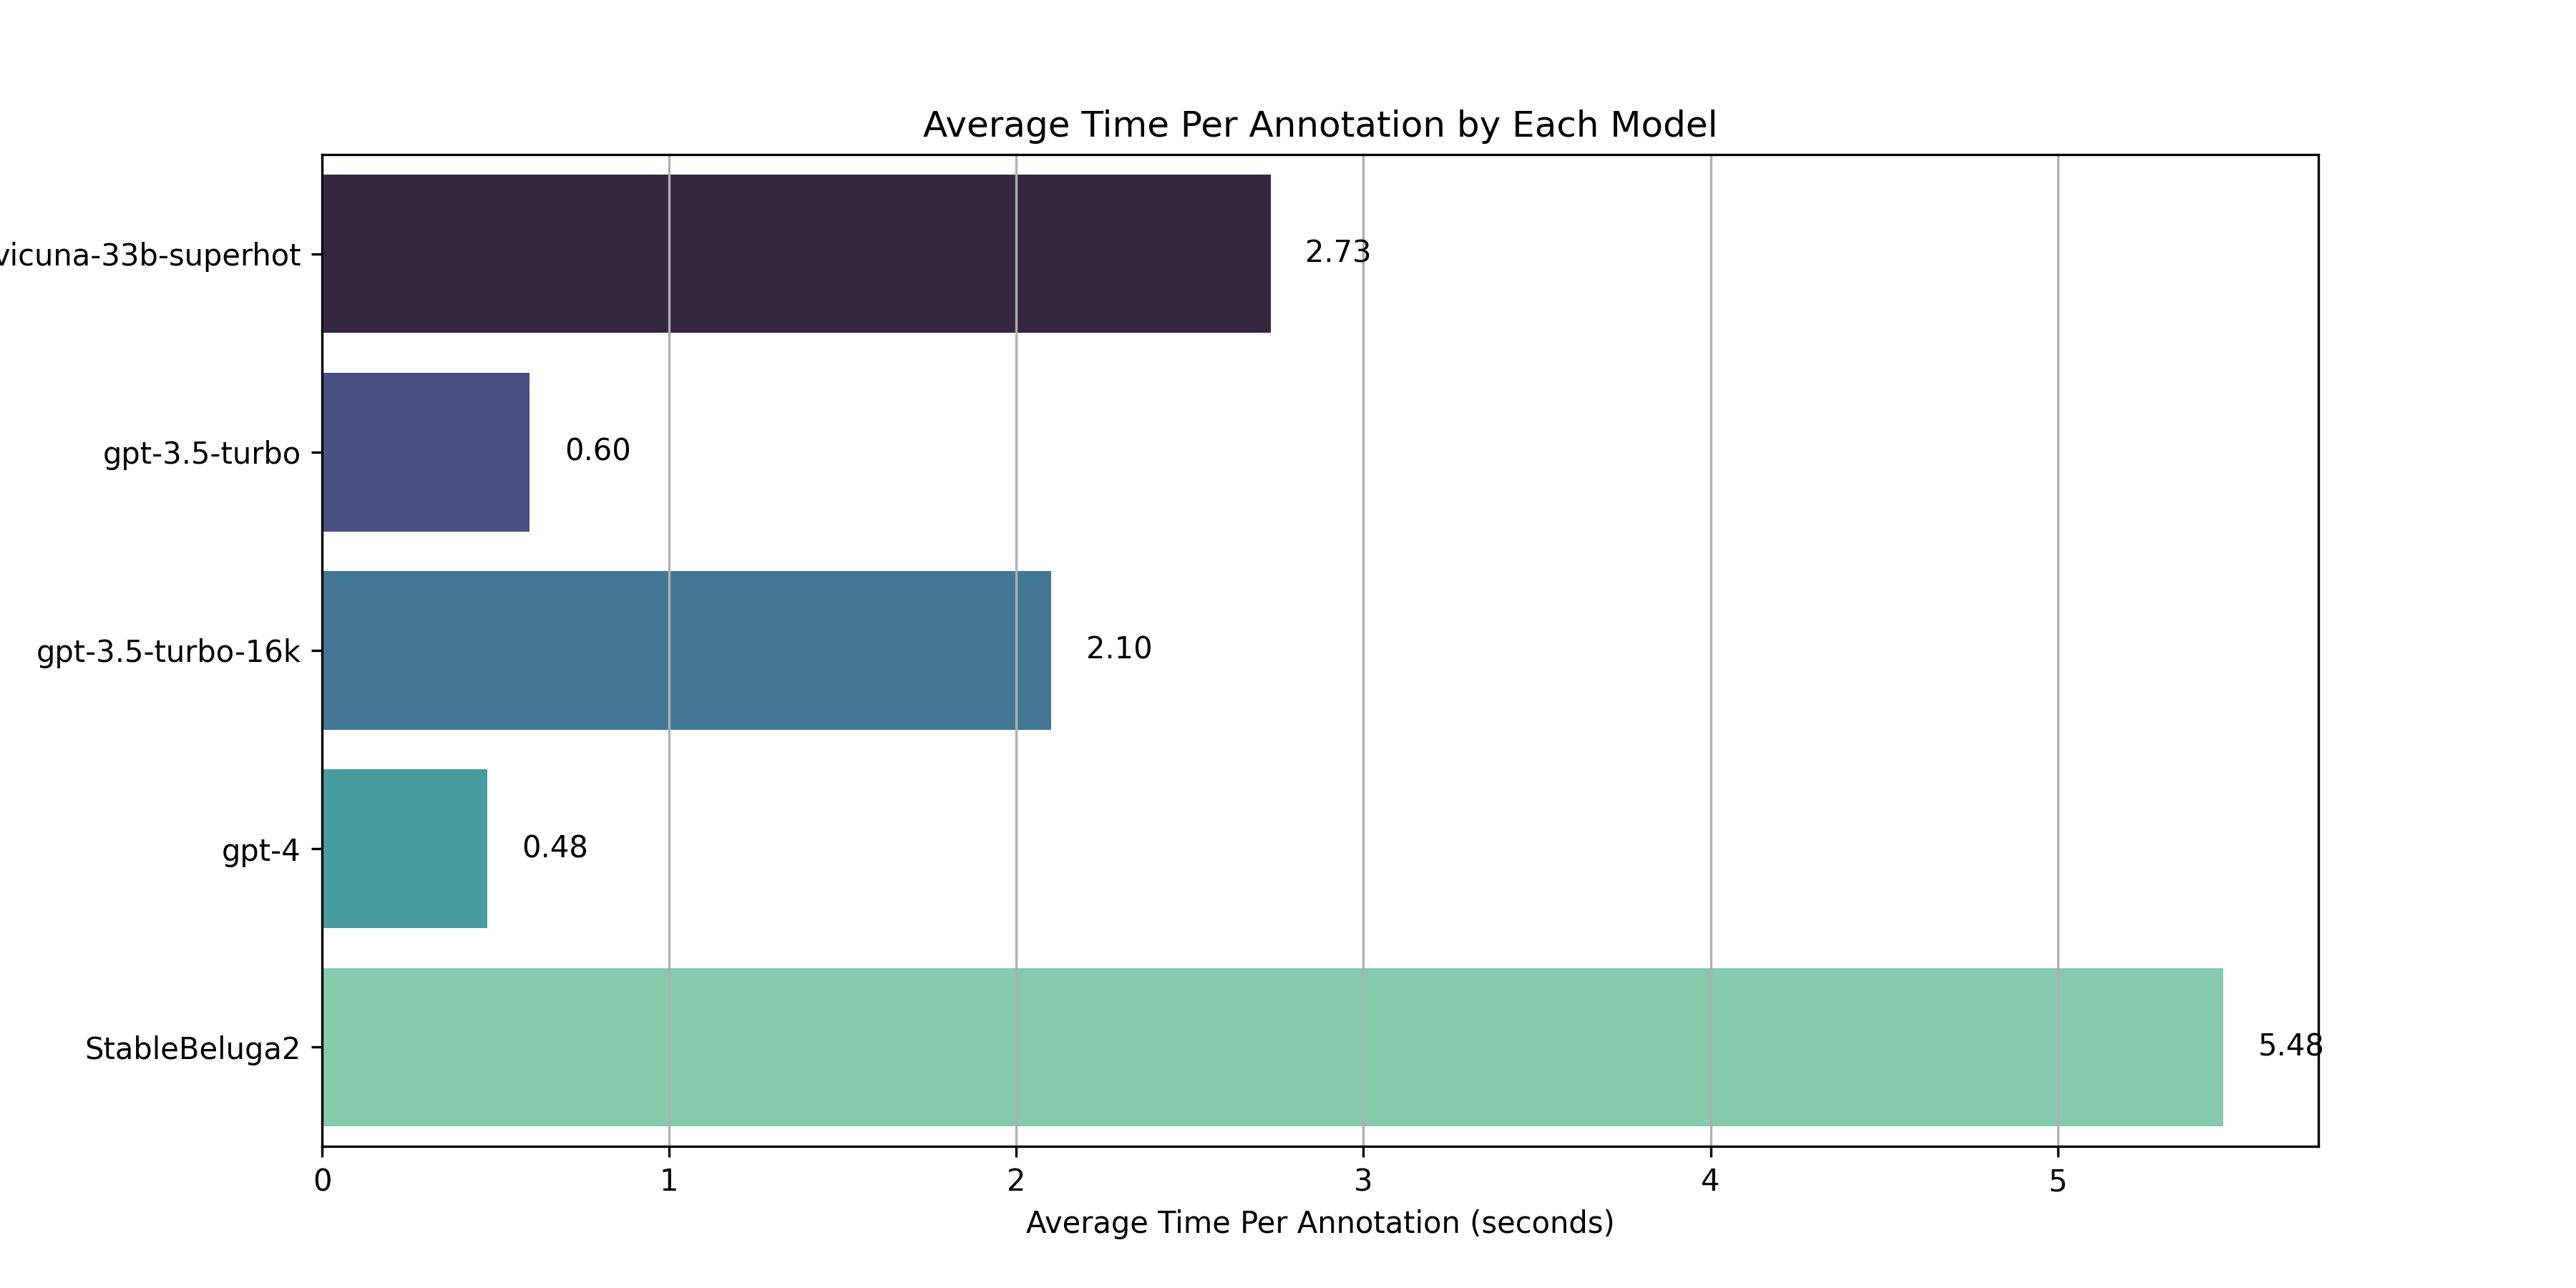
\includegraphics[width=14cm]{images/open-anno-cost.png}
  \end{tabular}
  \caption[Open Source Cost]{Average Time Taken Per Annotation by all five models}\label{fig:open-relative-cost}
\end{figure}

\begin{figure}[htpb]
  \centering
  \begin{tabular}{c}
  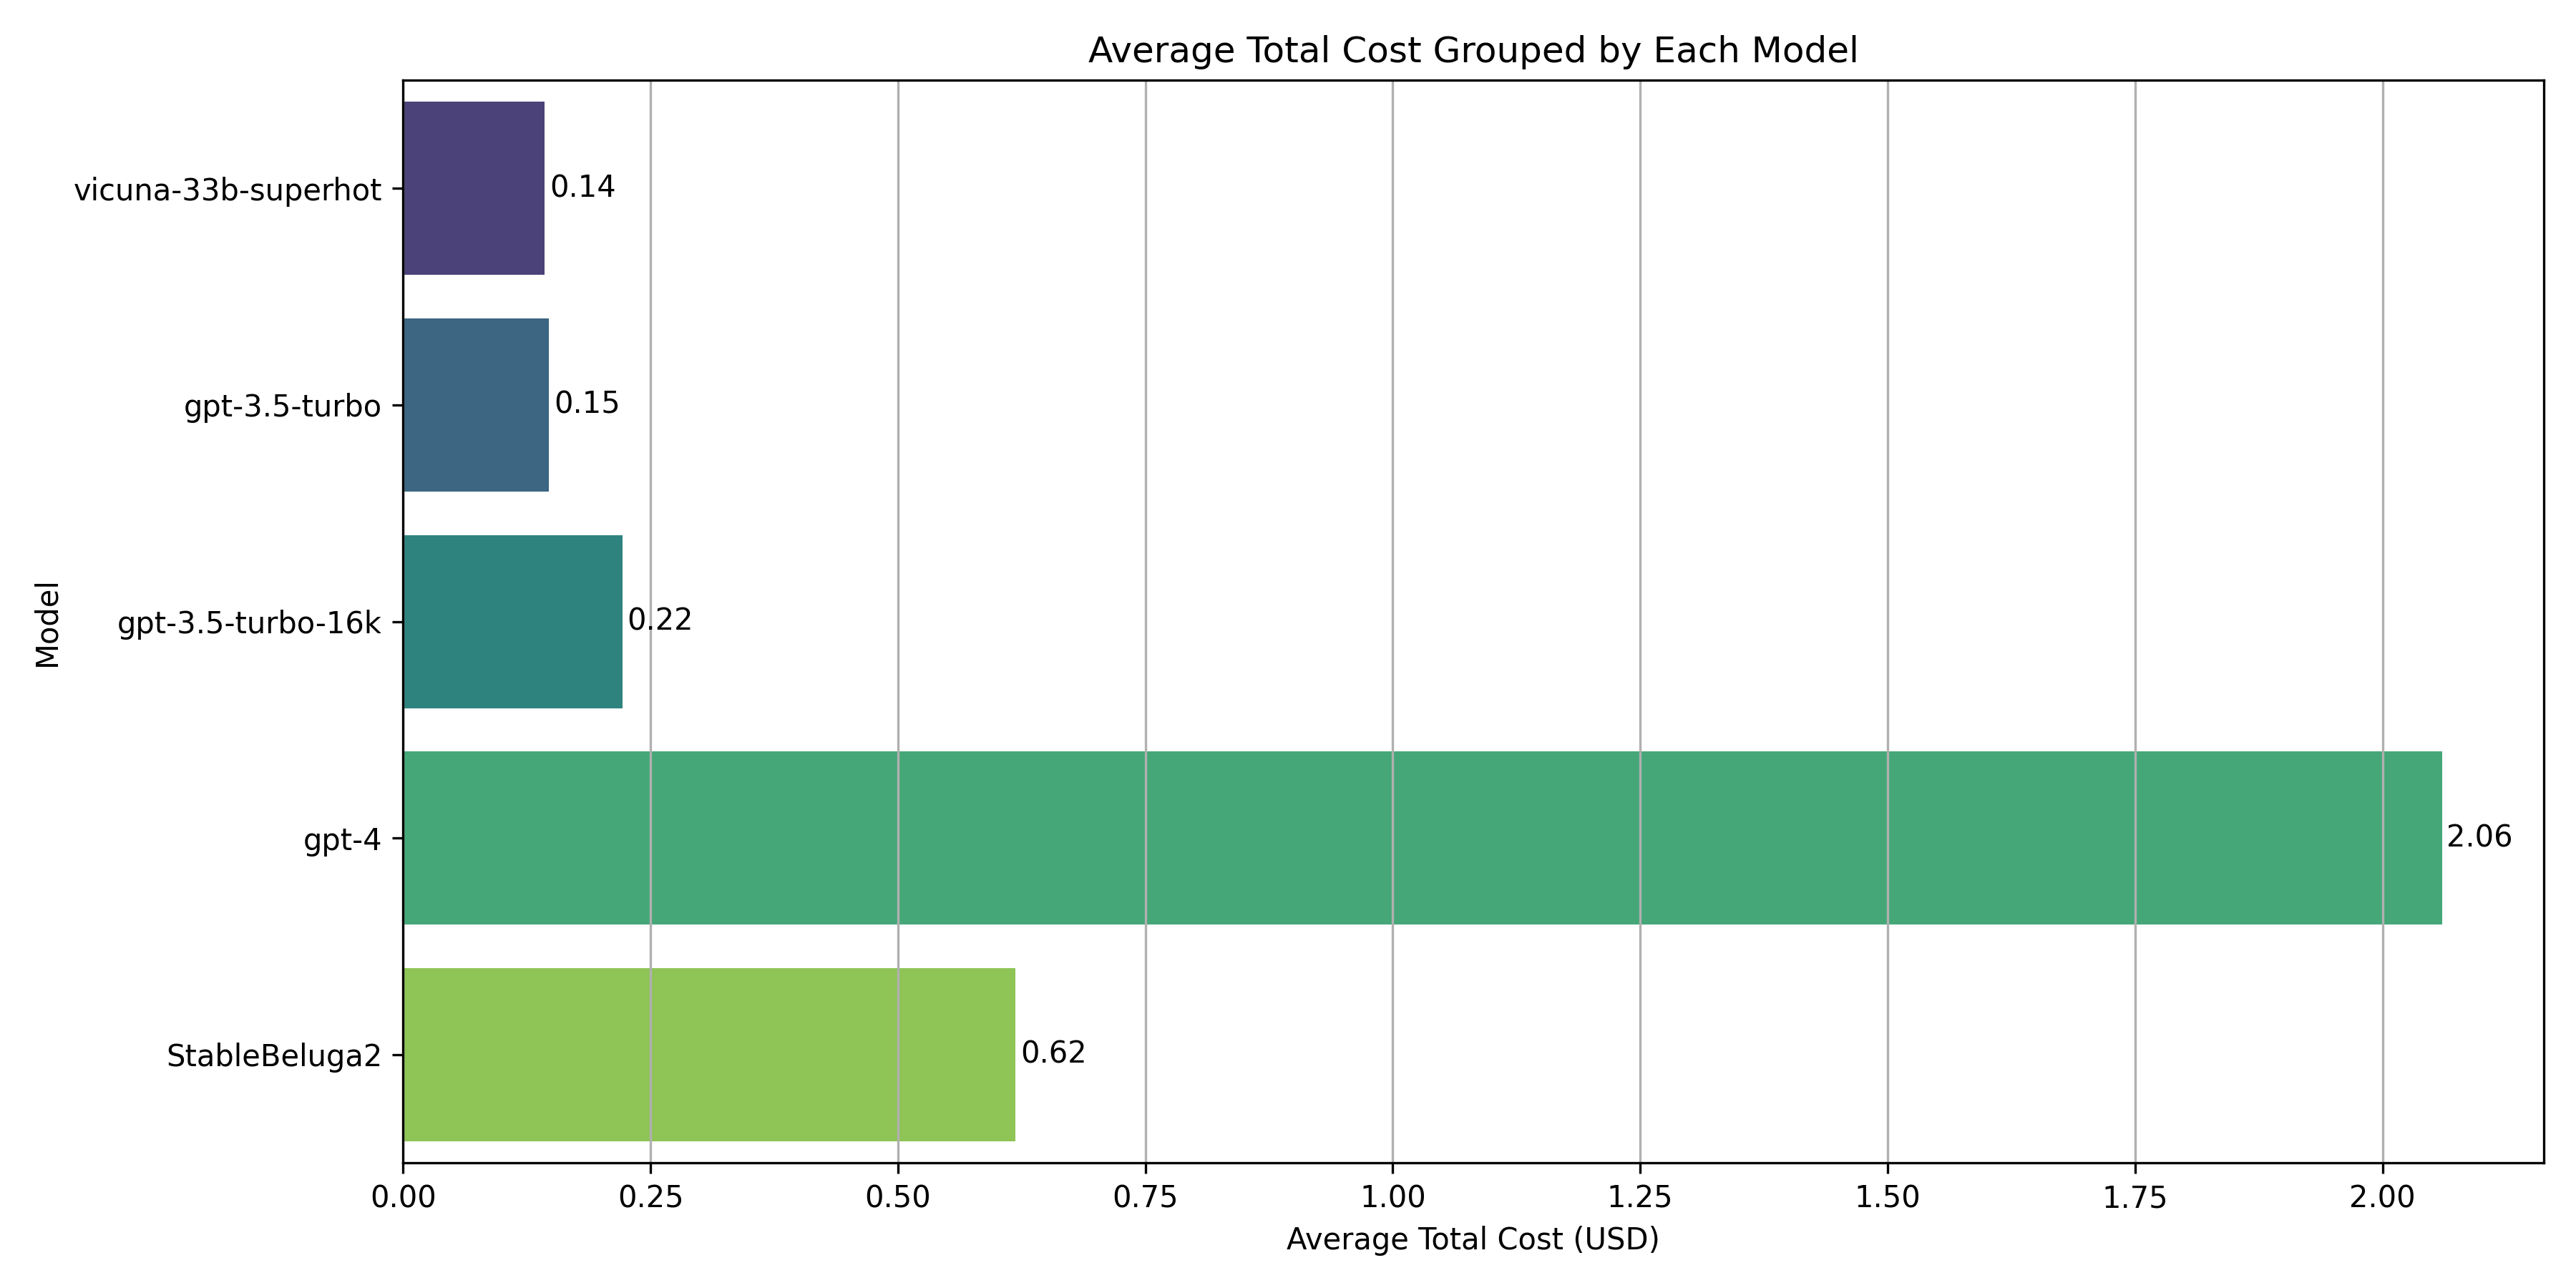
\includegraphics[width=14cm]{images/open-cost.png}
  \end{tabular}
  \caption[Open Source Time]{Average Paid Cost by all five models}\label{fig:open-cost}
\end{figure}

\section{Evaluating Potential Correlations}

Upon completion of our results assessment, it was fundamental to investigate potential correlations inherent in the received data. We probed two areas of interest: a potential correlation between the CoNLL Score and Semantic Accuracy and a possible linkage between the CoNLL Score and the paper's publication date. These examinations were crucial to determine whether any part of the original paper was contained within OpenAI's training data.

\subsection{Connection Between CoNLL Score and Semantic Accuracy}

Given that these two metrics reflect distinct facets of the paper, we anticipated that little to no correlation would be discernible. Nevertheless, several statistical measures were employed to thoroughly evaluate this potential relationship: Pearson's Correlation Coefficient, Spearman's Rank Correlation, and Kendall's Tau. As seen in Table \ref{tab:spearman}, the correlation results indicate a trivial association between these metrics, as the correlation constant is virtually zero, supported further by a notable high p-value.

\begin{table}[htpb]
    \centering
    \caption{Correlation Coefficients and P-values}\label{tab:spearman}
        \begin{tabular}{lrr}
        \hline
        Method & Correlation & P-value \\
        \hline
        Pearson's Correlation Coefficient & -0.1570 & 0.5472 \\
        Spearman's Rank Correlation & -0.0006 & 0.9981 \\
        Kendall's Tau & -0.0075 & 0.9670 \\
        \hline
    \end{tabular}
\end{table}

\subsection{Influence of Publish Date on CoNLL Score}

A query was raised regarding the possibility of papers released before September 2021—presumed to be the cut-off date for building OpenAI's GPT Models training data—yielding higher CoNLL Scores than those published afterwards. The difference in average CoNLL scores between papers released before was higher by 1.63 compared to those released after the deadline. This might be attributable to the variable nature of LLMs rather than the inclusion in the training set. For post-deadline papers, the semantic accuracy was also marginally lower—by an average of 5.87\%. However, this difference did not significantly suggest being due to training data influence.
Furthermore, the use of GPT to generate novel annotations makes it improbably likely for these exact or similar outputs to exist in the training dataset and affect the results. An observation worthy of mention is that the post-2021 papers contained significantly more concepts, which may have influenced the score. Henceforth, it is reasonable to conclude that a paper being part of the training dataset or not does substantially impact the score.

\section{Overall}

In comprehensive terms, GPT-4 established itself as the most effective and priciest model, while GPT-3.5 emerged as the cheapest and fastest. All GPT models provided commendable annotations for automation purposes, with the Open Source LLM StableBeluga2 marking a significant breakthrough with its zero-cost operation and performance that is almost at par with the GPT models. 

In comprehensive terms, GPT-4 emerged as the most impressive model due to its superior performance, albeit at a higher cost. GPT-3.5 was the most cost-effective and fastest model to operate. All GPT models provided commendable annotations for automation purposes, with the Open Source LLM StableBeluga2 marking a significant breakthrough with its zero-cost operation and performance that is almost at par with the GPT models. This is particularly noteworthy, considering StableBeluga2 is a 70 billion parameter model, and GPT-4 is rumoured to be a 1.8 trillion parameter model. The instructive nature of StableBeluga2, as opposed to the general-purpose chat model design of GPT, likely contributed to its performance in formula grounding. Figure \ref{fig:total-anal} visualises the performance-to-cost ratio for all five models, which helps to choose the models for different purposes.

\begin{figure}[htpb]
  \centering
  \subfloat[Average Cost per 1000 Concept]{
    \begin{tabular}{c}
  %\hspace*{-.25cm}
  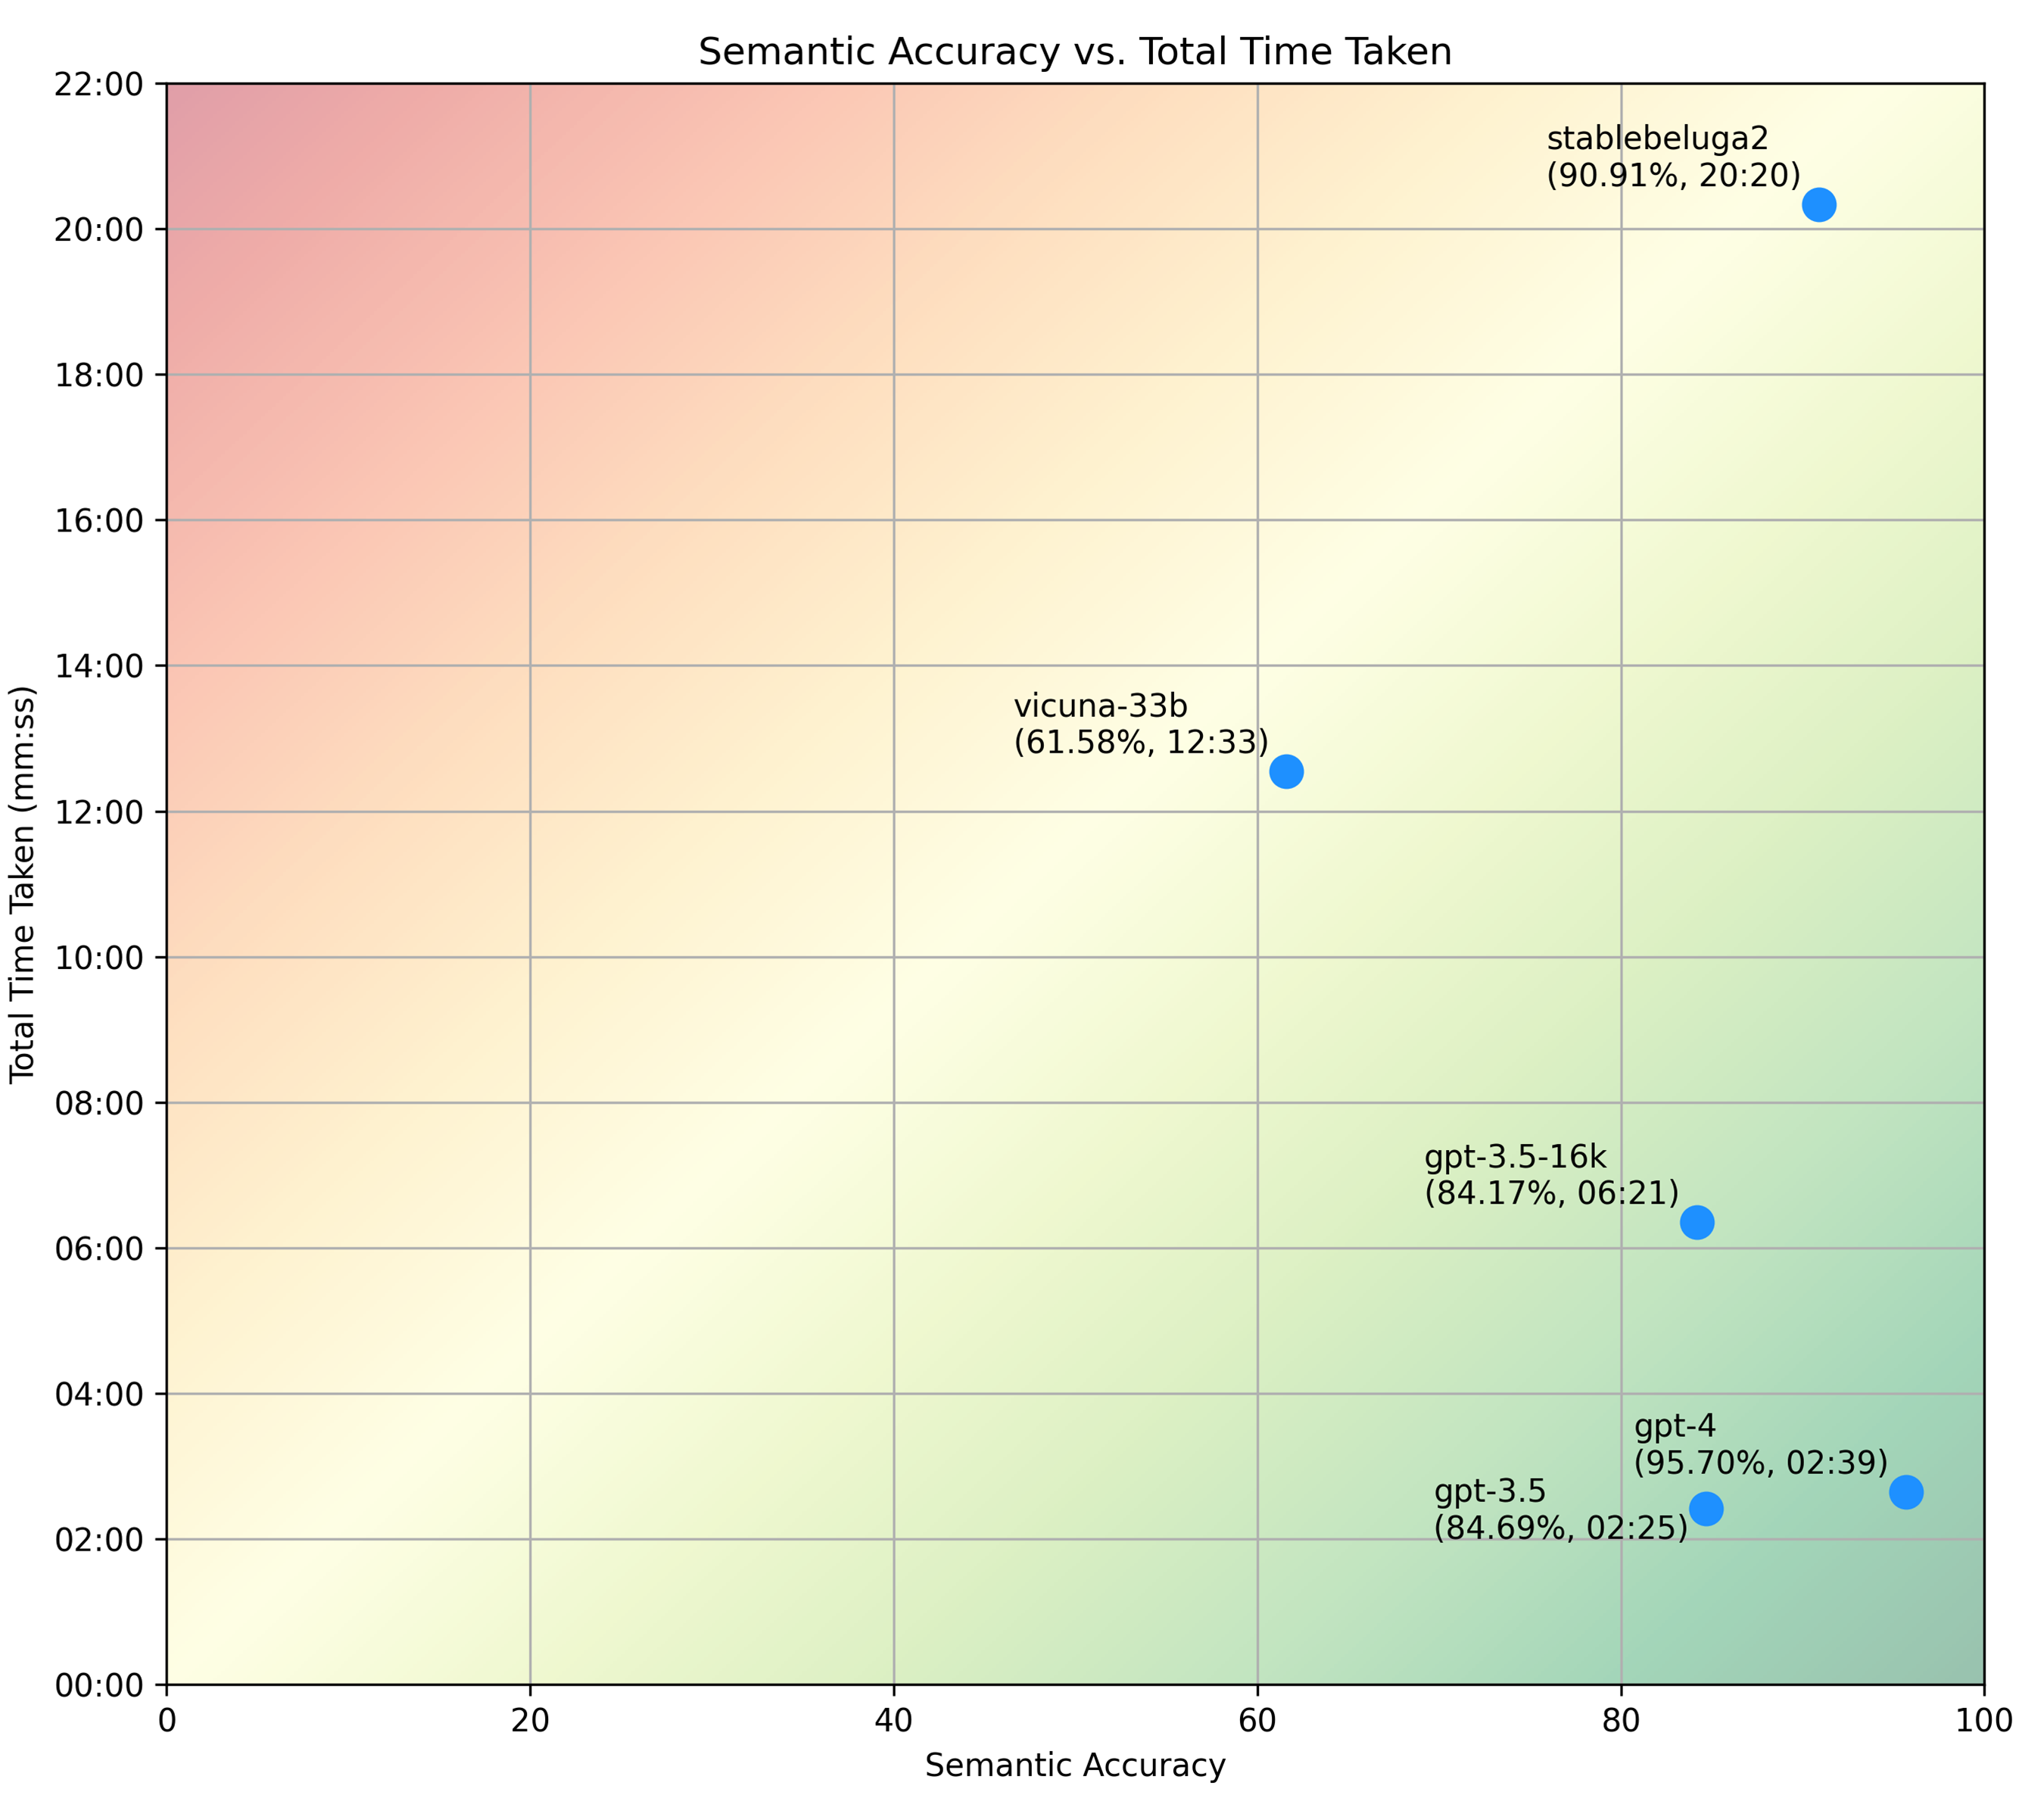
\includegraphics[width=10cm]{images/semantic-time.png}
  \end{tabular}
  }
  \quad 
  \subfloat[Average Duration per Concept]{
    \begin{tabular}{c}
  %\hspace*{-1.5cm}
  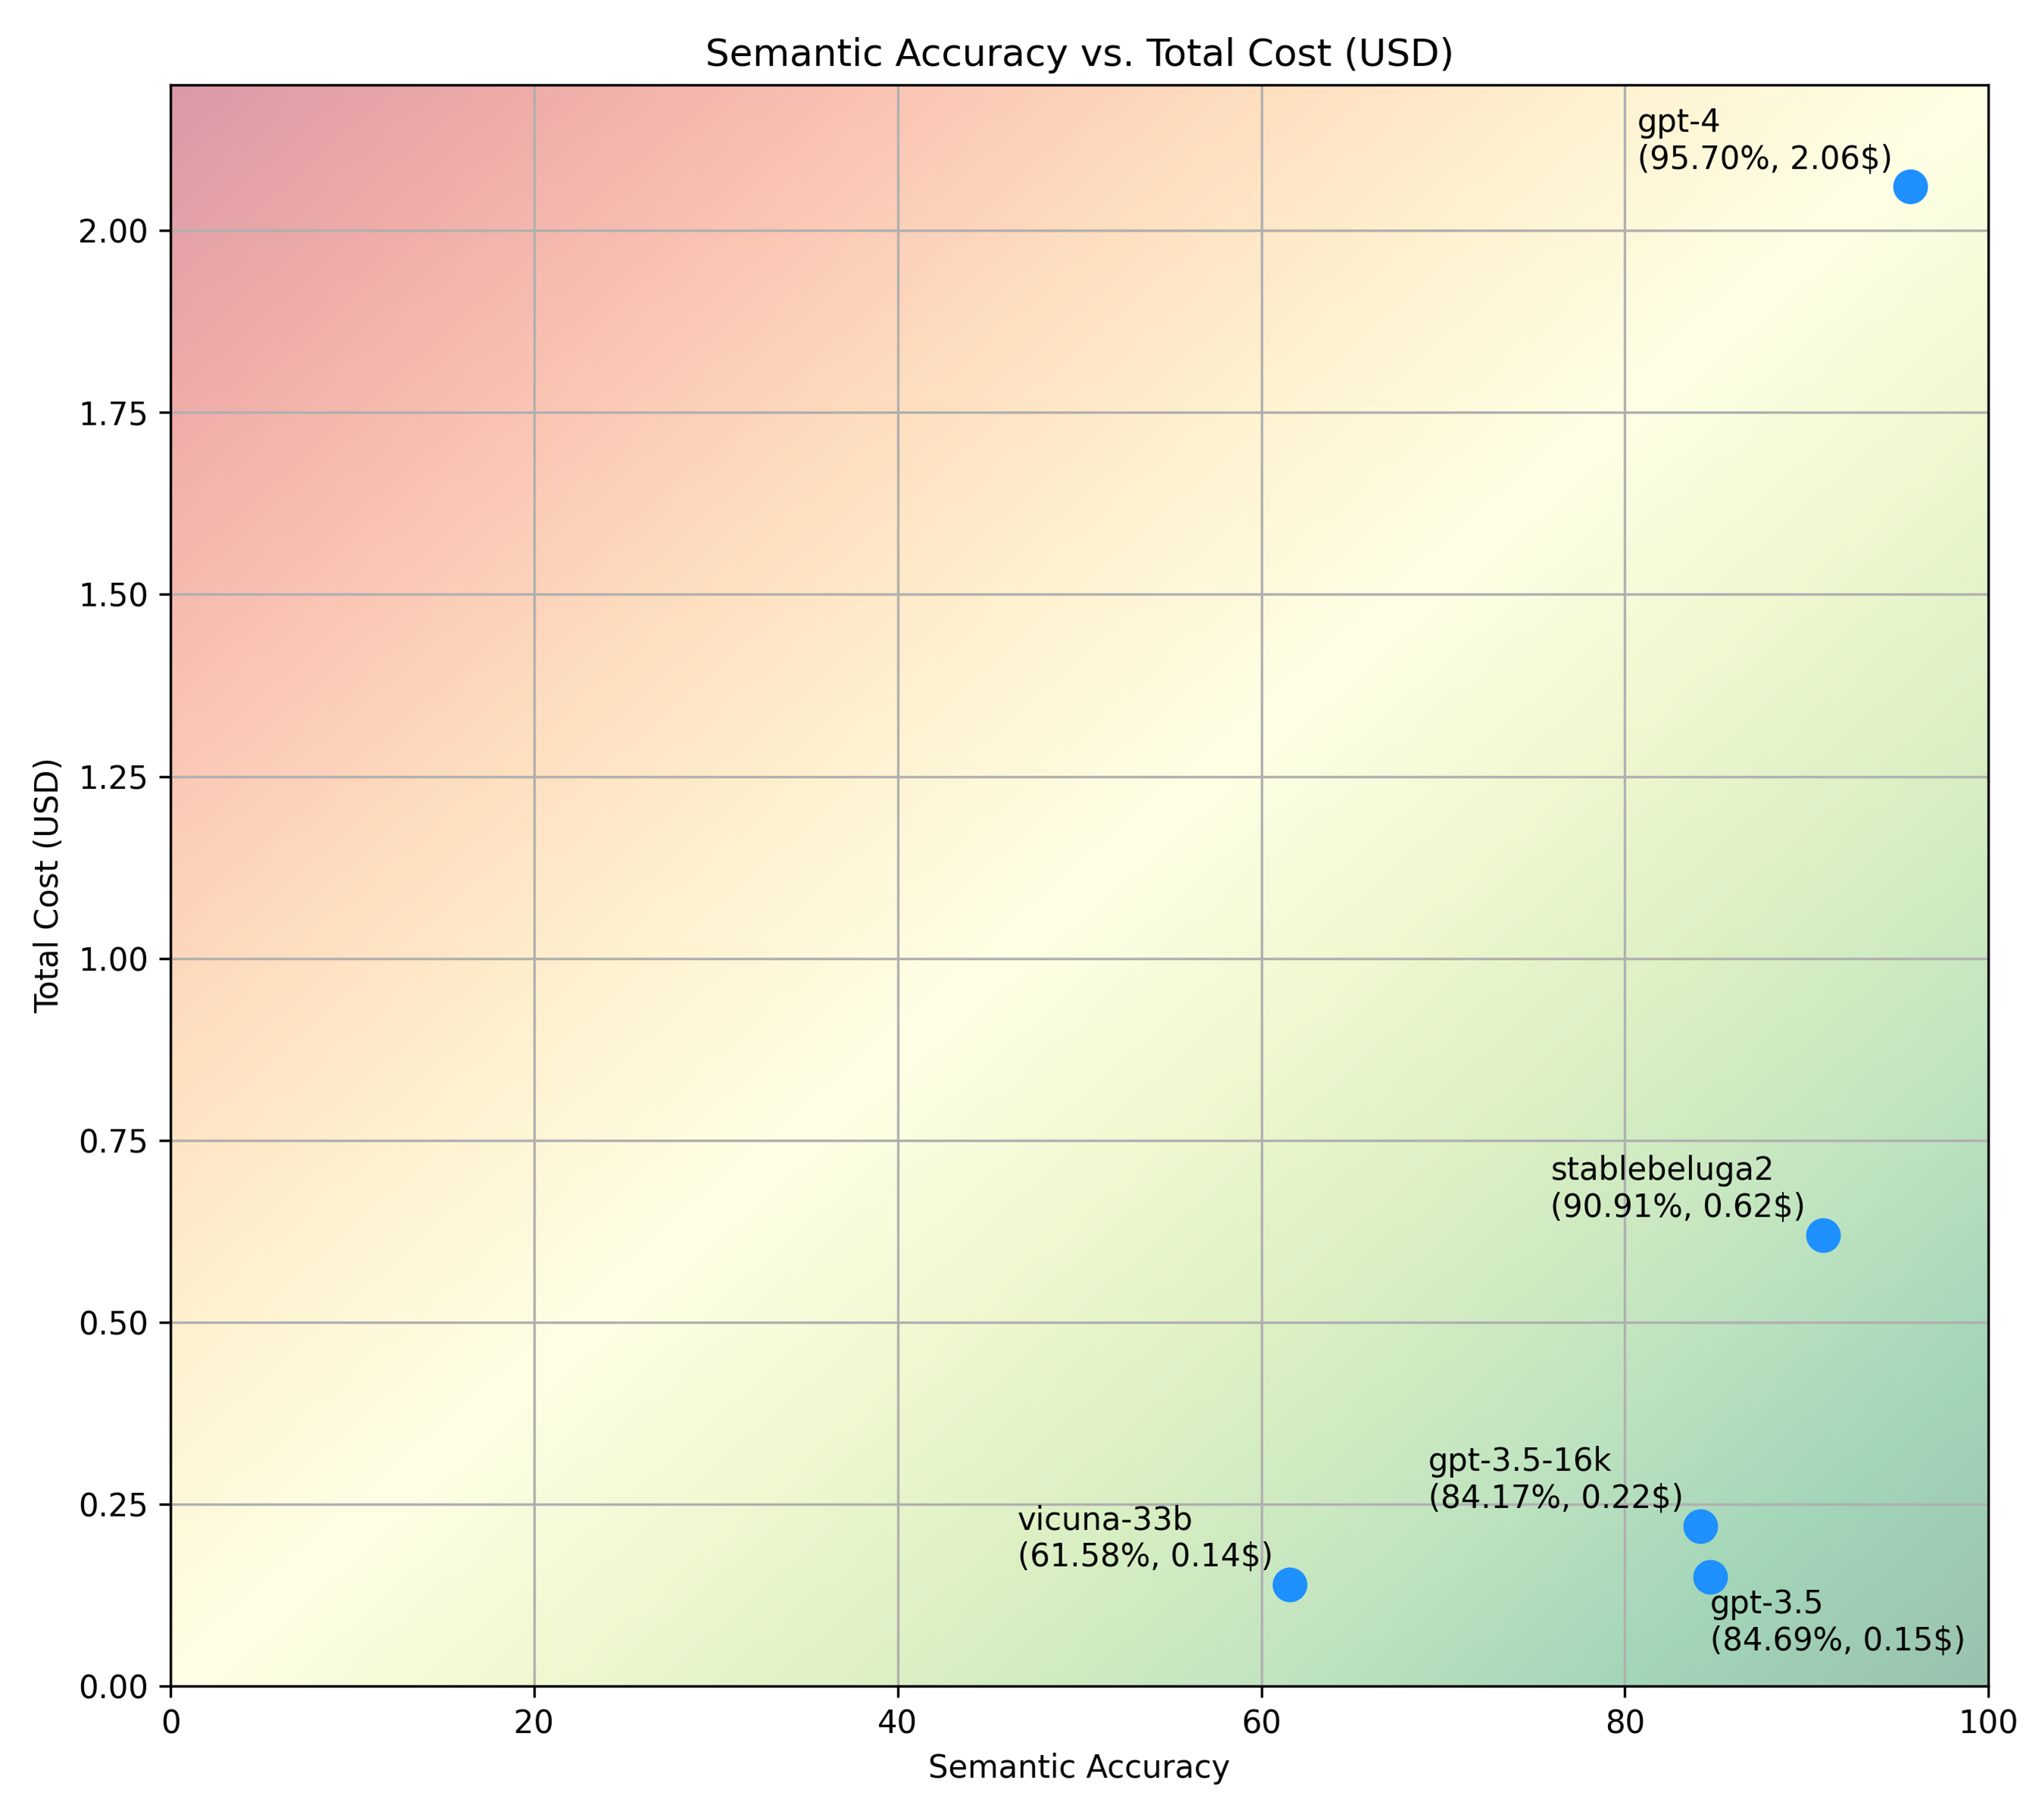
\includegraphics[width=10cm]{images/semantic-cost.png}
  \end{tabular}
  }
  \caption[Cost Analysis]{Cost and Time Usage of Automation}\label{fig:total-anal}
\end{figure}

\chapter{Future Works}\label{chapter:future_works}
\chapter{Conclusion}\label{chapter:conclusion}
% TODO: add more chapters here

\appendix{}

\microtypesetup{protrusion=false}

\addchap{Abbreviations}
\begin{acronym}
	\itemsep-.25\baselineskip
	\acro{TUM}[TUM]{Technical University of Munich}
	\acro{LLMs}[LLMs]{Large Language Models}
	\acro{NLP}[NLP]{Natural Language Processing}
	\acro{POS}[POS]{Part-of-Speech}
	\acro{CoNLL}[CoNLL]{Computational Natural Language Learning}
	\acro{MioGatto}[MioGatto]{Math Identifier-oriented Grounding Annotation Tool}
\end{acronym}

\listoffigures{}
\listoftables{}
\microtypesetup{protrusion=true}
\printbibliography{}

\end{document}
